\part{休  克}

\chapter{休 克 概 论}

休克(shock)是指机体由于受到外来的或内在的强烈致病因素打击或两者共同作用而出现的以机体代谢异常和循环功能紊乱为主的一组临床综合征,这些致病因素包括大出血、创伤、中毒、烧伤、窒息、感染、过敏及心脏泵功能衰竭等。1743年法国医生Henri
Francois Le
Dran首次报告了严重外伤后的“choc”现象,认为休克是由于中枢神经功能紊乱导致的循环以及其他器官功能不全的危重状态。此后,Warren在19世纪后期又将创伤性休克描述为面色苍白或发绀、四肢湿冷、脉搏细速、尿少和神经淡漠的“濒死状态”,Crile后来又补充了“低血压”这一重要特征,这些特征性描述已经基本上反映出了休克的主要临床特点。20世纪60年代后,随着Lillehei提出的“微循环障碍学说”的创立以及基础研究的深入发展,对休克现象的认识水平逐步提高。目前认为休克是各种病因所致的急性血液循环障碍,是一个以低血压和微循环灌注锐减为特点、导致重要器官灌注不足、组织氧供(O\textsubscript{2}
supply)和氧需(O\textsubscript{2}
demand)失衡以及细胞功能紊乱和代谢障碍的危重病理过程。

\subsection{病因与发病机制}

休克的发生的病理生理过程与其诱因密切相关,其分类也以病因学分类为主,目前对于休克分类尚无统一认识,临床上可根据休克发生的始动特点将其简明地分为三大类:①低血容量性(hypovolemic)休克,包括失血性(hemorrhagic)、烧伤性(burn)和创伤性(traumatic)休克三种,其共同环节都有血容量的降低;②血管扩张性(vasodilatory)或者分布性(distributive)休克,包括感染性或者脓毒症(septic)、过敏性(anaphylactic)和神经源性(neurogenic)休克三种;③心源性(cardiogenic)休克,包括心脏本身病变、心脏压迫或梗阻引起的休克。美国外科医师学会把由于心脏外因素包括大面积肺栓塞、心包填塞及缩窄性心包炎等所致的心脏泵功能障碍单独归类为梗阻性(obstructive)休克,但其血流动力学特点与心脏本身疾患所致休克的特点类似。

另外,按休克时血液的动力学的特点也可分为两类,即低排高阻型休克或称低动力型休克(hypodynamic
shock)和高排低阻型休克或称高动力型休克(hyperdynamic
shock)。低动力型休克临床上常见,包括了低血容量性、心源性和大多数感染性休克,特点是心脏排血量低,而总外周血管阻力高,由于皮肤血管收缩,血流量减少,使皮肤温度降低,故又称为“冷性休克(cold
shock)”;而高动力型休克常见于部分感染性休克,其总外周血管阻力低,心脏排血量高,由于皮肤血管扩张,血流量增多,使皮肤温度升高,故亦称“温性休克(warm
shock)”。

\subsubsection{病因}

\paragraph{低血容量性休克}

患者发生低血容量性休克的内在原因在于血管内容量(绝对或相对)不足,并由此引起心室充盈不足和心搏量减少,如果增加心率仍不能代偿,可导致心排量降低。血流动力学特点表现为心室前负荷下降并导致心室舒张末压力及容积、每搏量、心输出量降低,最终导致血压下降。休克严重程度与液体损失程度及速度密切相关。一般15分钟内失血少于全身循环血量的10\%时,机体可通过加快心率及增加体循环阻力(SVR)进行代偿,使血压和组织灌流量保持稳定。若快速失血量超过循环血量的20\%左右,机体将开始处于失代偿状态,SVR显著上升,组织微循环血流下降,无氧酵解增强,乳酸水平开始上升。当失血量超过循环血量40\%时,患者表现出明显的休克体征。

低血容量性休克的常见的原因为急性出血,但亦可由于体液丧失增加造成。后者发展到低血容量常需数小时以上,过程相对较隐匿,由于血液浓缩,可伴血红蛋白(Hb)或血细胞比容(Hct)增加。①失血性休克:是指因大量失血,迅速导致有效循环血量锐减而引起外周循环衰竭的一种综合征。常见于消化性溃疡、食管静脉曲张、主动脉夹层破裂以及妊娠或生产等原因引起的大出血,出血可为显性(如呕血或黑粪)或隐性(如异位妊娠破裂)。②烧伤性休克:大面积烧伤,伴有血浆大量丢失,可引起烧伤性休克。休克早期与疼痛及低血容量有关,晚期可继发感染,发展为感染性休克。③创伤性休克:严重创伤可导致创伤性休克,这种休克的发生与疼痛刺激和失血有关。

\paragraph{血管扩张性休克}

这类休克通常是由于血管扩张所致的血管内容量相对不足,其循环血容量正常或增加,但心脏充盈和组织灌注不足,很多情况下存在着广泛的静脉或小动脉扩张。血管阻力减低而心排量不能相应增加使得体循环血压下降、器官灌注不良,当冠脉灌注不足时可继发出现心肌功能不全或其他病理机制(如心肌抑制因子或其他毒性物质的释放),使血管扩张所致的休克复杂化。其最主要特点是外周血管扩张,毛细血管通透性增加,液体渗漏,有效循环血量下降,前负荷降低。常见于以下三种:①感染性休克:是临床上最常见的休克类型之一,各种病原微生物感染严重时均可引起感染性休克,临床上以G\textsuperscript{−}
杆菌感染最常见。细菌内毒素作用是导致感染性休克微循环障碍和炎性器官功能损害的重要因素。根据血流动力学的特点又可将其分为低动力型的冷休克和高动力型的暖休克两型。②过敏性休克:由IgE介导的Ⅰ型超敏反应引起。已致敏的机体再次接触到抗原物质时,可发生强烈的变态反应。IgE激活肥大细胞或嗜碱性粒细胞,导致组胺、白介素、缓激肽、前列腺素等炎症因子大量释放入血,使患者全身容量血管扩张,毛细血管通透性增加和支气管痉挛,继之出现的弥散性非纤维蛋白血栓、血压下降、组织灌注不良可使多脏器受累。最近的文献提示,人群中有1\%~2\%的人可能发生过敏性休克。这类休克常见的变应原有药物(如青霉素、神经肌肉阻断剂)、花粉、海鲜或其他特殊蛋白制品、某些蚊虫叮咬所传播的寄生虫等。治疗上主要是通过去除变应原,补液、注射肾上腺素改善血流动力学状态。③神经源性休克:交感神经系统急性损伤或被药物阻滞可引起受累神经所支配小动脉扩张,血容量增加,出现相对血容量不足和血压下降。这类休克预后好,常可自愈。常见原因有剧痛、脊髓麻醉或损伤等。

\paragraph{心源性休克}

心源性休克常是指患者心脏泵功能受损或心脏血流排出道受阻,心输出量下降,代偿性血管收缩不足,导致有效循环血量不足、低灌注和低血压。心脏因素包括大面积急性心肌梗死、心肌病变、心脏手术、缺血再灌注损伤和严重的心律失常等,以及心外阻力因素心包填塞、张力性气胸等,常是引起心源性休克的原因。

美国外科医师学会把此类以心脏泵功能衰竭为主要特点的休克分为狭义的(心脏性)心源性休克和梗阻性休克,分别指由于心脏本身原因包括心肌或者瓣膜结构异常所致的休克和由于心脏外因素包括大面积肺栓塞、心包填塞及缩窄性心包炎所致的休克。心脏本身原因引起休克是由于心脏本身泵动力不足所致,表现为持续的低血压(收缩压<
90mmHg,或比基础血压下降超过30mmHg)、心脏指数严重下降{[}未治疗情况下<
1.8L/(min•m\textsuperscript{2}
){]}及心室充盈压力增高(左室舒张末压力> 18mmHg或右室舒张末压>
10~15mmHg),外周血管、神经内分泌系统及炎症因子在此类休克的发生及发展过程中起一定作用。而梗阻性休克出现于心包填塞造成的心脏舒张受限或者大面积肺栓塞的情况下,此时患者血液回流受阻,右室后负荷增加,心输出量下降,但心脏本身的收缩和舒张功能正常。梗阻性休克的临床表现与疾病的发病速度有关,心肌梗死后的心肌破裂可导致心包腔在数分钟内积聚150ml左右的血液,这足以压迫心脏而出现休克,需要立即引流和手术;肿瘤或炎症所致的心包腔内积液,液体积聚速度较慢,当液体体积到达1~2L时才可能出现休克。

不同类型休克血流动力学改变基本特点见表\ref{tab19-1}。为便于与美国外科协会的四类休克的分类法比较,以下把心脏外的外源性因素所致的梗阻性休克与心脏本身因素所致的休克分别列出。从其特点可见,两者休克的血流动力学改变的基本特点类似,这也是笔者把两者合并阐述的基本依据。

\subsubsection{发病机制}

机体承受的内在或外在打击足够剧烈时,均可导致休克现象。休克是一个有着复杂病理生理过程的临床综合征。虽然休克的病因各异,类型不一,临床表现也不尽相同,但其本质相同,即休克发生后机体重要器官微循环处于低灌流状态,导致细胞缺血缺氧,细胞代谢异常,继续发展可导致细胞损害、代谢紊乱,组织结构损伤,重要器官功能失常,最终可出现MODS。

在临床方面,及时发现并解除休克成因、纠正低血压状态有助于休克治疗,但这些并不意味着休克引起的内环境紊乱或并发症会随之改善,有时休克时出现的组织器官功能损害反而会继续发展并造成病情反复加重,此即所谓的重症难治性休克状态(irreversible
shock
state),这些特点提示我们在处理休克时要重视其发病机制,对其过程和特点有全面、深入的认识。

\hypertarget{text00055.htmlux5cux23CHP2-1-1-2-1}{}
(一) 休克时微循环变化及机制

1964年
Lillehei提出的休克微循环障碍学说目前已得到大多数学者的认可,许多新研究使微循环学说的内容更加丰富。虽然,休克成因不同,休克不同阶段组织灌流量减少的机制各异,但体内重要器官微循环处于低灌流状态的特点是相近的,下面以典型的失血性休克为例从时相变化和血流变化两方面分析其微循环障碍的特点。

\paragraph{时相变化}

\hypertarget{text00055.htmlux5cux23CHP2-1-1-2-1-1-1}{}
(1) 缺血性缺氧期(休克代偿期):

休克早期,微血管系统持续痉挛,口径明显缩小,毛细血管前阻力显著增加,血管自律运动增强,同时大量真毛细血管网关闭,毛细血管血流限于直捷通路,动静脉吻合支开放,组织灌流减少,出现少灌少流,灌少于流的情况。这一现象在皮肤、肌肉、肾脏等脏器尤为显著,其结果是保证了心、脑等重要器官的供血,对维持有效循环血量、回心血量及血压有一定代偿意义。机体出现微循环血管持续痉挛的始动因素是交感-肾上腺髓质系统兴奋。休克时大量儿茶酚胺释放入血,血中儿茶酚胺含量比正常高几十倍甚至几百倍。儿茶酚胺大量释放,既刺激α受体,造成皮肤、内脏血管明显痉挛,又刺激β受体,引起大量动静脉短路开放,构成了微循环非营养性血液通路,使器官微循环血液灌流锐减。此外,休克时体内产生的其他体液因子,如血管紧张素Ⅱ、加压素、内皮素、心肌抑制因子(MDF)、血栓素(TXA\textsubscript{2}
)和白三烯等物质等也都有收缩血管的作用。

\begin{table}[htbp]
\centering
\caption{不同类型休克血流动力学改变基本特点}
\label{tab19-1}
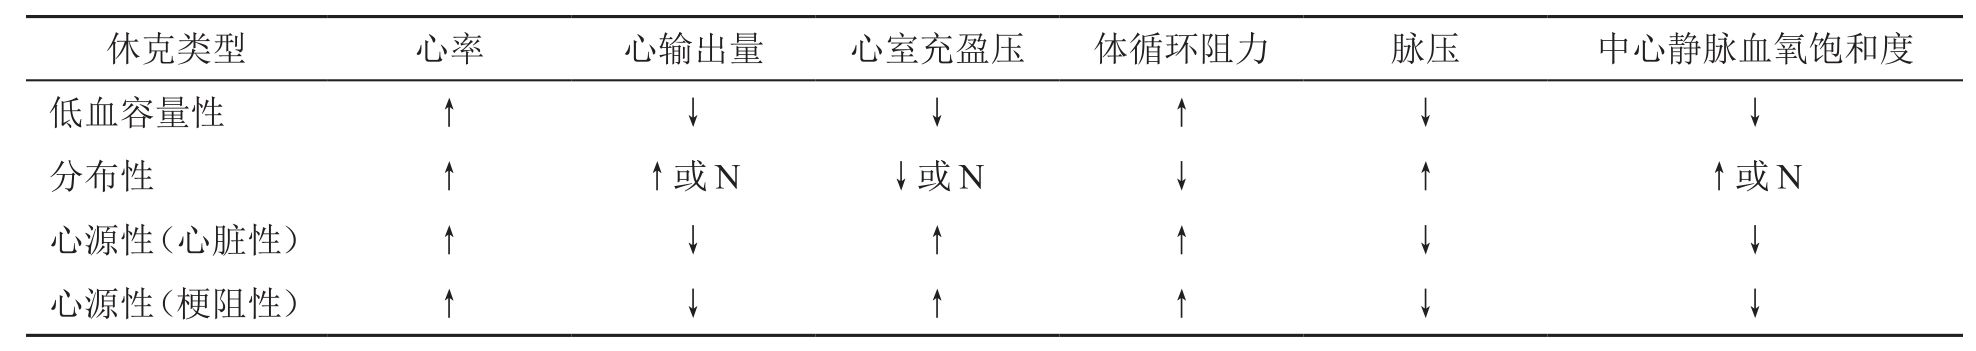
\includegraphics[width=6.58333in,height=1.16667in]{./images/Image00083.jpg}
\end{table}

N:正常

\hypertarget{text00055.htmlux5cux23CHP2-1-1-2-1-1-2}{}
(2) 淤血性缺氧期(可逆性失代偿期):

随着休克持续,微循环中血管自律运动首先消失。血管床对儿茶酚胺的反应进行性降低,微动脉和毛细血管前括约肌收缩逐渐减退,血液大量涌入真毛细血管网,而毛细血管的流出道的阻力增加,血液淤积在毛细血管中,微循环灌注量进一步下降。此时,内脏微循环出现灌流减少和血液淤滞现象,失代偿期的出现与长时间血管收缩、缺血缺氧及多种体液因子形成有关。首先,随休克病程发展,逐渐出现血管收缩因子和舒张因子间平衡失调,这种平衡失调的发生与休克时持续缺血缺氧使组织氧分压下降、CO\textsubscript{2}
和乳酸堆积、酸中毒有关:①酸中毒导致平滑肌对儿茶酚胺的反应性降低;②皮肤和腹腔内脏长期缺血缺氧在局部产生各种扩血管因子,如三磷酸腺苷(ATP)的大量分解,其产物腺苷在局部积聚;③细胞分解代谢增强使K\textsuperscript{+}
释放增多,导致Ca\textsuperscript{2+}
内流减少;④肥大细胞释放组胺;⑤激肽-缓激肽系统激活产生激肽酶;⑥内皮细胞产生和释放NO、PGI\textsubscript{2}
;⑦应激激素如β-内啡肽大量释放等。这种血管收缩因子和舒张因子间的平衡失调是造成血管容量显著增大、微循环障碍加剧的主要原因。其次,休克期血流变慢,白细胞贴壁、滚动并黏附于内皮细胞上,加大了毛细血管后阻力。同时,血液浓缩,血浆黏度增大,血细胞比容增大,红细胞聚集。这些血液流变学改变是造成微循环血流变慢,血液泥化、淤滞,甚至血流停止的重要原因。

还应当重视的是细菌和内毒素的肠源性转位(translocation)和吸收在休克发展过程中的作用,这点与MODS发生的“肠源”学说类似:随着休克病程的发展,常出现肠源性细菌转位和脂多糖(LPS)入血现象,从而通过激活激肽系统和补体系统、激活免疫细胞、损伤内皮细胞、影响心功能等多种途径,引起血管扩张、血流动力学性质的改变,并引起持续性低血压。

另外,休克时缺血、酸中毒和炎症反应紊乱均可刺激和损伤血管内皮细胞,引起血管舒缩活性失调和微循环的内皮细胞发生形态改变,表达各种黏附分子,促进与白细胞间的黏附,影响血液回流。此时,机体处于失代偿阶段,微循环血管床大量开放,有效循环血量锐减,回心血量减少,心输出量和血压进行性下降,进一步兴奋交感-肾上腺髓质,使组织血液灌流进行性下降,组织缺氧日趋严重,形成恶性循环。

\hypertarget{text00055.htmlux5cux23CHP2-1-1-2-1-1-3}{}
(3) 难治性休克期(不可逆期):

休克在失代偿期未能被逆转,病情继续发展,持续较长时间以后,就进入难治期,表现为微循环的“无复流”现象和脏器功能严重损害,而微血管麻痹和弥漫性血管内凝血(DIC)是造成微循环“无复流”现象主要原因。此时,微血管发生麻痹性扩张,反应性显著下降,去甲肾上腺素浓度越来越高,而收缩反应性却越来越不明显,发生微循环衰竭;同时,由于毛细血管内血细胞黏着和微血管嵌塞,加之各种组织因子释放,启动凝血系统,导致血管内皮细胞损伤和微血栓堵塞管腔,诱发DIC出现。在重要脏器的功能方面,休克时机体出现持续性重度低血压,血流动力学恶化,细胞损伤越来越严重,同时多种体液因子如溶酶体酶、氧自由基及各种细胞因子过度释放也加重器官损伤,结果使得包括肾、肝、肺、心、脑等器官在内的重要脏器的代谢和功能损害不断加重,甚至衰竭。

目前认为,在休克难治期,肠道严重缺血缺氧,屏障和免疫功能降低,内毒素吸收增加及肠道致病菌移位入血,激活炎性细胞(单核巨噬细胞和中性粒细胞等),造成机体全身炎症反应综合征(systemic
inflammatory response
syndrome,SIRS),SIRS与机体发生的高消耗状态“恶性炎症(malignant
inflammation)”和多器官功能损害(MODS)有着密切的关系。休克发生时,一方面炎性细胞被激活,大量炎性介质包括肿瘤坏死因子(TNF)、白细胞介素(IL-1、IL-6、IL-8)等释放入血,引起炎症反应失控,即SIRS;另一方面,包括IL-4、IL-10、IL-13在内的抗炎介质过度表达,引起代偿性抗炎反应综合征(compensatory
antiinflammatory response
syndrome,CARS)。当循环中出现大量失控的炎性因子时,各种因子间存在广泛的“交叉对话(cross
talk)”,亦即炎症因子之间构成了一个具有交叉作用、相互影响的复杂网络体系。当SIRS和CARS共存、其作用互相加强时,会导致更严重的炎症紊乱,此即所谓的“混合性拮抗反应综合征(mixed
antagonists response
syndrome,MARS)”。无论SIRS、CARS或MARS,均是休克不可逆期器官功能损害发生发展的基础。

\paragraph{血液细胞流变学变化}

细胞流变学方面的研究发现,休克时白细胞附壁黏着、红细胞和血小板聚集以及微血栓形成是导致微循环阻力增加的重要原因。

休克发生时,微循环中发生白细胞扣押和嵌塞毛细血管(leukocyte
sequestration and plugging in
capillary)现象。随着休克发展:①白细胞变形能力下降,硬度增加,体积变大变圆;②内皮细胞受损,可发生肿胀,造成毛细血管管腔狭窄;③血压下降使驱动白细胞流动的灌流压又逐渐降低;④白细胞的附壁黏着(adhesion),这种黏附作用主要是通过经典的黏附蛋白(cell
adhesion
molecules,CAMs)途径实现的:在多种体液介质的作用下,血管内皮表面CAMs表达增多,使得白细胞和内皮细胞之间的黏着力增加,由选择素(selectin)-碳水化合物介导的白细胞黏附参与了早期接触和滚动的发生,由整合素(integrin)-多肽介导的黏附作用参与了白细胞的黏着和游出的发生。白细胞扣押和毛细血管嵌塞现象使得微循环障碍逐步加重。

再者,白细胞在附壁黏着同时释放出的大量毒性介质对于细胞流变学改变和休克的发展也有着相当重要的作用。缺血缺氧导致的白细胞黏附不仅加重微循环障碍,还通过释放多种炎性物质直接导致细胞损害:①白细胞在激活过程中出现呼吸暴发(respiratory
burst),产生大量自由基,使细胞膜的流动性下降和通透性增加;②蛋白交联变化又影响酶活性,从而带来一系列细胞代谢功能的损害;③蛋白酶的释放促进细胞自溶和器官衰竭;④休克时胞浆内Ca\textsuperscript{2+}
增加。炎性物质损害细胞的这种作用,可加重休克时的循环紊乱并影响休克的预后。

除了上述白细胞的特点外,休克过程中红细胞的变形能力也明显下降,随着红细胞变形能力的降低,血液黏度增加,血流阻力增加,引起血液淤积。同时,休克的原发和继发因素可造成血管内皮的损伤,血流减慢,血小板聚集激活剂增多,血小板伪足样突起和聚集型血小板数目增多,结果导致血小板聚集和微血栓形成。红细胞变形能力下降引起血液黏度增加,血小板的聚集引起微血栓的形成都加重了循环障碍,而组织灌流绝对和相对不足影响休克的发展和预后。

\hypertarget{text00055.htmlux5cux23CHP2-1-1-2-2}{}
(二) 休克时迷走神经活动亢进

近年来研究表明
,休克时迷走神经亢进,乙酰胆碱(acetylcholine,Ach)从突触内大量释放,而红细胞乙酰胆碱酯酶(acetyl
cholinesterase,AchE)活性降低,结果Ach大量积聚于突触间隙并持续作用于效应器官的M受体和N受体,使得休克加重、难以恢复,因为Ach一方面对心血管系统有抑制作用,可直接收缩内脏、皮肤、肾脏和肺循环的静脉,另一方面却对骨骼肌的动、静脉均有扩张作用。相关动物实验也证实了这一观点,休克时使用东莨菪碱或维拉帕米(异搏定)可阻止Ach囊泡释放并明显提高AchE活力,由此有效地阻断了休克的迷走效应。

\hypertarget{text00055.htmlux5cux23CHP2-1-1-2-3}{}
(三) 体液因子在休克中的作用

各种有害因素侵袭机体时
,立即引起神经体液反应,产生多种体液因子,介导各种休克病因对机体的作用。体液因子的释放可激起级联反应(cascade
reaction)或称瀑布样反应(downpool
reaction),这种强烈的多系统参与的机体反应并不受休克最初原发病因的影响,反应失控导致内环境紊乱进一步加重。以感染性休克发病过程为例:当局部感染灶细菌入血后,细菌本身或其内毒素、外毒素等成分刺激细胞产生各种体液因子,包括细胞因子(如TNF、IL-1等)、激素(如儿茶酚胺、加压素、血管紧张素等)、黏附分子(如selectin、integrin、细胞间黏附分子ICAMs等)、脂质因子(如血小板活化因子PAF、前列腺素系统PGs、血栓素TXA\textsubscript{2}
、白三烯等)以及内源性阿片肽、心肌抑制因子(MDF)、一氧化氮(NO)等,这些因子可使血管张力失常,内皮损伤,血流动力学发生改变,导致心肌抑制、心室扩张,从而影响体、肺循环以及心脏功能,导致心血管功能障碍,引发感染性休克。

\hypertarget{text00055.htmlux5cux23CHP2-1-1-2-4}{}
(四) 休克时细胞代谢障碍和细胞损伤及机制

随着认识的深化
,人们对休克关注的目光也逐步从微循环学说向细胞代谢障碍及分子水平的异常等方向转移,休克发生发展过程中的细胞机制渐受重视。休克时细胞损伤可以继发于微循环障碍,但也可以原发于休克原始动因直接损伤,因此,有学者提出了休克细胞(shock
cell)的概念并认为细胞损伤是器官功能障碍的基础。

\paragraph{休克时细胞代谢障碍}

①糖酵解和酸中毒:休克时微循环严重障碍造成组织低灌注和细胞缺氧,糖的有氧氧化受阻、无氧酵解增强,结果ATP生成明显减少而乳酸生成显著增多,所有这些因素都导致了细胞功能障碍。首先,细胞能量不足导致胞膜上的钠泵失灵,钠、水内流而胞内钾外流,导致细胞水肿和高钾血症;再者,糖酵解增加引起的高乳酸血症是造成局部酸中毒的原因,而灌流障碍和二氧化碳不能及时清除也加重了局部酸中毒。②细胞内Ca\textsuperscript{2+}
超载:休克时的应急和应激反应导致儿茶酚胺的大量释放,激活胞膜上的Ca\textsuperscript{2+}
通道,使Ca\textsuperscript{2+}
内流增加;同时,由于组织细胞缺氧缺血,胞膜通透性增加使Ca\textsuperscript{2+}
内流增加,Ca\textsuperscript{2+} -ATP酶减少导致Ca\textsuperscript{2+}
清除障碍,而伴随线粒体ATP的释放和利用,Ca\textsuperscript{2+}
又大量溢出到胞质。上述因素导致胞内Ca\textsuperscript{2+}
超载,同时也使神经突触中的Ca\textsuperscript{2+}
增加并进一步促进递质的释放。这样,一方面交感递质(儿茶酚胺)和迷走递质(Ach)均可使血管异常收缩,加重微循环障碍;另一方面,胞浆内Ca\textsuperscript{2+}
增加激活磷脂酶A\textsubscript{2}
,使细胞磷脂膜分解,释放出花生四烯酸,花生四烯酸通过脂氧化酶生成白三烯类物质,白三烯类物质促进循环紊乱和器官衰竭的发生。

\paragraph{休克时细胞的损伤}

①细胞膜的变化:细胞膜是休克时细胞最早发生损伤的部位,造成膜损伤的因素包括缺氧、ATP减少、高钾、酸中毒、溶酶体酶、自由基的释放引起膜脂质过氧化以及其他炎性介质和细胞因子等。休克时,细胞膜离子泵功能的障碍使得细胞丧失了调节自身容量的能力,而膜磷脂微环境的变化则降低了胞膜的流动性;此外,膜上的蛋白变性、交联以及受体蛋白磷酸化过程紊乱损伤了膜相应受体的功能,造成代谢障碍和功能障碍。②线粒体的变化:休克时,线粒体首先出现功能损害,继之发生形态改变。线粒体功能变化涉及电子传递链功能损害,氧化磷酸化障碍,ATP酶活性下降,钙转运功能降低等各方面;而形态变化则表现为线粒体肿胀,致密结构和嵴消失,钙盐沉积,甚至线粒体崩解。线粒体的破坏预示细胞体的死亡。③溶酶体的变化:休克时,溶酶体膜通透性增加使其中的水解酶释出,不仅可引发线粒体功能障碍和细胞自溶,还可因水解酶入血使循环紊乱加重,促进MDF的形成。“休克发生的溶酶体学说”认为,休克时溶酶体的改变及水解酶的释放对休克的发生和发展有重要影响,因其加重了休克时的循环的障碍,造成细胞和器官功能紊乱。④细胞凋亡:休克时,活化的炎性细胞可产生包括细胞因子和自由基在内的多种炎症介质攻击网状-内皮细胞系统和各脏器实质细胞,细胞的炎性损伤可导致细胞变性坏死(necrosis)或凋亡(apoptosis)。休克时的细胞凋亡是细胞损伤的一种表现,也是重要脏器功能衰竭的基础。实验表明,用非致死量的细胞因子和氧自由基攻击可导致细胞凋亡,而致死量会导致细胞坏死。

\hypertarget{text00055.htmlux5cux23CHP2-1-1-2-5}{}
(五) DO\textsubscript{2} -VO\textsubscript{2} 病理性依赖

近年来临床发现,在机体处于ARDS、严重创伤、严重感染、脓毒症、休克和MODS等病理状态下,存在一种被称作“病理性氧供依赖标志”(pathological
supply dependence)的现象,其突出特征是氧输送(oxygen
delivery,DO\textsubscript{2}
)的阈值似乎非常高,有的可以测出(Ⅰ型病理性依赖),有的根本测不出(Ⅱ型病理性依赖)。病理性依赖均伴有氧提取率的严重损害(斜线斜率变化)。休克在其后期特别是伴发MODS时,全身血液重新分布使局部氧消耗(oxygen
consumption,VO\textsubscript{2} )和DO\textsubscript{2}
之间失去平衡,而微循环障碍包括微血栓形成、血管内皮细胞损伤、微循环动静脉短路开放等以及红细胞变形性下降、细胞线粒体损伤又导致组织氧摄取障碍,表现出VO\textsubscript{2}
对DO\textsubscript{2}
的依赖现象,这种病理性氧供依赖标志着全身组织氧合不足,是细胞缺氧的表现,常伴有动脉血乳酸水平的升高。

\hypertarget{text00055.htmlux5cux23CHP2-1-1-2-6}{}
(六) 缺血再灌注损伤(I/R)

休克时,组织器官灌注不良和细胞的缺氧导致细胞能量储备极度下降以及酶活性、胞膜通透性、渗透浓度和pH的异常改变,当缺血组织再灌注(ischemia-reperfusion,I/R)时,细胞不能耐受原本“正常的”再灌注,出现细胞的“过激”反应,导致细胞损伤。I/R表现为再灌注一开始,Ca\textsuperscript{2+}
即大量快速内流并在胞内积蓄(“钙反常”现象),缺血组织重新获得氧供后反而发生细胞损伤(“氧反常”现象),甚至出现氧自由基产生的“呼吸暴发(respiratory
burst)”现象,结果使再灌注的组织细胞急剧肿胀、超微结构改变,对氧、基质利用下降,ATP、糖原减少,最后可导致细胞死亡。I/R的病理机制尚未完全明了,有人通过对心肌I/R模型研究发现Ach、Ca\textsuperscript{2+}
和氧自由基之间存在着一定内在联系,认为Ach的释放可能是心肌I/R的始动因素。

\subsection{诊断}

\subsubsection{临床表现特点}

休克患者临床表现取决于休克的病因、组织灌流损害程度及代偿反应,既可以表现为轻微意识障碍、心动过速,也可表现为显著血压下降,少尿甚至多器官功能损害。

\paragraph{休克早期}

在原发症状体征为主的情况下出现轻度兴奋征象,如意识尚清,但烦躁焦虑,精神紧张,面色、皮肤苍白,口唇甲床轻度发绀,心率加快,呼吸频率增加,出冷汗,脉搏细速,血压可骤降(如大失血),也可略降,甚至正常或稍高(代偿性),脉压缩小,尿量减少。部分患者表现肢暖、出汗等暖休克特点。眼底可见动脉痉挛。

\paragraph{休克中期}

患者烦躁,意识不清,呼吸表浅,四肢温度下降,心音低钝,脉细数而弱,血压进行性降低,可低于50mmHg或测不到,脉压小于20mmHg,皮肤湿冷并出现花斑,尿少或无尿。若原来伴高热的患者体温骤降,大汗,血压骤降,意识由清醒转为模糊,亦提示休克直接进入中期。

\paragraph{休克晚期}

表现为DIC和多器官功能衰竭。①DIC表现:顽固性低血压,皮肤发绀或广泛出血,甲床微循环淤血,血管活性药物疗效不显,常与器官衰竭并存。②急性呼吸功能衰竭表现:吸氧难以纠正的进行性呼吸困难,进行性低氧血症,呼吸促,发绀,肺水肿和肺顺应性降低等表现。③急性心功能衰竭表现:呼吸急促,发绀,心率加快,心音低钝,可有奔马律、心律不齐。如出现心率缓慢,面色灰暗,肢端发凉,亦属心功能衰竭征象,中心静脉压升高,肺动脉楔压升高,严重者可有肺水肿表现。④急性肾功能衰竭表现:少尿或无尿、氮质血症、高血钾等水电解质和酸碱平衡紊乱。⑤其他表现:意识障碍程度常反映脑供血情况,如脑水肿时呕吐、颈项强直、瞳孔及眼底改变。肝衰竭者可出现黄疸,血胆红素增加,由于肝脏具有强大的代偿功能,肝性脑病发生率并不高。胃肠道功能紊乱常表现为腹痛,消化不良,呕血和黑便等。

\subsubsection{实验室辅助检查}

\paragraph{化验}

休克的实验室检查应当尽快进行,为全面了解内环境紊乱状况和各器官功能并帮助判断休克原因和休克程度,还应当注意检查内容的广泛性。一般应注意的项目包括:①血常规;②血生化(包括电解质、肝功能等)检查和血气分析;③肾功能检查以及尿常规包括尿比重的测定;④出、凝血指标检查包括与DIC有关的项目的检查;⑤包括CK-MB在内的血清酶学和肌钙蛋白(cTnT或cTnI)、肌红蛋白(Myo)、D-二聚体(D-dimer)等心肌损伤相关指标的检查;⑥各种体液、排泌物等的培养、病原体检查和药敏测定等等。

\paragraph{感染和炎症因子的血清学检查}

通过血清免疫学检测手段,检查血中降钙素原(PCT)、C-反应蛋白(CRP)、念珠菌或曲霉菌特殊抗原标志物或抗体以及LPS、TNF、PAF、IL-1、IL-6等因子,有助于快速判断休克是否存在感染因素、可能的感染类型以及体内炎症反应紊乱状况。

\subsubsection{临床观察重点}

迄今为止,作为休克的临床监测与复苏的评估指标,皮温与色泽、心率、血压、尿量和精神状态等依然是最常用的临床指标。然而、必须认识到,这些指标在休克各阶段评估作用的局限性。为避免休克发展成为难治性休克或出现MODS等并发症,早诊早治显得尤为重要,但早诊有时会存在困难,应从以下几个方面进行细致的观察:

\paragraph{脉搏和血压}

由于机体的代偿反应,休克早期脉搏变化先于血压波动,因此注意脉搏变化更有益于休克的早期判断,但脉搏改变不足以反映休克的严重程度。一般来讲,早期脉搏加速,脉搏增速>
20次/分提示血容量低,休克时脉搏一般>
120次/分。若休克继续发展,脉搏可变快变弱直至触摸不清,此即中医所谓气绝的脉搏“细数”和“细弱”。此外,当患者脉搏快且原因不明时,可通过短时间快速补液的负荷试验(loading
test)判断是否由容量不足所致。若将负荷试验时的脉搏或心率改变与中心静脉压(central
venous pressure,CVP)和肺动脉楔压(pulmonary artery wedge
pressure,PAWP)变化结合起来考虑,则对容量不足的判断意义更大。

休克初期血压方面的改变可仅表现为收缩压微降、舒张压略升,脉压减小。当收缩压<
80mmHg、脉压< 30mmHg或高血压患者血压下降> 20\%或自基础水平下降>
40mmHg,即可诊断休克。另外,也可通过双腿抬高试验了解休克时的微循环状况:患者平卧并快速抬高双下肢呈90°角,若30秒内血压上升100mmHg则为阳性结果,表明微循环淤血。

\paragraph{皮肤和周围灌注}

皮肤、黏膜温暖且色泽红润表明毛细血管舒缩功能正常、周围阻力无大变化;感染性休克早期和神经源性休克小动脉阻力下降,可见皮肤比正常温暖且红润;而毛细血管痉挛伴小动脉阻力增高时皮肤变湿冷、苍白,甚至出现发绀和花斑。利用皮肤毛细血管充盈试验可帮助了解休克发展情况:正常情况下指压额前部、耳缘或胸骨柄部皮肤2~3秒,放手后皮肤由苍白回复恢复红润时间<
5秒;休克时若指压皮肤变白不明显则提示皮层下小血管收缩,若苍白恢复时间延长表明休克发展,若静脉充血,指压处苍白明显、周围发绀且历时数分钟不褪,则说明休克恶化。

除对皮肤黏膜的直接观察外,还可通过低倍镜下观察甲皱下毛细血管袢数、管径长度、血色、流速、红细胞聚集程度判断休克时的微循环状况。

\paragraph{意识状态和眼底检查}

休克时意识由烦躁转为抑郁、淡漠甚至昏迷,表明患者脑组织血流灌注不足,脑功能受损。眼底检查可以从一个方面反映不同休克状态时的脑组织灌注情况:眼底动静脉比例正常时为2∶3,灌注不良时变为1∶3~1∶4;例如在休克初期可见眼底血管痉挛,后期静脉则扩张,休克严重时可见视网膜水肿和视乳头水肿。

\paragraph{尿量}

尿量是反映生命重要器官血流灌注状态最敏感指标之一。休克时肾血流量改变最为显著,尿量也随之改变。休克早期尿量多在20~30ml/h,随着肾血流量进一步下降,尿量可少于400ml/d,肾损害加剧可致尿闭。由于临床上出现的非少尿型急性肾衰有增多趋势,因此少尿并不是肾衰的关键表现。

\paragraph{中心静脉压(CVP)和肺毛细血管楔压(PCWP)}

CVP其正常值范围一般被认为是4~10mmHg。CVP可用于指导扩容治疗,其反映血容量、回心血量及右心功能,但不反映左心功能。CVP升高(CVP
> 12mmHg)常提示右心功能不全或输液超负荷、肺循环阻力增加,降低(CVP <
4mmHg)常表示心脏充盈欠佳或血容量不足,即使动脉压正常,仍需输入液体。PCWP多以PAWP代替,其正常值范围6~12mmHg,可间接反映左室功能状态及其前负荷。由于左心房和肺静脉之间不存在瓣膜,左心房压可逆向经肺静脉传至肺毛细血管,如无肺血管病变,PAWP可反映左房压。如无二尖瓣病变,PAWP可以间接反映左心室舒张末期压力(LVEDP)。近年来,对这两种监测指标的应用价值有了重新的评估,请参阅后面的“静态血流动力学监测”部分。

\paragraph{内环境和氧合指标}

心排出量和氧输运、氧消耗指标反映了休克状况下机体输送氧和利用氧的能力,将这些指标与pHi监测、动脉血气值等结合起来分析对于全面了解休克时脏器供血和功能情况并判断病情发展趋势很有帮助。例如从组织氧耗Vo\textsubscript{2}
= 1.38 × CO × Hb ×(SaO\textsubscript{2} − ScvO\textsubscript{2} )×
10这样一个公式我们可以看到,要提高组织对于氧的消耗(VO\textsubscript{2}
),就必须纠正贫血(输血),提高心输出量(强心),提高血氧饱和度SaO\textsubscript{2}
(高压氧或辅助通气支持)并降低混和静脉血氧含量ScvO\textsubscript{2}
(恰当使用血管活性药、改善组织器官灌注),其中任何环节处理不好,都会组织用氧并损及器官功能。当然,机体内环境紊乱也可从另一方面严重影响细胞的代谢功能。通过血气、电解质、血乳酸和血糖测定,我们可以及时发现患者的内在问题并及时纠正,从而提高外源性支持治疗的效率。

\subsubsection{主要监测手段及进展}

早期发现在休克患者的治疗当中尤为重要,由于机体代偿机制的存在,休克早期,患者血压和心率无明显改变,但组织缺氧已经存在。能够早期发现休克的存在并早期治疗,就能逆转休克的进一步恶化,提高生存率。

休克的微循环和血流动力学监测对于了解其组织器官灌注现状及液体复苏效果有重要参考价值。但是,任何一种监测技术都不是完美的,任何一种监测方法都不是绝对的。各种血流动力学指标经常受到许多因素的影响,因此单一指标的数值并不能正确反映血流动力学状态,应该结合患者症状、体征综合判断,监测分析参数的动态变化,并采用多项指标综合评估某一种功能状态。

\hypertarget{text00055.htmlux5cux23CHP2-1-2-4-1}{}
(一) 血流动力学监测

血流动力学监测帮助了解患者循环功能状态
,临床上用于休克高危患者早期鉴别、预防发生并优化治疗,对已有休克帮助区分类型,指导制订治疗方案并反馈其实施效果。血流动力学常可分为静态血流动力学和动态血流动力学。前者包括压力指标,如中心静脉压(CVP)、肺动脉楔压(PAWP)和容量指标,如心室舒张末容积(VEDV)、胸内血容量(ITBV)。后者则主要是对一些指标的变化率的监测。

\paragraph{静态血流动力学监测}

长久以来,CVP和PAWP的临床价值就饱受争议,这些指标的测定虽然比较好地反映了心脏的前负荷的水平,但由于受到心室顺应性的影响,其所反映的前负荷水平可能并不很准确。除去医务人员的技术原因,CVP和PAWP的测定还会受到后负荷、机械通气、心率等的因素影响,在正常志愿者中测得的这些指标与心室舒张末容积的相关性也很差。

虽然CVP可以用于帮助评估液体治疗以及血管活性药物治疗的效果,但是,不应仅以CVP的单次测定值来决定体内的容量状态,更不应强求以输液来维持所谓CVP的值正常。在判断循环血容量和心血管功能间的关系时,若结合每搏量指数(SVI)评估结果更为可靠,如果SVI低,CVP小于4mmHg,可能反映低血容量;SVI低,CVP大于12mmHg,可能反映右心衰竭。在评价心脏对容量反应方面,CVP的动态变化更有意义,但对于正压通气的患者,CVP的动态变化有时亦不能准确预测心脏对容量的反应,此时应用每搏量变异率(SVV)与脉压变异率(PPV)则可能具有更好的评价作用。

PAWP可以估计肺循环状态和左心室功能,鉴别心源性或肺源性肺水肿,判定血管活性药物的治疗效果,诊断低血容量以及判断液体治疗效果等。如果SVI降低,PAWP
<6mmHg,可能存在低血容量;如果SVI低,PAWP >
18mmHg,反映左心功能衰竭,PAWP大于25mmHg反映存在急性肺水肿。同样,PAWP在反映LVEDP时,如存在主动脉反流、肺切除或肺栓塞时,肺分支血管血流明显减少,左室顺应性降低,PAWP低于LVEDP;相反如存在气道压增加、肺静脉异常、心率>
130次/分、二尖瓣狭窄等病变时,PAWP高于LVEDP。研究结果表明,若正压通气且PEEP
< 10mmHg时不会影响PAWP,但PEEP >
10mmHg会使PAWP明显升高。动物实验表明腹腔压升高可提高CVP、PAWP水平,腹内压达到20mmHg时尤为显著。

因此,CVP和PAWP的单个测量值价值不大,但在参考基线水平的基础上观察其动态变化则有一定意义。由于数据获得的复杂性,其应用受到了很大限制。

\paragraph{功能性血流动力学监测}

由于静态指标的局限性,因而功能性血流动力学的应用也受到了更广泛地关注。近些年国外有学者提出了功能性血流动力学监测(functional
hemodynamic
monitoring,FHM)的概念。FHM是全新的血流动力学监测方式,它是以心肺交互作用为基本原理,将循环系统受呼吸运动影响的程度作为衡量指标,以此预测循环系统对液体负荷的反应结果,进而对循环容量状态进行判断的血流动力学监测方式。FHM的指标是功能性的、动态的参数,不同于目前临床常用的静态指标。FHM的手段相对微创、并发症少、安全性高。

功能性血流动力学参数(functional hemodynamic
parameter,FHP)是某一时间段内容量、压力、血流速或腔静脉直径的变化率,代表了一种变化程度,故均以百分数的形式表示。多种传统和新近的监测手段包括经胸超声心动图(TTE)、经食管超声心动图(TEE)、脉搏波形分析心排出量监测(PiCCO),甚至脉搏血氧饱和度的波形均可以得到FHP。下腔或上腔静脉直径呼吸变异率(分别简称下腔或上腔变异率)、主动脉峰值血流速变异率(△Peak)、收缩压变异率(SPV)、每搏量变异率(SVV)、脉压变异率(PPV)等都是通过以上手段获得的FHP。

FHP的共同的特点在于其均以心肺交互作用为基本原理,综合考虑了循环系统本身和呼吸运动对血流动力学的影响作用,因而对患者循环状态的评价更全面、更准确。与某一时间点测得的静态参数不同,FHP是动态的指标,FHP反映的是某一时间段内容量、压力或血流速度等静态参数的变化率,所以,可以说FHP是预测循环系统对液体治疗反应性的参数,体现了心脏对液体治疗的敏感性,直接反映循环前负荷状态。绝大部分FHP只可应用于控制性机械通气的患者。

\hypertarget{text00055.htmlux5cux23CHP2-1-2-4-2}{}
(二) 组织灌注与微循环监测

\paragraph{SvO\textsubscript{2} 和ScvO\textsubscript{2} 监测}

混合静脉血氧饱和度(saturation of mixed venous blood
oxygen,SvO\textsubscript{2}
)是感染性休克复苏的重要监测指标之一,反映组织器官摄取氧的状态。当全身氧输送降低或全身氧需求超过氧输送时,SvO\textsubscript{2}
降低,提示机体无氧代谢增加。当组织器官氧利用障碍或微血管分流增加时,可导致SvO\textsubscript{2}
升高,尽管此时组织的氧需求量仍可能增加。在严重感染和感染性休克早期,全身组织的灌注已经发生改变,即使常规血流动力学指标仍处于正常范围,此时可能已经出现SvO\textsubscript{2}
降低,提示SvO\textsubscript{2}
能较早地发现病情的变化。中心静脉血氧饱和度(saturation of central venous
blood oxygen,ScvO\textsubscript{2} )与SvO\textsubscript{2}
有一定的相关性,在临床上更具可操作性,虽然测量的ScvO\textsubscript{2}
值要比SvO\textsubscript{2}
值高5\%~7\%,但它们所代表的趋势是相同的,可以反映组织灌注状态。一般情况下,SvO\textsubscript{2}
的范围约60\%~80\%,SvO\textsubscript{2} <
60\%提示氧供不足,但SvO\textsubscript{2} >
70\%并不代表微循环灌注充足。研究显示,心脏停搏患者动脉血氧分压增高及SvO\textsubscript{2}
> 80\%提示组织氧利用障碍。

\paragraph{血乳酸监测}

严重感染与感染性休克时组织缺氧,乳酸生成增加。在常规血流动力学指标改变之前,已经存在组织低灌注、缺氧以及乳酸水平升高。有研究表明,乳酸持续升高与APACHE
Ⅱ评分密切相关,当感染性休克的血乳酸>
4mmol/L时,患者的病死率达80\%,因此乳酸可作为评价疾病严重程度及预后的指标之一。但仅以血乳酸浓度尚不能充分反映组织氧合状态,因为血乳酸浓度并不是组织缺氧的特异性指标。有研究报告,在感染性休克患者早期目标指导治疗中,以血乳酸清除率≥10\%与以SvO\textsubscript{2}
>
70\%为目标的复苏治疗短期生存率无显著差异。因此,动态监测乳酸浓度变化或计算乳酸清除率可能是更好的监测目标。

\paragraph{胃黏膜内}

pH和黏膜PCO\textsubscript{2} 、黏膜-动脉PCO\textsubscript{2} 差值监测
胃黏膜内pH(pHi)、黏膜PCO\textsubscript{2}
以及黏膜-动脉PCO\textsubscript{2} 差值(mucosal-arterial
PCO\textsubscript{2} gap,Pr-aCO\textsubscript{2}
)均反映局部黏膜组织的灌注状态。休克发生时,胃肠道血流灌注降低,导致黏膜细胞缺血缺氧,H\textsuperscript{+}
释放增加与CO\textsubscript{2}
积聚。研究表明,若连续24小时监测严重创伤患者的pHi,可以发现pHi≥7.30组的存活率明显高于pHi
< 7.30组;当pHi <
7.30的状态持续24小时,病死率可高达50\%。Poeze的研究证实,感染性休克死亡组黏膜PCO\textsubscript{2}
及Pr-aCO\textsubscript{2}
明显高于存活组,说明局部氧代谢状态与预后密切相关。但最近的一项大样本前瞻性研究却发现,即便维持了胃黏膜pHi≥7.30,也未能显著降低感染性休克的病死率。

\paragraph{偏正光谱成像和侧流暗视野视频显微镜技术}

偏正光谱成像(orthogonal polarization
spectral,OPS)和侧流暗视野视频显微镜技术(sidestream dark
field,SDF)是近年来发展的新技术,采用床边直视设备观察感染性休克患者微循环变化,包括血管密度下降和未充盈、间断充盈毛细血管比例升高等指标,可以更为直观、量化地为临床复苏提供可靠依据。

\paragraph{组织氧饱和度}

组织氧饱和度(tissue oxygen saturation,StO\textsubscript{2}
)是一种利用红外线光谱持续、无创监测肌肉组织氧代谢状况的技术手段。创伤性休克患者的StO\textsubscript{2}
评估有助于了解休克造成的脏器功能损害;在感染性休克的研究中也发现StO\textsubscript{2}
与血乳酸相关度良好,复苏后存活组患者的StO\textsubscript{2}
明显高于死亡组,StO\textsubscript{2}
≤78\%者28天死亡率明显增高。目前,StO\textsubscript{2}
虽然可以直接量化组织氧代谢,但尚缺乏大宗临床研究资料的循证医学证据支持,将来可以作为常规监测项目。

\subsection{治疗}

根据休克的发病机制和病理生理,治疗应在去除病因前提下采取综合性措施,以支持生命器官的微循环灌注和改善细胞代谢为目的。

\subsubsection{病因学的治疗}

一旦休克出现,应首先采取止血、抗感染、输液、镇痛等措施,去除休克发展的原始动因,同时积极处理引起休克的原发病。对于严重威胁生命又必须外科处理的原发疾患如体腔内脏器大出血、肠坏死、消化道穿孔或腹腔脓肿等,不应仅仅为了等待休克“纠正”而贻误手术机会,应在积极抗休克同时,积极进行术前准备,包括插管、呼吸支持、配血、备皮等,争分夺秒挽救生命。当然,患者家属对于手术、麻醉风险和其他可能危险性的理解也应该是所有急救医生应当重视的事情。

\subsubsection{综合治疗}

\paragraph{一般处理}

患者应平卧(下肢可抬高15°~20°)、吸氧、保温、必要时适度镇静。

\paragraph{液体复苏}

各种休克都存在有效循环血量的绝对或相对不足,除心源性休克外,进行液体复苏是纠正有效循环血量下降、改善器官微循环灌注的首要措施。

\hypertarget{text00055.htmlux5cux23CHP2-1-3-2-2-1}{}
(1) 复苏的目标:

对于休克患者,保持循环稳定的最好治疗是早期复苏,但是,临床研究已反复证实只有50\%的休克患者真正对液体复苏有反应(心输出量CO上升≥15\%);液体复苏的初期目标是保证足够的组织灌注,补液的目的是增加每搏量和心输出量,但前提是心脏处于Frank-Starling曲线的上升部分,心脏仍有代偿能力。一旦心脏代偿能力耗尽,处于曲线的平台部分,增加前负荷就不能相应地增加心输出量,反而会导致组织水肿的缺氧,因此,预测患者是否对液体复苏有反应就显得尤为重要。

目前,常用于指导复苏的血流动力学指标并不能敏感、及时地反映局部组织的灌注情况。前面已经提到,大量研究证实CVP、PAWP并不能预测休克患者对于液体复苏的反应,或者说,若仅根据这些监测指标进行的液体复苏不能真正达到改善微循环的目的。对观察复苏是否达到目标有真正指导意义的监测手段应是能够反映微循环的一些指标。Trzeciak采用SDF量化复苏并监测24小时器官功能改变,结果发现以SDF为标准的微循环改善能降低器官功能损伤。也有荟萃分析显示,由动脉压力波形获得的功能性血流动力学指标能够很好的预测哪些机械通气的休克患者应进行液体复苏以及这些患者的SV和CO可能改变的程度。

\hypertarget{text00055.htmlux5cux23CHP2-1-3-2-2-2}{}
(2) 液体种类:

补液种类有晶体和胶体两种。晶体液以平衡液为主,可提高功能性细胞外液容量,并可部分纠正酸中毒。在输液的最初阶段不应大量补充葡萄糖液,因为休克早期儿茶酚胺分泌增加、肝糖原分解产生高血糖,但机体糖利用率低下,输注的葡萄糖不能被有效利用,高血糖会加重应激反应和代谢紊乱,并在血压回升时引起糖尿及渗透性利尿,不利于休克的彻底纠正。再者,由于晶体液维持血容量的时间有限,故必须适当补充胶体溶液。常用的胶体溶液有低分子右旋糖酐、白蛋白、血浆及其代用品,胶体溶液通过提高胶体渗透压达到扩容目的。

关于用晶体液还是胶体液的争论一直没有停歇过。胶体液在血管内驻留时间长,就此而言,胶体液有更好的复苏效果。但是胶体液相对于晶体液价格昂贵,尤其是人血白蛋白。并且人工合成代血浆会不同程度地影响凝血功能。最近一项名为SAFE的研究显示,以胶体液或晶体液复苏的休克患者生存率相当,此研究同时证明,在脓毒症低蛋白血症组患者中,输注白蛋白能够改善生存率。

一般认为,高张盐溶液通过使细胞内水进入循环而扩充容量。近期研究表明高渗盐溶液还具有抗炎作用。荟萃分析显示,休克复苏时,7.5\%氯化钠高张盐溶液或其与6\%~12\%右旋糖酐-70混和成的高张高渗液(hypertonic
saline
dextran,HSD)扩容效率优于平衡盐溶液和生理盐水,但是对死亡率没有影响。HSD的其他作用特点见后续的治疗进展部分。

目前,没有任何一种液体是最理想的,同时也没有证据证明哪种液体比另一种液体更优越。因此,选择所要输注的液体,最好是在综合基础疾病、损失体液成分、休克程度、血浆白蛋白水平及是否出血等因素后作出判断。

\hypertarget{text00055.htmlux5cux23CHP2-1-3-2-2-3}{}
(3) 液体量和速度:

液体复苏时的扩容原则是“按需供给”,需要多少就补充多少,充分扩容。补液总量应视患者具体情况及心肾功能状态而定,可监测CVP或PCWP,两者同时监测对防治肺水肿有重要意义,但并不能真正能指示抗休克治疗是否已经达到了改善微循环的目标。最初1小时补液速度按10~20ml/kg。在最初的补液阶段,因补液量大、速度快,应注意使用强心药以避免心力衰竭。扩容时要注意纠正血液流变学异常,根据血细胞比容的变化决定输血和输液的比例,使血细胞比容控制在35\%~40\%范围。2008年国际脓毒症治疗指南(Surviving
Sepsis
Campaign)建议30分钟内输注晶体液500~1000ml或胶体液300~500ml。但对于失血性休克患者,快速大量补液等可导致并不牢固的血栓松动,有再出血的危险。

临床上对患者进行液体管理有“湿派”和“干派”两方面观点,前者认为患者多补液能降低并发症出现的风险,而“干派”认为补液少能降低风险。但关于ARDS的NETWORK研究的结果表明,对于发生急性肺损伤的患者,宽松的液体管理和严格的液体管理对两组患者死亡率无影响。这样看来,双方的看法都有失偏颇,在休克的治疗中,应该通过血流动力学监测来优化每个患者的液体管理,使患者处于最佳的容量状态。

\paragraph{纠正代谢性酸中毒}

除了引起高血钾外,酸中毒还可通过H\textsuperscript{+}
和Ca\textsuperscript{2+}
的竞争作用直接影响血管活性药物的疗效,也影响心肌收缩力。另外,酸中毒还使肝素灭活加速,肝血管阻力增加,影响内脏血灌注并促进DIC发生。因此,休克时纠正酸中毒十分重要,可根据血气分析及二氧化碳结合力补充碱性液体,这方面常用药物有5\%碳酸氢钠(首选)、乳酸钠(肝功能损害者不宜采用)和THAM液(适用于需限钠患者)。

\paragraph{合理应用血管活性药物}

血管活性药物通过调节血管张力来达到改善循环的目的。应用血管活性药物旨在降低血管阻力,调节血管功能,故扩血管药物较缩血管药物更具优点。但缩血管药在休克的治疗上有其适应证,故针对不同情况合理使用缩血管和扩血管药物,可起到相互配合的作用。低血容量休克的患者一般不常规使用血管活性药物,研究证实这些药物有进一步加重器官灌注不足和缺氧的风险。在积极进行容量复苏情况下,对于存在持续性低血压的低血容量休克患者,可选择使用血管活性药物。但对于感染性休克患者,即便是在进行容量复苏,也可考虑同时应用血管活性药物。

扩血管药物在休克时的应用前提是充分扩容,在低排高阻型休克或缩血管药物致血管严重痉挛休克患者以及体内儿茶酚胺浓度过高的中晚期休患者可使用血管扩张剂,这类药物包括:①抗胆碱能药物,主要有山莨菪碱、阿托品等,可通过阻断M受体和α受体而起血管解痉作用,同时还能够兴奋呼吸中枢,解除支气管痉挛,调节迷走神经,降低心脏前后负荷,改善微循环,抑制血小板和中性粒细胞聚集。山莨菪碱有明显的保护细胞膜的功效且副作用较阿托品轻微,临床首选,每10~30分钟给药1次,剂量为50~100mg,根据末梢微循环改善情况逐渐减量或延长给药时间间隔。②α受体阻滞剂:如酚妥拉明或酚苄明,可解除去甲肾上腺素致微血管痉挛、微循环淤滞,降低血管阻力。低浓度时可增加α肾上腺素能作用,促进脏器血液灌注,有利于保护重要脏器,而且心肌毒性小,不易诱发心律失常。

缩血管药物是治疗过敏性休克和神经源性休克的最佳选择。早期轻型的休克或高排低阻型休克,在综合治疗的基础上,也可采用缩血管药物。血压低至心脑血管临界关闭压(50mmHg)以下,扩容又不能迅速进行时,应使用缩血管药物升压以确保心脑灌注。对于血管活性药物的选择上,首选多巴胺和去甲肾上腺素,但2008年国际脓毒症休克治疗指南并未对此两种药物进行区分。多巴胺是常用的缩血管药物之一,该药在5~10μg/kg•min的静脉用量时可同时兴奋β\textsubscript{1}
和α受体,增加心肌收缩力和心排出量,提升血压,同时收缩外周血管,但增加肾、肠系膜等内脏血管供血。近期的实证医学研究表明,去甲肾上腺素在升压治疗方面出现的副作用特别是在肾损害方面的副作用并不大于多巴胺。多中心随机对照试验也证实,接受多巴胺的休克患者组与接受去甲肾上腺素的休克患者组28天生存率无显著差异,但多巴胺组患者心律失常不良事件增多,并且多巴胺在心源性休克的应用增加了患者的死亡率,所以,应该采取更审慎的态度对待多巴胺的抗休克应用。对于突发的过敏性休克,临床上常用肾上腺素进行紧急治疗,此外,对于多巴胺和去甲肾上腺素升压效果不佳的脓毒症休克,也可首选使用肾上腺素治疗。

\paragraph{肾上腺皮质激素的应用}

糖皮质激素有减轻毒血症和稳定细胞膜和溶酶体膜的作用,大剂量时还能:①增加心搏量,降低外周阻力,扩张微血管,改善组织灌流;②维护血管壁、细胞壁和溶酶体膜的完整性,降低脑血管通透性,抑制炎症渗出反应;③稳定补体系统从而抑制过敏毒素、白细胞趋化聚集、黏附和溶酶体释放;④抑制花生四烯酸代谢,控制脂氧化酶和环氧化酶产物的形成;⑤抑制垂体β-内啡肽的分泌;⑥维持肝线粒体正常氧化磷酸化过程。严重感染和感染性休克患者往往存在肾上腺皮质功能不全,机体对促肾上腺皮质激素释放激素(ACTH)反应改变,并失去对血管活性药物的敏感性,因此需要应用糖皮质激素。虽然大剂量、短疗程糖皮质激素能够阻止感染性休克时炎症反应的瀑布样释放,但不能提高患者的生存率,且副作用明显,已被摒弃。2009年的一项脓毒症激素治疗的荟萃分析结果提示,应用糖皮质激素总体上不能改善28天生存率,但对长期(≥5天)应用小剂量糖皮质激素(氢化可的松≤300mg/d)患者进行亚组分析,却发现其生存率得以改善,同时低量激素也没有增加胃肠道出血及院内双重感染的风险。

目前,对于成人对补液复苏和血管升压药治疗反应欠佳或依赖的感染性休克患者静脉给予氢化可的松,是多数ICU采用的治疗方法之一,但用药的方式、用药的时间和停药方式仍未统一,一般每天给予氢化可的松200~300mg,用药5天以上。也有人建议短期内(3~5天)应用地塞米松10~20mg/d或甲泼尼龙20~80mg/d静滴。

\paragraph{肠道保护}

休克严重时可引起腹胀、肠麻痹、应激性溃疡、肠道菌群紊乱和细菌、内毒素转位,使病情进一步恶化,故应注意休克时的肠道保护问题。应激因素重时应适当使用黏膜保护剂、制酸剂或生长抑素避免消化道应激出血;情况允许时应尽早启动肠内营养;肠道菌群紊乱严重时还可采用“扶正祛邪”措施予以纠正:一方面给予抗LPS血清、抗体或丙种球蛋白,口服肠道不吸收的抗生素进行选择性肠道去污染,另一方面给予益生菌和益生素,尽快恢复肠道正常生态。

\paragraph{其他综合治疗手段}

休克可引起内环境紊乱和多器官功能不全,故治疗中应注意纠正体内水、电解质、代谢紊乱和酸中毒,同时应注意评估其余各脏器的功能,并根据特点进行保护和支持治疗,防止MODS出现。例如,急性心功能不全时,除强心利尿外还应减少补液量,适当降低前、后负荷;出现肾功能损害时,要注意利尿,必要时行血液净化治疗;出现休克肺时,要正压给氧,改善呼吸功能。

\subsubsection{抗休克治疗的进展}

\paragraph{高张高渗液}

对于低血容量休克,近年研究表明小剂量(4ml/kg)应用7.5\%氯化钠高张盐溶液或其与6\%~12\%右旋糖酐-70混和成的高张高渗液(hypertonic
saline
dextran,HSD)有良好复苏效果。其作用机制可能是由于其高渗扩容作用,减轻了细胞水肿,刺激心肌和神经反射机制、改善血液的流态、重建小动脉自主活动和周围动脉扩张等。HSD中高张盐液和胶体液的作用相加,HSD以4ml/kg输注可扩容8~12ml/kg,这对于低血容量休克院前急救很有意义,抢救时可先静滴HSD
250ml,再常规抗休克扩容。有人将这种疗法称之为“小剂量复苏”。

\paragraph{促炎介质拮抗剂的应用}

休克时机体释放多种内源性介质参与机体全身性炎症反应调控,这些介质对休克病程和预后有重要影响。通过不同途径干涉这些介质的水平或作用,促进休克的康复,是许多学者正努力奋斗的目标。

\hypertarget{text00055.htmlux5cux23CHP2-1-3-3-2-1}{}
(1) 炎症因子拮抗剂:

这类物质能通过干涉或阻断炎症信号转导通路的某个因子而达到抗炎效果,例如:①在实验研究中,抗LPS、抗TNF-α和抗IL-1受体的单克隆抗体表现出了对内毒素休克良好的防治作用,掌握好这些单抗的输入时机是治疗感染性休克成功的前提;②己酮可可碱可抑制TNF-α、IL-1、IL-6、IL-8的释放;③PAF拮抗剂及具有阻断PAF的致炎作用,部分甚至可以完全逆转低血压,纠正低有效循环和心排出量状态。

\hypertarget{text00055.htmlux5cux23CHP2-1-3-3-2-2}{}
(2) 自由基清除剂:

氧自由基能直接损害细胞膜结构和DNA,感染性休克时线粒体的呼吸暴发、核苷酸降解代谢增加以及I/R都使体内自由基产量猛增,结果导致线粒体功能障碍、细胞发生凋亡或坏死,使用SOD、还原性谷胱甘肽、维生素C、辅酶Q\textsubscript{12}
、别嘌呤醇等自由基清除剂和抗氧化剂用于休克的治疗可减轻自由基引起的破坏。另外,氮自由基包括一氧化氮(NO)均与感染性休克时的炎症紊乱和微循环障碍的形成机制有关,在一些研究中,使用NO合成酶抑制剂(iNOS)可明显改善动物内毒素休克模型的预后。

\hypertarget{text00055.htmlux5cux23CHP2-1-3-3-2-3}{}
(3) 环氧化酶(COX)抑制剂:

TXA\textsubscript{2} 可收缩小血管,促血小板聚集,PGI\textsubscript{2}
则与之作用相反,休克时TXA\textsubscript{2} /PGI\textsubscript{2}
增加,导致组织灌注不良和DIC。非甾体类抗炎药物(NSAIDs)阿司匹林、吲哚美辛等能抑制COX,减少前列腺素的生成,还能抑制NFκB的跨膜转运。NSAIDs的作用是通过抑制COX-2而实现的,具有同样COX-2抑制作用的还有糖皮质激素类药物以及COX-2的特异性抑制剂如塞来昔布(商品名:西乐葆,Celecoxib)、罗非昔布(rofecoxib)等。

\hypertarget{text00055.htmlux5cux23CHP2-1-3-3-2-4}{}
(4) 细胞核因子(NF)抑制剂或配体:

NF类的NFκB
和PPARγ能通过不同的途径调控炎症反应,在休克时使用NFκB的抑制剂或PPARγ配体可以减轻抗炎的剧烈程度,从而保护器官功能。

\hypertarget{text00055.htmlux5cux23CHP2-1-3-3-2-5}{}
(5) 酶抑制剂:

这类物质包括乌司他丁、抑肽酶和NOS抑制剂等。乌司他丁是广谱酶抑制剂,可抑制炎症细胞释放的多种蛋白、糖和脂水解酶,保护溶酶体膜的稳定性,减少MDF和细胞因子的生成;抑肽酶抑制细胞释放的胰蛋白酶、纤维蛋白酶等多种酶类,从而对休克时的毛细血管通透性增加、血压下降和心功能降低以及DIC等有抑制作用。

\hypertarget{text00055.htmlux5cux23CHP2-1-3-3-2-6}{}
(6) 其他抗炎药物:

苯海拉明拮抗组胺的生成,色苷酸钠可稳定溶酶体酶、防止组胺释放,这些药物在抗休克的实验性治疗中均体现出一定的作用。

\paragraph{热休克蛋白}

(HSP)诱导剂
HSP在机体的应激反应中起重要作用,可从分子水平调节细胞内平衡,启动内源性保护机制,提高抗氧化应激能力,抑制细胞凋亡,修复细胞损伤。现在人们已研制出HSP诱导剂如bimoclomol等,希望通过诱导HSP的表达,在器官、组织和细胞水平上抵抗休克所造成的损伤。

\paragraph{休克的亚低温治疗}

实验研究发现,轻度低温(34~36℃)与正常体温(38℃)相比,可延长出血性休克鼠存活时间约1倍,这将为休克的临床救治开辟一条新的思路。

\paragraph{阿片样物质拮抗剂}

内源性阿片样物质(OLS)中以β内啡肽与休克关系密切。β内啡肽广泛存在于中枢神经系统,休克时血中含量增加5~6倍,通过中枢阿片受体抑制血管功能,使血压下降。纳洛酮为内源性OLS的特异性拮抗剂,其结构与吗啡相似,能阻断OLS与阿片受体结合,包括拮抗β内啡肽效应,可提高血压,使左室收缩力加倍,外周血管阻力降低,改善组织灌注。

\paragraph{镁剂和 Ca\textsuperscript{2+} 拮抗剂}

镁制剂为Ca\textsuperscript{2+}
拮抗剂,休克时使用镁剂有助于改善由于细胞内钙超载引起的损害,其他Ca\textsuperscript{2+}
拮抗剂如异博定能阻断小动脉平滑肌的Ca\textsuperscript{2+}
跨膜内流而使血管扩张,减轻I/R损伤,试验中使用ATP-MgCl\textsubscript{2}
和Ca\textsuperscript{2+} 拮抗剂均可观察到其线粒体保护作用。

\paragraph{血管紧张素转化酶抑制剂(ACEI)}

血管紧张素Ⅱ能强烈收缩血管,刺激醛固酮分泌,强化交感神经的缩血管效应,导致休克恶化,因而使用ACEI有益于休克救治。

\paragraph{中西医结合治疗}

祖国医学对休克治疗有着悠久的历史,随着休克的病理生理机制的进一步阐明,中药对于休克的疗效也日益受到重视,一部分具有抗炎、强心作用的中药如大黄、黄连和人参、丹参等已被做成单方或复方针剂广泛用于临床急救,对于中西医结合抗休克治疗的深入研究不仅可以丰富祖国医学的理论宝库,也有可能使我们在休克的基础和临床工作方面取得有特色的突破。

简而言之,尽管纠正休克症状的救治过程大致相同,但由于各种病因的差异,具体细节和治疗中的侧重点仍有差别,因此,在休克症状得以控制后,临床工作的主要任务应从对症治疗转变为对因治疗,同时重视患者的脏器功能恢复和内环境包括微循环状况的稳定和改善。

\protect\hypertarget{text00056.html}{}{}

\hypertarget{text00056.htmlux5cux23CHP2-1-4}{}
参 考 文 献

1. Millham FH. A brief history of shock. Surgery,2010,148
(5):1026-1037.

2. Fouche Y,Sikorski R,Dutton RP. Changing paradigms in surgical
resuscitation. Crit Care Med,2010,38(9 Suppl):S411-S420.

3. De Backer D,Biston P,Devriendt J,et al. Comparison of dopamine and
norepinephrine in the treatment of shock. N Engl J
Med,2010,362(9):779-789.

4. Jones AE,Shapiro NI,Trzeciak S,et al. Lactate clearance vs central
venous oxygen saturation as goals of early sepsis therapy:a randomized
clinical trial. JAMA,2010,303(8):739-746.

5. Annane D,Bellissant E,Bollaert PE,et al. Corticosteroids in the
treatment of severe sepsis and septic shock in adults:a systematic
review. JAMA,2009,301(22):2362-2375.

6. Marik PE,Cavallazzi R,Vasu T,et al. Dynamic changes in arterial
waveform derived variables and fluid responsiveness in mechanically
ventilated patients:a systematic review of the literature. Crit Care
Med,2009,37(9):2642-2647.

7. Trzeciak S,McCoy JV,Phillip DR,et al. Early increases in
microcirculatory perfusion during protocol-directed resuscitation are
associated with reduced multi-organ failure at 24 h in patients with
sepsis. Intensive Care Med,2008,34 (12):2210-2217.

8. Klijn E,Den Uil CA,Bakker J,et al. The heterogeneity of the
microcirculation in critical illness. Clin Chest
Med,2008,29(4):643-654.

9. 刘大为.实用重症医学.北京:人民卫生出版社,2010.

10. Levy MM,Dellinger RP,Townsend SR,et al. The Surviving Sepsis
Campaign:results of an international guideline-based performance
improvement program targeting severe sepsis. Crit Care
Med,2010,38(2):367-374.

\protect\hypertarget{text00057.html}{}{}

\chapter{感染性休克}

感染性休克(septic
shock)指由各种病原微生物及其毒素或通过抗原抗体复合物激活机体潜在反应系统,其中包括交感-肾上腺髓质系统、补体系统、激肽系统、凝血与纤溶系统等,使单核-吞噬细胞系统功能损害,神经-内分泌系统反应强烈,分泌过量儿茶酚胺类物质,导致微血管痉挛、微循环障碍、代谢紊乱、重要脏器灌注不足和再灌流损伤等征象。因此感染性休克是微生物因子和机体防御机制相互作用的结果,微生物的毒力数量以及机体的内环境与应答是决定感染性休克发生发展的重要因素。

脓毒性休克(septic
shock)是指严重脓毒症患者在给予足量液体复苏后仍存在组织低灌注(无法纠正的持续性低血压状态或血乳酸浓度≥4mmol/L),是对感染性休克认识的深化,感染性休克这一传统概念正越来越广泛地被脓毒性休克取代。

在了解感染性休克和脓毒性休克之间关联之前先介绍几个概念:感染(infection):指微生物入侵机体组织,在其中生长繁殖并引起从局部到全身不同范围和程度的炎症反应。这一概念强调了疾病是由病原微生物的入侵所引起的。菌血症(bacteriemia):指循环血液中存在活体细菌,其诊断依据主要为阳性血培养。败血症(septicemia):泛指血液循环中存在微生物或其毒素引起明显的临床症状。由于此含义规定血中细菌不断繁殖,但往往有明显感染症状者血培养不全是阳性,因此造成歧义太多,容易导致概念混乱,现已基本废止。全身炎症反应综合征(systemic
inflammatory response
syndrome,SIRS):指任何致病因素作用于机体所引起的全身性炎症反应,且具备以下2项或2项以上体征:体温>
38℃或< 36℃;心率> 90次/分;呼吸频率> 20次/分或PaCO\textsubscript{2}
< 32mmHg;外周血白细胞计数> 12.0 × 10\textsuperscript{9} /L或< 4.0 ×
10\textsuperscript{9} /L,或未成熟粒细胞>
0.10。脓毒症(sepsis):指由感染引起的全身炎症反应,证实有细菌存在或有高度可疑感染灶,其诊断标准同SIRS。严重脓毒症(severe
sepsis):是指脓毒症伴有器官功能不全、组织灌注不良或低血压。脓毒性休克可以被认为是严重脓毒症的一种特殊类型。

感染性休克和脓毒性休克概念貌似不同,但实际上两者叙述同一临床问题,而脓毒性休克更值得推广使用。两者均都强调了组织的低灌注,但感染性休克更强调的是感染对脓毒症和休克的发生和发展的重要性,但相当一部分脓毒性休克患者自始至终未找到明确的感染病灶或细菌学证据,因此脓毒症和脓毒性休克是否发生、发展,并不完全依赖于细菌和毒素的发生和发展,而是依赖于感染或非感染因素所导致的SIRS,感染很多时候是作为触发启动因素存在,脓毒性休克更强调机体的反应性和细菌代谢产物对机体的病理生理作用。

\subsection{病因与发病机制}

\subsubsection{病因}

\paragraph{病原菌}

各种感染性疾病如肺炎、败血症、腹膜炎、急性重型胰腺炎和各类脓肿等均可导致脓毒性休克。其病原体以革兰阴性细菌为最常见,如不动杆菌、大肠埃希菌、铜绿假单胞菌、肠杆菌、嗜麦芽假单胞菌、克雷白杆菌、痢疾杆菌和脑膜炎球菌等;亦可见于革兰阳性菌,如金葡菌、粪链球菌、肺炎链球菌、产气荚膜杆菌等。此外病毒(如流行性出血热、巨细胞病毒性肺炎等)、支原体等亦可引起脓毒性休克。

\paragraph{宿主因素}

原有慢性基础疾病,如肝硬化、糖尿病、恶性肿瘤、白血病、烧伤、器官移植以及长期接受肾上腺皮质激素等免疫抑制剂、抗代谢药物、细菌毒类药物和放射治疗,或应用留置导尿管或静脉导管者可诱发脓毒性休克。因此本病较多见于医院内感染患者,老年人、婴幼儿、分娩妇女、大手术后体力恢复较差者尤易发生。

\subsubsection{脓毒症的病理生理机制}

脓毒症的病理生理机制尚未完全阐明,可能与下列过程相关:

\paragraph{炎症失衡及免疫功能紊乱}

正常情况下,机体合成和释放促炎介质的同时产生抗炎介质,以遏制促炎介质作用过度而导致组织细胞损伤。机体受到微生物侵袭后,炎症反应和抗炎反应达到平衡状态,机体内环境才能稳定,炎症反应才不致失控。

脓毒症时机体表现为一种复杂的免疫功能紊乱状态。一方面,表现为促炎介质过度释放增加过度的炎症反应;另一方面,具有免疫抑制作用的抗炎介质大量释放,出现免疫功能抑制或麻痹,表现为免疫防御反应低下,吞噬杀菌能力减弱,抗感染防御能力下降等。

\paragraph{神经}

-内分泌-免疫网络
脓毒症早期,神经系统将炎症信息传递到中枢神经,通过调节内分泌系统、免疫系统或通过神经递质直接影响脓毒症的病理过程。

\paragraph{低血压与氧弥散及氧利用障碍}

过度炎症反应状态下出现:①内源性扩血管物质一氧化氮、前列环素、组胺、缓激肽等增加,造成血管对缩血管物质失去反应性而致功能障碍,循环阻力下降,出现低血压甚至休克;②机体同时释放内皮素-1、血栓素、血管紧张素和5-羟色胺等缩血管物质,舒、缩血管物质分泌紊乱和血管反应性低下,一部分组织器官过度灌注而出现“窃血”现象,导致氧供障碍;③氧自由基等损伤造成红细胞变形性下降和内皮细胞水肿,使红细胞难以通过更小的血管,从而影响氧弥散;④组织水肿造成氧弥散距离增加,导致氧利用障碍。

\paragraph{心肌抑制}

炎症介质如TNF-a、PFA、白三烯等具有抑制心肌收缩力的负性肌力作用,减少冠状动脉血流量,使心脏射血分数和心排出量明显下降。

\paragraph{内皮细胞受损及血管通透性增加}

大多数炎症介质均可导致血管内皮细胞损伤并使血管通透性增加,形成组织和器官水肿。

\paragraph{凝血功能障碍及微血栓形成}

脓毒症时凝血系统活化,并促进炎症的发展;炎症反应也可引起凝血系统活化,两者相互影响,共同促进脓毒症的恶化。

\paragraph{高代谢和营养不良}

过度炎症反应导致机体蛋白分解,抑制糖和脂类利用的高代谢反应,大量细胞因子分泌和消耗,机体可在短期内陷入重度营养不良,加重组织器官损伤。

\paragraph{肠道细菌}

/内毒素移位及金黄色葡萄球菌外毒素肠道是机体最大的细菌库及不明原因感染的“策源地”,其所致的肠源性感染与脓毒症和MODS密切相关。有学者认为,内毒素血症并不是感染引起,而是肠道细菌/内毒素移位所致,它参与了脓毒症及其并发症的病理过程。

\paragraph{受体与信号转导}

外界刺激对免疫、炎症等细胞功能的调节与受体及细胞内多条信号转导通路的活化密切相关,引起细胞应激、生长、增值、分化、凋亡、坏死等生物学效应。

\paragraph{基因多态性}

基因多态性是决定人体对应激打击易感性与耐受性、临床表现多样性及药物治疗反应差异性的重要因素。严重创伤或感染后全身炎症反应失控及器官损害受体内众多基因调控,表现出高度的个体差异,有些人群易发生脓毒症,有些人群则不容易发生。

\subsubsection{休克的病理生理机制}

\hypertarget{text00057.htmlux5cux23CHP2-2-1-3-1}{}
(一) 微循环变化

\paragraph{微循环舒缩功能异常}

典型脓毒性休克的发展过程有微血管痉挛、微血管扩张和微血管麻痹三个阶段。由于休克早期存在交感神经节后纤维释放去甲肾上腺素和肾上腺髓质释放肾上腺素和去甲肾上腺素,其血浆儿茶酚胺水平高于正常200~500倍,同时血管紧张素Ⅱ等大量分泌,使微血管平滑肌强烈痉挛。以上是由于细菌内毒素通过以下作用机制所致:①内毒素本身有拟交感神经作用;②内毒素作用于白细胞和血小板而释放组胺、缓激肽、5-羟色胺,使肺小静脉收缩,回心血量减少,心排量下降,有效血循环量不足,造成血压下降;③内毒素与补体相结合产生血管活性多肽和心血管毒性因子,使微血管收缩;④内毒素提高微血管对儿茶酚胺反应敏感性,尤其是微静脉和小静脉。在脓毒性休克的中晚期,微血管常发生舒张,其机制是:①缺氧、酸中毒;②β受体发生兴奋使微血管舒张;③组胺释放后,外周血管扩张;④内毒素休克晚期,血管平滑肌摄Ca\textsuperscript{2+}
能力低,ATP酶活性降低,胞浆内Ca\textsuperscript{2+}
储存少,血管平滑肌张力降低,对血管活性药缺乏反应;⑤由于微动脉痉挛,微静脉扩张,旁路开放,组织缺血缺氧进一步加重。

\paragraph{微血管壁通透性增高}

\hypertarget{text00057.htmlux5cux23CHP2-2-1-3-1-2-1}{}
(1) 微血管壁渗漏:

毛细血管是微循环中主要血管,其壁由单层内皮细胞组成,真毛细血管与组织细胞间非常靠近,有利物质与气体交换,而毛细血管壁相近的两个内皮细胞间是紧密连接(tight
junction),仅存狭窄细缝,宽约3~20nm,脓毒性休克时体内酸性物质、组胺、5-羟色胺、缓激肽等剧增,使内皮细胞中微丝发生收缩,纤维连接蛋白破坏,从而使毛细血管内皮细胞间裂缝加大,其通透性增高,严重时可发生渗漏现象,临床上称“渗漏综合征”,此为脓毒性休克发生发展的重要机制。

\hypertarget{text00057.htmlux5cux23CHP2-2-1-3-1-2-2}{}
(2) 自身体液调节障碍:

在休克早期,由于微动脉强烈收缩,微循环旁路开放,毛细血管血流减少,流速减慢甚至停滞,流体静水压下降,组织间液通过毛细血管壁进入微血管(即功能性细胞外液)起“自身输液”作用,此对微循环的灌流具有维持有效循环血量、起着一定代偿作用,但对组织细胞起着不利影响,故应注意及时补充功能性细胞外液。随着休克发展,微循环淤血缺氧和组织酸中毒加重,组胺等积蓄,使微动脉血管平滑肌对儿茶酚胺类反应性降低,造成血液不仅通过直接动静脉短路,而且大量进入毛细血管网,使毛细血管流体静水压上升,而功能性细胞外液通过毛细血管壁进入毛细血管的“自身输液”作用停止。相反随着毛细血管壁通透性增加,使血管内液体成分大量外渗,其速度可高达600ml/h,结果反而造成一个“自身失液”,严重时毛细血管壁破损而发生渗漏,甚至将大分子血浆蛋白渗漏至组织间隙。临床上,胸、腹腔、面颈、四肢等出现水肿,严重者气管内血浆样物质外渗,从而造成有效循环血量大减,血液浓缩和黏度增高,局部血小板聚集在损伤血管内皮上,产生血小板栓子,进而形成DIC。

\paragraph{微血管流态紊乱}

休克发生微血管流态紊乱不仅在晚期,而且还可出现在早期,其变化过程有以下三个阶段:

\hypertarget{text00057.htmlux5cux23CHP2-2-1-3-1-3-1}{}
(1) 血细胞聚集:

在内毒素和血小板释放促凝物质,使血细胞与微血管间,血细胞相互间黏附力增加,微血流不畅,出现血小板聚集和红细胞聚集等现象。

\hypertarget{text00057.htmlux5cux23CHP2-2-1-3-1-3-2}{}
(2) 血池及微血流淤泥形成:

当微血管痉挛、微血流紊乱时,微血管可以发生扩张,甚至形成微血管瘤,此时微循环中有血液蓄积,从而造成血池。由于血池中淤滞一定量血液,进而促使血流淤泥,形成液体在上、有形成分在中、凝聚团块在下的血池现象,此常是DIC前奏。

\hypertarget{text00057.htmlux5cux23CHP2-2-1-3-1-3-3}{}
(3) 弥散性血管内凝血(DIC):

DIC与脓毒性休克紧密相连,其机制有以下几点:①严重感染所致应激反应(stress)使血液凝固性升高;②休克时出现微循环障碍,血流滞缓,黏度增高,微血管淤泥等现象,同时又有细菌、病毒、内毒素等所致血管内皮和组织损伤促使微血栓形成;③内毒素引起全身性Shwartzman反应即连续2次静脉注射小剂量内毒素产生DIC而死亡。因首次接触内毒素后单核巨噬细胞功能抑制,机体处于高凝低纤溶状态,当第二次接触小剂量内毒素后即可发生促凝,产生DIC;④内毒素使血小板聚集并释放大量血小板因子3(PF\textsubscript{3}
)、因子4 (PF\textsubscript{4}
)及β-血栓球蛋白等促凝物质,PF\textsubscript{3}
加速凝血酶激活;PF\textsubscript{4}
能中和肝素并使可溶性纤维蛋白复合物沉淀,而内毒素能增加血小板激活凝血因子X的活性作用;⑤内毒素作用于粒细胞,B淋巴细胞,特别是单核细胞,当内毒素中类脂A与此类细胞膜接触而发生细胞破坏,释放组织因子,促发外凝系统;⑥内毒素可激活纤溶、激肽和补体系统,促进凝血。

\hypertarget{text00057.htmlux5cux23CHP2-2-1-3-2}{}
(二) 代谢障碍

\paragraph{氧化磷酸化障碍}

在缺氧、糖酵解加强、高能磷酸化合物生成减少情况下产生以下结果:

\hypertarget{text00057.htmlux5cux23CHP2-2-1-3-2-1-1}{}
(1) 乳酸增多:

乳酸(L)和丙酮酸(P)的比即L/P增高,因前者是糖无氧酵解产物,后者是糖有氧氧化产物,为此L/P可表示细胞氧化还原状态(正常10∶1),此外剩余乳酸(excess
lactate)或称超乳(简称XL),指与丙酮酸不成比例增高的乳酸(正常XL为0),如L增加而P不变或减低,提示细胞缺氧。当动脉血乳酸盐>
4.5mmol/L时,死亡率明显增加,据Peretz,统计< 1.4mmol/L其死亡率为0;<
4.4mmol/L为22\%;< 8.9mmol/L为73\%;> 13mmol/L为100\%。Buoulec提出XL
> 3时很少存活。以上提示乳酸的增高程度和预后密切相关。

\hypertarget{text00057.htmlux5cux23CHP2-2-1-3-2-1-2}{}
(2) 酸中毒:

当局部或全身pH下降,血浆中溶酶体酶的增多,细胞膜通透性升高,细胞内Na\textsuperscript{+}
升高,K\textsuperscript{+}
降低,使细胞功能发生障碍。临床上患者意识障碍的变化程度与Na\textsuperscript{+}
升高量呈正相关,检查红细胞内Na\textsuperscript{+}
含量,有利于分析判断中枢神经系统功能状态。

\paragraph{线粒体功能变化}

在内毒素性休克时,线粒体功能早期变化是膜的肿胀和转运钙能力障碍,影响细胞呼吸和ATP合成以及细胞的收缩功能。

\paragraph{溶酶体变化}

当内毒素休克时细胞溶酶体膜通透性升高,完整性破坏,溶酶体酶释出并可产生如下作用:①对心肌抑制和内脏血管收缩;②体内水解酶增多,造成细胞内线粒体功能的崩解和细胞的自溶;③促使血小板聚集。故有人认为休克时器官功能衰竭与溶酶体大量裂解有关。

\paragraph{氧自由基对细胞损伤}

主要通过破坏细胞膜和DNA以及使蛋白质变性。细胞经氧自由基作用5分钟,细胞膜上的泵蛋白和载体蛋白即受影响,细胞膜迅速去极化,作用35分钟细胞开始溶解。氧自由基首先损害血管内皮细胞,使其肿胀、通透性增加,体液外流,继而造成MODS。

总之,休克发病中细胞代谢障碍,具有重要意义,细胞膜功能障碍,进而细胞代谢异常,最后导致细胞死亡。Abboud认为休克发病机制常从代偿性低血压使组织灌注减少,微循环衰竭逐步发展到细胞膜损伤和细胞死亡。并提出休克分以下三期,即Ⅰ期:代偿性低血压期;Ⅱ期:组织灌流减少期;Ⅲ期:微循环衰竭和细胞膜损伤期。在脓毒性休克中细胞代谢障碍是由内毒素直接作用造成,乃属原发性。最近有人提出血管对活性药无反应是与体内一氧化氮(NO)过多有关。

\subsection{诊断}

脓毒性休克的诊断需满足:符合SIRS的标准;有感染的证据;在给予足量液体复苏后仍存在组织低灌注(无法纠正的持续性低血压状态或血乳酸浓度≥4mmol/L)。

全身炎症反应综合征(SIRS)的诊断标准:指任何致病因素作用于机体所引起的全身性炎症反应,且具备以下2项或2项以上体征:体温>
38℃或< 36℃;心率> 90 次/分;呼吸频率>
20次/分或动脉二氧化碳分压(PaCO\textsubscript{2} )< 32mmHg(1mmHg =
0.133kPa);外周血白细胞计数> 12.0 × 10\textsuperscript{9} /L或< 4.0 ×
10\textsuperscript{9} /L,或未成熟粒细胞> 0.10。

脓毒性休克根据血流动力学改变属于血流分布异常性休克(表\ref{tab20-1})。血流分布异常性休克有低前负荷型和正常前负荷型两类,前者属低排高阻型(低动力型),后者为高排低阻型(高动力型)。当合并有心肌梗死或严重心肌缺血心功能不全则不能代偿性增加心排量,特别注意冠脉血流量并不减少,但流经心肌动静脉血氧含量差明显减少,存在供需失衡。

\begin{table}[htbp]
\centering
\caption{脓毒性休克的血流动力学分型}
\label{tab20-1}
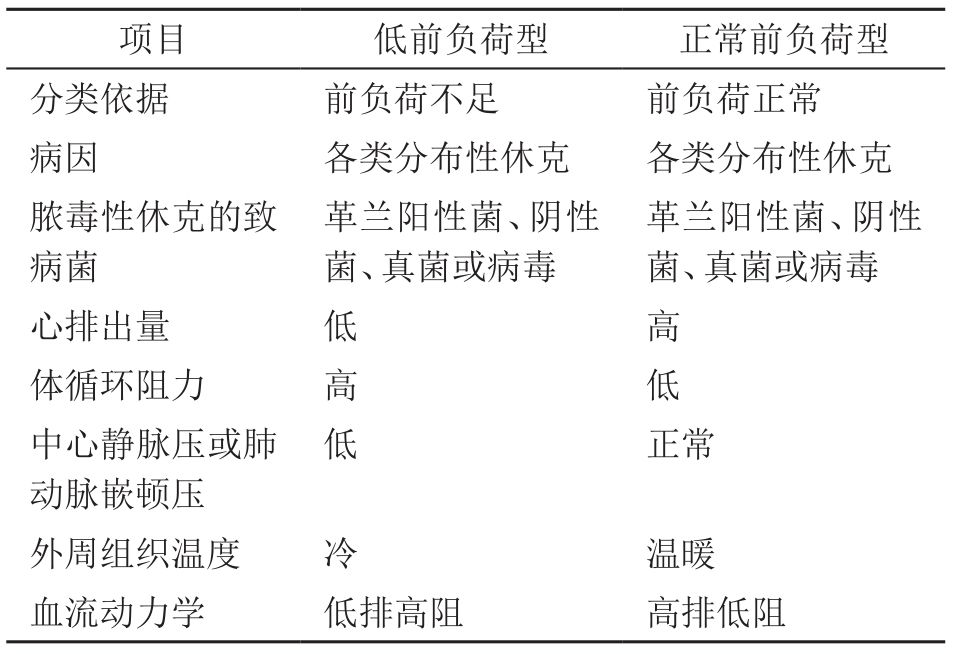
\includegraphics[width=3.25in,height=2.16667in]{./images/Image00084.jpg}
\end{table}

脓毒性休克病例诊断需重视以下几个方面:

\subsubsection{临床表现特点}

\paragraph{感染史}

脓毒性休克常有严重感染基础,尤其注意急性感染、近期手术、创伤、器械检查以及传染病流行病史。当有广泛非损伤性组织破坏和体内毒性产物的吸收亦易发生脓毒性休克。临床表现有寒战、高热、多汗、出血、栓塞、各器官功能减退等。

\paragraph{脑}

脑组织耗氧量很高,对缺氧特别敏感,轻者烦躁不安,重者昏迷抽搐,但脑血管舒缩范围较小,其血流灌注主要取决于供应脑的动静脉血压差。休克早期脑血管代偿性舒张,故脑灌注尚能维持,当休克加重血压明显下降,脑灌注不良,即可产生脑水肿,进一步加重脑灌注不足。患者意识可反映中枢神经系统微循环血流灌注量减少情况,但酸碱、水电解质失衡和代谢产物积蓄对意识有一定影响。临床上休克早期表现为烦躁不安,以后转为抑郁淡漠,晚期嗜睡昏迷。

\paragraph{皮肤}

能反映外周微循环血流灌注情况,所以注意检查皮肤色泽、温度、湿度,有条件可监测血液温度、肛门直肠温度和皮肤腋下温度之差,正常情况各差0.5~1℃,如大于2~3℃则提示外周微血管收缩,皮肤循环血流灌注不足。临床上根据四肢皮肤暖冷差异又可分为“暖休克”和“冷休克”,两者之比较见表\ref{tab20-2}。

\begin{table}[htbp]
\centering
\caption{暖休克与冷休克的比较}
\label{tab20-2}
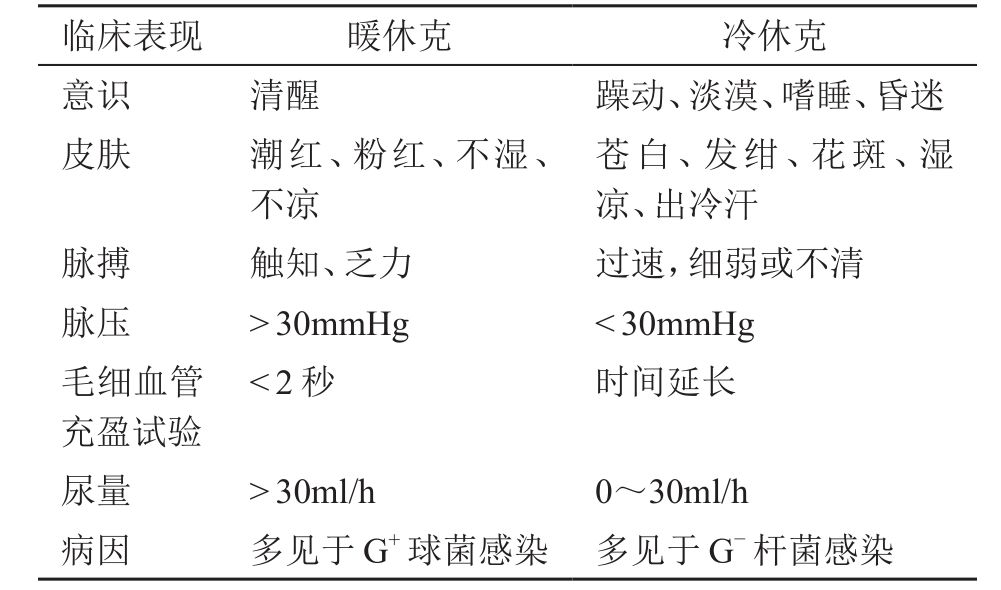
\includegraphics[width=3.32292in,height=1.95833in]{./images/Image00085.jpg}
\end{table}

\paragraph{肾}

肾脏血流量很大,正常达1000~1500ml/min,占全身血流量的25\%,休克时血流产生重新分配,出现肾小动脉收缩,肾灌注量减少,造成少尿或无尿,肾缺血又引起肾小管坏死,影响尿液的浓缩和稀释及酸化功能,出现低比重尿(正常1.010~1.020)、尿pH
>
5.5,提示肾曲小管缺损,存在碳酸氢钠渗漏或远曲小管分泌H\textsuperscript{+}
障碍。

\paragraph{肺}

氧分压(PaO\textsubscript{2} )、氧饱和度(SaO\textsubscript{2}
)和呼吸改变是脓毒性休克时肺功能减退的可靠指标,主要表现在呼吸急促、PaO\textsubscript{2}
和SaO\textsubscript{2}
下降,皮肤和口唇发绀等缺氧表现,其原因有三:①肺泡微循环灌注存在而有通气障碍如肺泡萎陷、肺间质和肺泡水肿、肺炎症等;②肺泡通气良好而有灌注障碍,如回心血量少,心排量降低,肺动脉痉挛,肺微循环栓塞等造成肺血流灌注减少;③肺泡微循环和通气均有障碍。临床常表现为ALI和ARDS。

\paragraph{心脏}

由于细菌毒素作用,常发生中毒性心肌炎;由于细胞线粒体、溶酶体和代谢障碍酸中毒对心肌产生抑制作用,心肌收缩力减退,心排血量减少,血压下降、脉压小、冠状动脉灌注不足,心肌缺血、缺氧等造成心功能损害,急性心力衰竭和心律失常发生,进一步加重休克。

\paragraph{胃肠和肝}

在脓毒性休克时胃肠和肝可发生充血、水肿、出血和微血栓形成,消化道常发生应激性溃疡、糜烂、出血。肝细胞因内毒素和缺血缺氧而发生坏死,使肝功能各项酶、胆红素和血糖升高。

\paragraph{造血系统}

由于内毒素作用,常发生造血抑制和微血栓形成,结果造成血小板和各项凝血指标下降,临床出现DIC。

\paragraph{甲皱循环与眼底改变}

脓毒性休克时常因微血管痉挛造成甲皱毛细血管袢数目减少,周围渗出明显,血流呈断线、虚线或淤泥状,血色变紫,眼底检查小动脉痉挛,小静脉淤血扩张,动静脉比例由正常2∶3变为1∶2或1∶3,严重时有视网膜水肿,颅内压增高者可出现视乳头水肿。

\subsubsection{血流动力学变化特点}

常采用Swan-Ganz导管热稀释法或冷稀释法及非创伤性阻抗法测定血流动力学改变。

\paragraph{动脉血压与脉压}

在脓毒性休克情况下,上臂袖带式听诊法常出现听不清,无法了解血压真实数值,故主张桡动脉或股动脉插管直接测压法,当收缩压下降到80mmHg以下或原有高血压者下降20\%即患者的基础血压值降低30mmHg以下者,应认为血压已降低,组织微循环血液出现灌流减少,临床上可诊断为休克。脉压大小与组织血液灌注紧密相关,加大脉压有利改善组织供血供氧。一般要求维持收缩压在80mmHg、脉压>
30mmHg以上。

\paragraph{中心静脉压(CVP)}

主要反映回心血量与右心室搏血能力,有助于鉴别心功能不全还是血容量不足引起的休克,对决定输液的量和质,对选用强心、利尿或血管扩张剂均有较大指导意义。正常CVP为6~12cmH\textsubscript{2}
O,它与右心室充盈压成正比,在无肺循环或右室病变情况下,亦能间接反映右心室舒张末压和心脏对输液的负荷能力。

\paragraph{肺动脉楔压(PAWP)与左心房平均压}

与左心室舒张末压密切相关,在无肺血管和二尖瓣病变时测定PAWP,能反映左心室功能,对估计血容量,掌握输液速度和防止肺水肿等是一个很好指标。其正常值5~16mmHg。

\paragraph{心排血量(CO)}

反映心脏泵功能的一项综合指标,受心率、前负荷、后负荷及心肌收缩性等因素的影响。其正常值4~8L/min。

\paragraph{脉搏和静脉充盈情况}

脓毒性休克早期脉呈细速(120~140次/分),在休克好转过程中脉搏强度的恢复较血压早。休克时需观察静脉充盈程度,当静脉萎陷,且补液穿刺有困难,常提示血容量不足,而静脉充盈过度则反映心功能不全或输液过多。

临床上根据血流动力学变化,将脓毒性休克分为三个类型:①低排高阻型:常由严重G\textsuperscript{−}
杆菌感染而释放类脂多糖蛋白复合体,刺激机体防御功能分泌大量儿茶酚胺,引起微动脉及微静脉痉挛,动静脉短路开放,回心血量减少,同时毒素和代谢产物对心肌抑制,造成心排血量降低;②高排低阻型:常由G\textsuperscript{+}
球菌严重感染引起机体组胺释放β受体兴奋使心排量增加,外周血管扩张阻力减低,血压下降所形成。③低排低阻型:在休克晚期进入微循环衰竭期,血管平滑肌麻痹而扩张,心功能衰竭,排血量又减少,各重要脏器损伤,并发症相继出现,常属濒死阶段。

\subsubsection{实验室检查}

1.血象
脓毒性休克其白细胞总数多升高,中性粒细胞增加,核左移。但如感染严重,机体免疫抵抗力明显下降时,其白细胞总数可降低。血细胞比容和血红蛋白增高,提示血液浓缩。并发DIC时,血小板进行性下降。

2.尿和肾功能
当有肾衰竭时尿比重由初期偏高转为低而固定,血肌酐和尿素氮升高,尿与血的肌酐浓度之比<
1∶5,尿渗透压降低,尿/血浆渗透压的比值< 1.5,尿钠排出量>
40mmol/L,尤其警惕尿量多比重低,尿素氮、肌酐增高的“非少尿性肾衰”。

3.血气分析 常有低氧血症、代谢性酸中毒、而PaCO\textsubscript{2}
早期由于呼吸代偿而可轻度下降呈呼吸性碱中毒,晚期出现呼吸性酸中毒。

4.血清电解质 血钠和氯多偏低,血钾高低不一。

5.出凝血各项指标 多有异常改变,动态监测提高DIC诊断警惕性。

6.动脉血乳酸浓度
是反映休克程度和组织灌注障碍重要指标,需2~4小时监测一次。

7.寻找病原体,有利于去除病因。

\subsubsection{诊断注意事项}

笔者提出如下注意点供临床参考:

\paragraph{意识状态}

意识变化随血压变化出现烦躁转入昏迷,但需因人而异,老年患者有动脉硬化,即使血压下降不明显,亦可出现明显意识障碍,反之体质好,脑对缺氧耐受性高,虽然血压测不到,其神志仍可清醒。

\paragraph{血压}

是诊断休克的一项重要指标,但在休克早期,由于交感神经兴奋,儿茶酚胺释放过多,可以造成血压“假性”升高,此时如使用降压药,将会引起严重后果。

\paragraph{尿量}

既反映肾微循环血流灌注量,亦可间接反映重要脏器血流灌注情况,当血压维持在80mmHg,尿量>
30ml/h,表示肾灌注良好。当冷休克时,袖带法血压听不清,而尿量尚可时,表示此血压尚能维持肾灌注,反之使用血管收缩剂,血压虽在90mmHg以上,但四肢皮肤湿冷,无尿或少尿,同样提示肾和其他脏器灌注不良,预后差(表\ref{tab20-3}和表\ref{tab20-4})。

\paragraph{肾功能}

肾功能判断不仅注意尿量,而且尿比重和pH以及血肌酐和尿素氮水平进行综合分析,不要被单纯尿量所迷惑,注意对非少尿性急性肾功能衰竭的鉴别,此时尿量可超过1000ml/d,但尿比重低且固定,尿pH上升,提示肾小管浓缩和酸化功能差,血清肌酐和尿素氮上升,表示肾脏功能不佳,应予注意识别。

\paragraph{低氧}

对于低氧血症和ARDS诊断,应有足够认识。由于低氧血症原因未能很好寻找,救治措施不力,产生一系列代谢紊乱,结果出现不可逆休克。作者体会尽早行机械辅助通气,纠正低血氧。但要注意排除非ARDS(血气胸、连枷胸反常呼吸、气道堵塞和严重充血性心力衰竭等)引起的严重低氧血症。

\paragraph{血糖}

休克时血糖水平经常较高,此因感染性休克时交感神经兴奋,生糖激素释放,肝功能受损,胰岛功能减退,外源性葡萄糖补充等影响,造成继发性高血糖,对细菌、真菌生长创造了很好条件,同时高血糖又带来血液高渗,尤其对中枢神经损害和血管反应性进一步下降,休克加剧。

\paragraph{心率判断}

正常心率60~100次/分,但脓毒性休克时机体处于高代谢状态,同时细菌毒素和代谢产物对心脏作用,故心率代偿性增快常在100次/分以上,一旦下降至60~70次/分钟,常预示心脏失代偿而即将停止跳动,不要误认为心功能改善。

\paragraph{血清电解质变化}

需要准确判断与分析。由于脓毒性休克代谢性酸中毒,细胞释放K\textsuperscript{+}
,故血清钾有时很高且难以下降,但大剂量利尿剂、脱水剂和胃肠减压等影响,血清钾均可下降;又由于体液丧失,血液浓缩,使血清钾相对升高,而此时细胞内可以存在严重低钾,故应结合血生化、心电图和临床综合分析判断。脓毒性休克时,常存在镁、锌、铜、磷等降低,尤其镁的补充对MODS防治可获裨益。

\paragraph{酸碱失衡鉴别}

脓毒性休克组织缺血、缺氧、代谢性酸中毒是酸碱失衡基础,但由于呼吸深快的代偿作用,出现代谢性酸中毒+呼吸性碱中毒,血pH可以在正常范围,一旦呼吸抑制出现代谢性酸中毒+呼吸性碱中毒,病情加剧。当同时合并低氯、低钾又产生代谢性碱中毒时,血气分析判断更为复杂,为三重性酸碱失衡,应结合临床进行鉴别。

\begin{table}[htbp]
\centering
\caption{组织灌流检查}
\label{tab20-3}
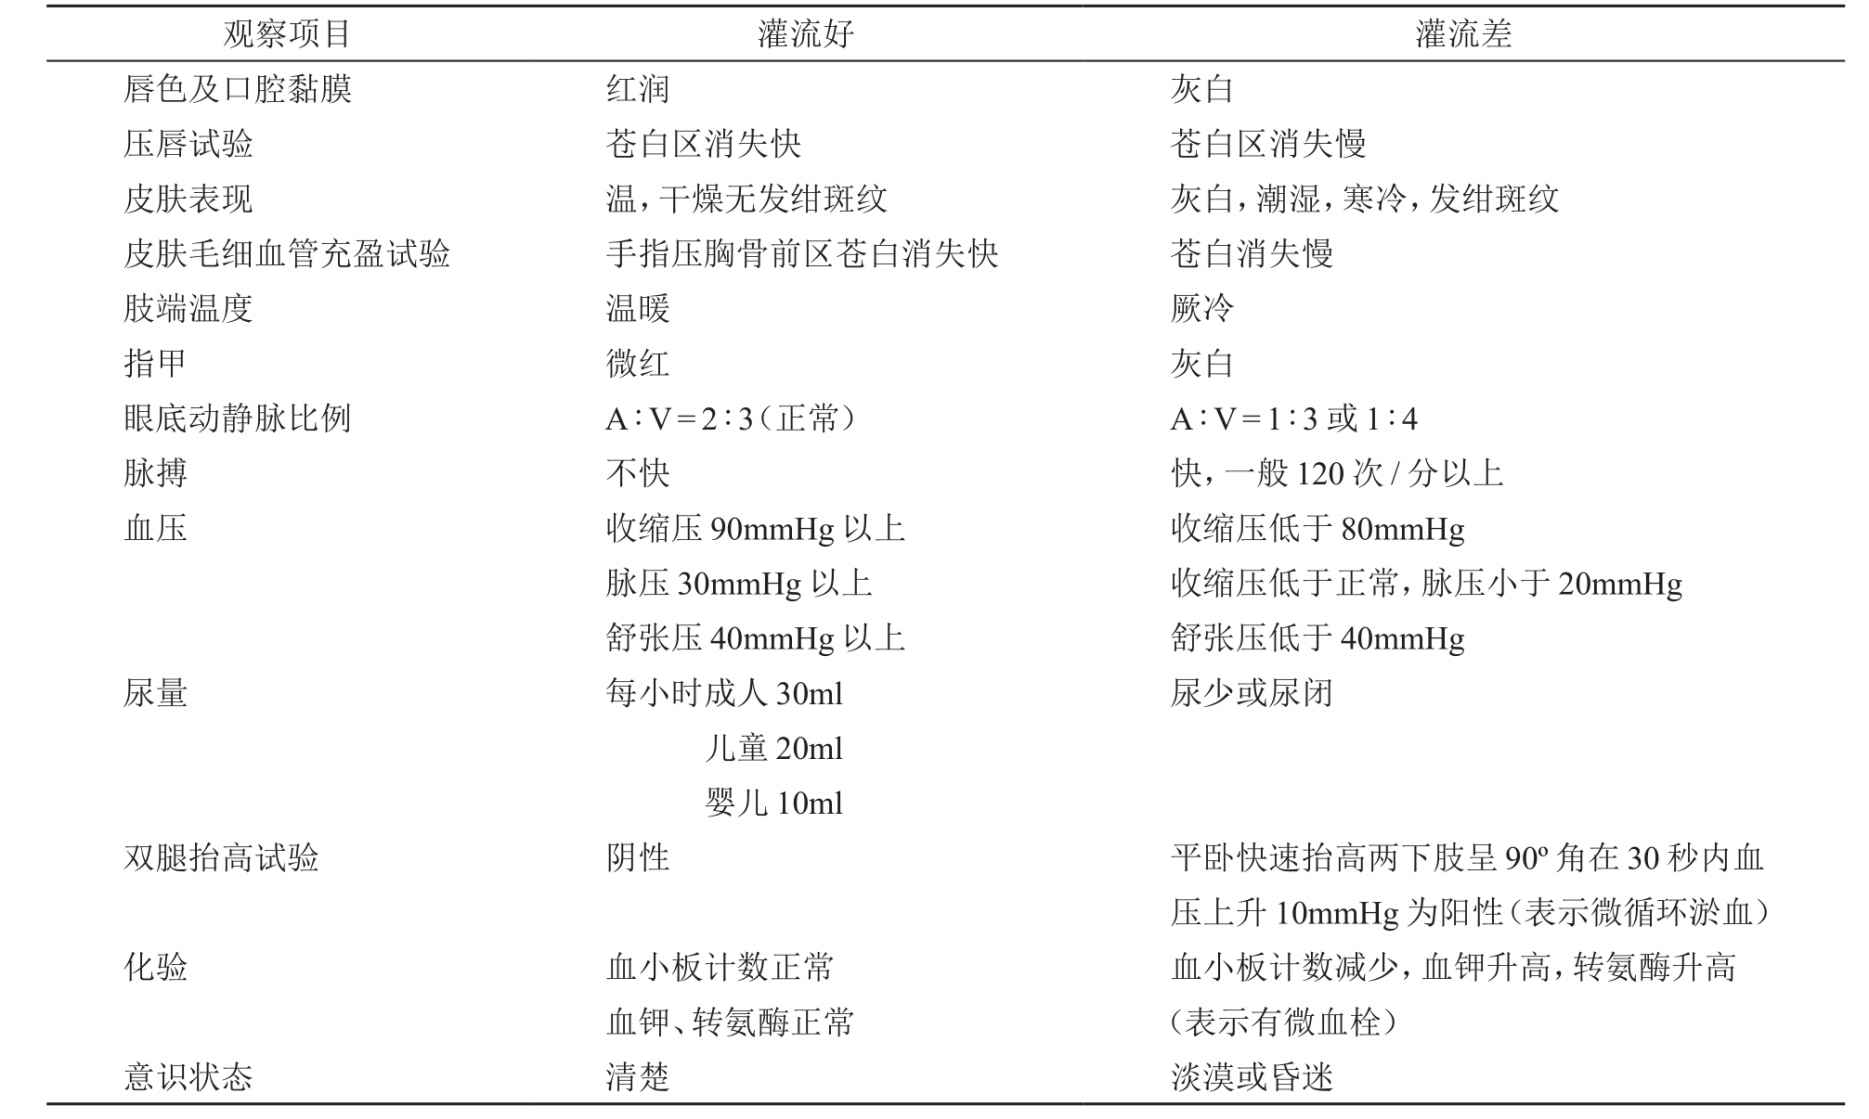
\includegraphics[width=6.69792in,height=4.01042in]{./images/Image00086.jpg}
\end{table}

\begin{table}[htbp]
\centering
\caption{休克程度的鉴定}
\label{tab20-4}
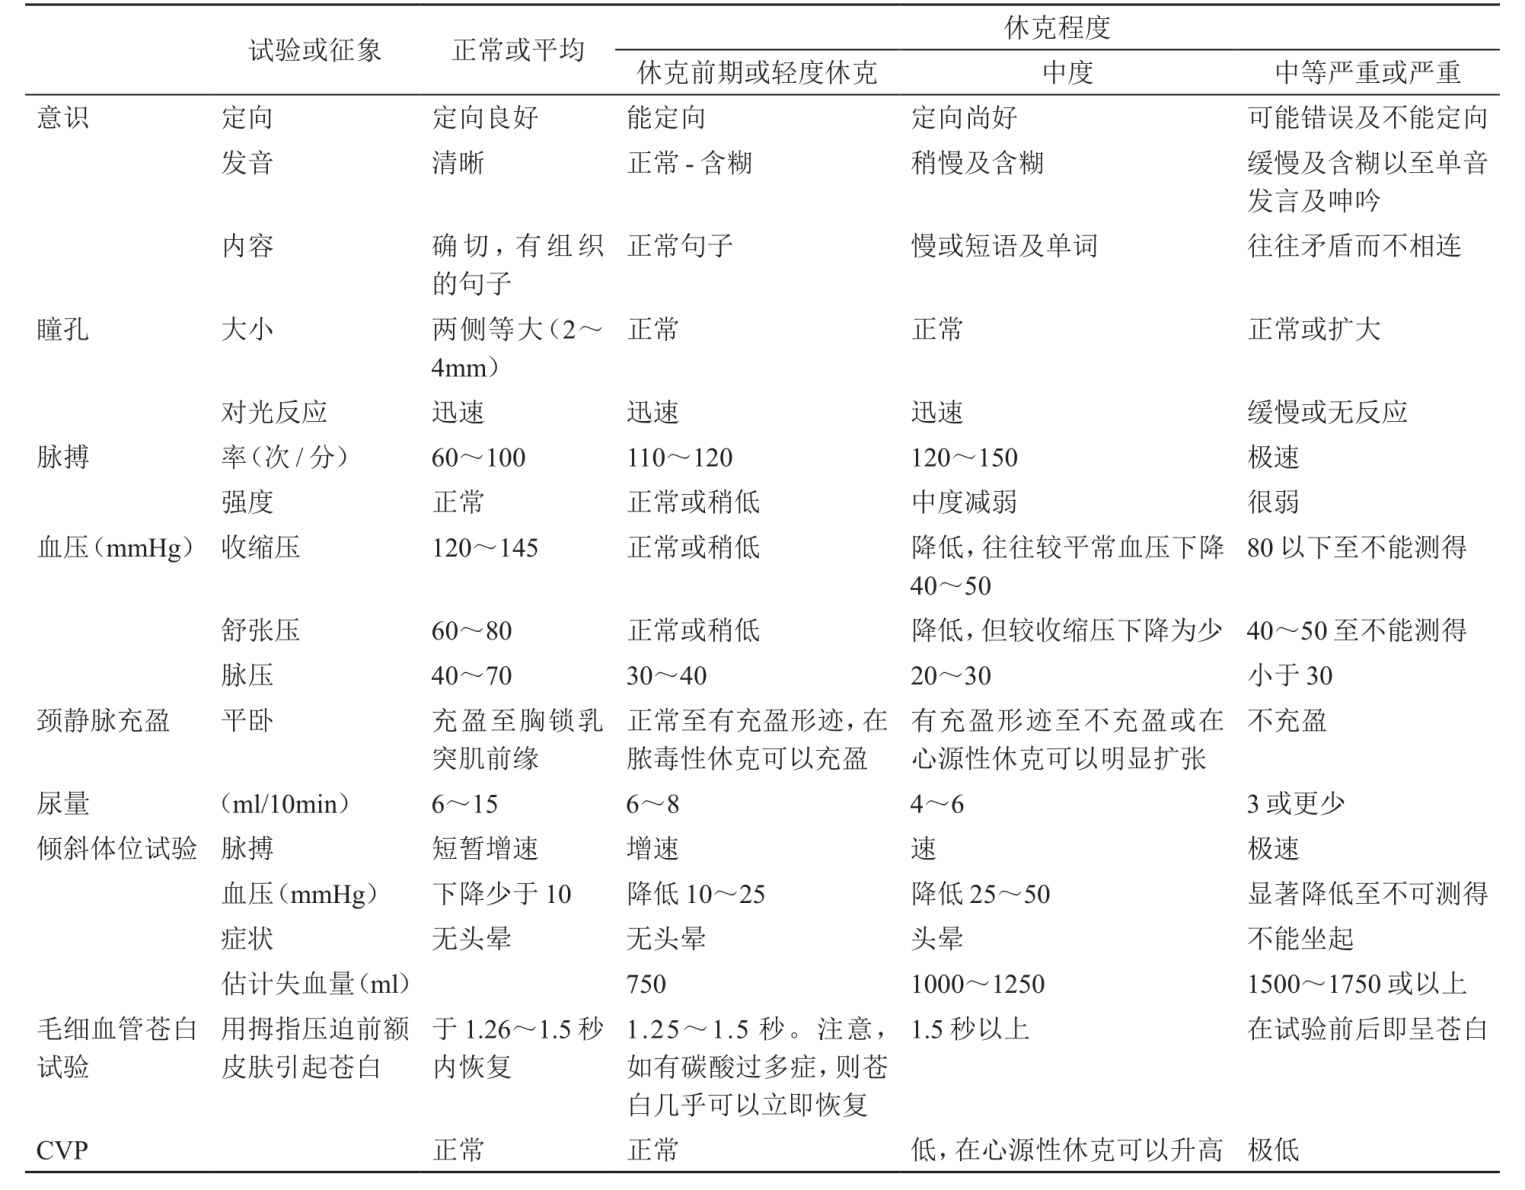
\includegraphics[width=6.66667in,height=5.19792in]{./images/Image00087.jpg}
\end{table}

\paragraph{注意二重感染}

鉴于抗生素使用广泛,且剂量大,常可掩盖局部严重感染征象,又由于抗休克时采用大剂量激素,容易并发真菌感染,注意血、尿、粪、痰和口腔检查真菌病原体,争取早发现,早处理。

\subsection{治疗}

\subsubsection{早期目标治疗(EGDT)}

患者由于脓毒症导致的休克定义为组织的低灌注(表现为经过最初的液体复苏后持续低血压或者血乳酸浓度≥4mmol/L),此时应当进行早期复苏,并且应当在确定存在组织低灌注第一时间进行而不是延迟到患者入住ICU以后实施。在进行早期复苏的最初6小时内,由脓毒症导致的休克所存在的组织低灌注复苏目标包括以下方面:①中心静脉压(CVP):8~12mmHg;②平均动脉压(MAP):≥65mmHg;③尿量:≥0.5ml/(kg•h);④中心静脉(上腔静脉)氧饱和度(ScvO\textsubscript{2}
)或者混合静脉氧饱和度(SvO\textsubscript{2} )分别≥70\%或者≥65\%。

脓毒性休克在最初6小时复苏过程中,虽然经过液体复苏CVP已经达到了目标,但是对应的ScvO\textsubscript{2}
与SvO\textsubscript{2}
没有达到70\%或者65\%,可以为患者输入浓缩红细胞达到血细胞比容≥30\%同时(或者)输入多巴胺(最大剂量为20μg/kg•min)来达到目标。

\subsubsection{控制感染}

抗感染治疗是救治脓毒性休克主要环节。在无明确病原菌前,应经验性选择抗感染治疗方案,根据原发病灶和临床表现,推测最可能的致病菌,选用一种或者更多的强力、广谱抗生素以对抗所有可能的病原微生物{[}细菌和(或)真菌{]},并且要有足够的药物浓度可以渗透到可能导致脓毒症的感染病灶中去。要尽可能快的寻找病因并诊断或者排除诊断,所有表现为脓毒性休克的患者,要对其感染灶的病原学控制情况做出评估,尤其是当患者有脓肿引流或者有局部感染灶,感染后坏死组织清创,摘除可引起感染的医疗工具等。

对于抗生素应用有主张从一代头孢菌素开始逐步升级至三、四代。但脓毒性休克的发生常来势凶猛,病情危急,且细菌的病原菌不明,常带来治疗困难,故按“降阶梯治疗”实行“猛拳出击全面覆盖”原则,可选用碳青霉烯类(美平、泰能等),疗效较高,应尽早应用。

确认脓毒性休克后,应在1小时之内尽早静脉使用抗生素进行治疗。在进行抗生素应用之前留取合适的标本,但是不能为留取标本而延误抗生素的使用。如果患者现有的临床症状被确定为非感染性因素引起,应停止抗生素治疗以减少患者可能被抗生素耐药细菌引起感染和与药物相关的副作用风险。

\subsubsection{液体复苏}

脓毒性休克时均有血容量不足,推荐用天然/人工的胶体或晶体液进行液体复苏。目前没有证据支持某种液体优于其他种类液体。目前实验表明使用白蛋白等同于晶体液。一些关于ICU患者的小规模研究的Meta分析表明晶体和胶体复苏效果没有差异。要达到同样的治疗目标时,晶体液量要明显多于胶体液量,但晶体液更便宜。

液体复苏的初始治疗目标是使CVP至少达到8mmHg(机械通气患者需达到12mmHg)。对怀疑有血容量不足的患者进行液体冲击时,在开始的30分钟内要至少用1000ml的晶体液或300~500ml的胶体液。当只有心脏充盈压(CVP或者肺动脉楔压)增加而没有血流动力学改善时,才应该降低补液速度。

\subsubsection{血管活性药的应用}

使用血管活性药物使平均动脉压保持在≥65mmHg。即使在低血容量还没有得到纠正时,就该使用血管加压类药物,使MAP达到65mmHg以上,以保证低血压时能维持组织灌注。另外,在达到MAP治疗目标时应该考虑到患者既往基础病。

脓毒性休克患者推荐将去甲肾上腺素或多巴胺作为纠正脓毒性休克时低血压的首选血管加压药物。不推荐将肾上腺素、去氧肾上腺素或抗利尿激素作为脓毒性休克的首选血管加压药物。如果去甲肾上腺素或多巴胺效果不明显时可以首选肾上腺素。不推荐将低剂量的多巴胺作为肾脏保护药物。随机临床试验和Meta分析在比较低剂量多巴胺和安慰剂的作用时,没有发现差异。因此,目前尚无可用数据支持低剂量多巴胺可以维持肾功能。在出现心脏充盈压升高心输出量降低,出现心肌功能障碍时,应该静脉滴注多巴酚丁胺,但是反对使用它来增加心指数达超常水平,研究发现使用多巴酚丁胺将严重脓毒症患者的氧输送提高到超常水平并没有益处。

笔者认为冷休克低排高阻情况联合使用血管活性药与血管扩张剂常可获裨益。由于脓毒性休克晚期是血管痉挛收缩,故加用血管扩张剂是合理的,它不仅解除微动脉痉挛,而且有降低心脏前后负荷,解除支气管痉挛,有利通气改善,有利于恢复有效循环血量及组织灌注,使组织代谢酸性产物进入血液循环,从而得到及时纠正,达到消除休克之目的。使用血管扩张剂注意点:①在扩容基础上,其有效血容量得到充分补充情况下可加用血管扩张剂;②剂量应逐步升与降,防止机体不适应和反跳现象;③注意首剂综合征发生,有的患者对某种血管扩张剂(如哌唑嗪等)特别敏感,首次用后产生严重低血压反应,故药物种类和剂量需因人而异;④血管扩张剂单一长期应用可产生“受体脱敏”现象,对药物产生不敏感性,故应予更换。莨菪类药物在脓毒性休克救治上为我国首创。纳洛酮治疗脓毒性休克已获得成功,该药可阻断β内啡肽等物质的降压作用,因而使血压回升,同时有稳定溶酶体膜,降低心肌抑制因子的作用,使心排量增加。中药丹参、川芎等具有使微血管淤滞或缓慢流动的血细胞加快流速,降低血液黏度,开放毛细血管网,扩张微血管,疏通微循环,此外尚有抗凝、调整纤溶和清除氧自由基等作用,达到活血化淤改善微循环防治DIC的作用。

\subsubsection{纠正酸中毒}

纠正酸中毒可增强心肌收缩力,恢复血管对血管活性药物的反应性,防止DIC的发生。根本措施在于改善组织的低灌注状态。缓冲碱主要起治标作用,且血容量不足时,缓冲碱的效能亦难以充分发挥。首选的缓冲碱为5\%碳酸氢钠,次为11.2\%乳酸钠(肝功能损害者不宜用)。三羟甲基氨基甲烷(THAM)适用于需限钠患者,因其易透入细胞内,有利于细菌内酸中毒的纠正;其缺点为滴注溢出静脉外时可致局部组织坏死,静滴速度过快可抑制呼吸、甚至呼吸停止。此外,尚可引起高钾血症、低血糖、恶心呕吐等。当pH≥7.15时,不推荐使用碳酸氢盐改善血流动力学状态或减少升压药应用。

\subsubsection{肾上腺皮质激素}

糖皮质激素具有抗过敏、抗炎、抗毒素、抗休克等作用,经临床大量观察证明其可降低脓毒血症、脓毒性休克病死率。但只建议在血压对于液体复苏和血管加压药治疗不敏感时应用静脉肾上腺皮质激素。且如果可以使用氢化可的松不推荐使用地塞米松,而氢化可的松不应大于300mg/d。当不再需要血管升压类药物时,即应停用皮质激素治疗。

\subsubsection{重组人类活化蛋白C(rhAPC)}

rhAPC具有促进纤维蛋白溶解、抑制血栓形成及抑制白细胞活化的特性。脓毒性休克患者体内内源性活化蛋白C水平显著下降,并有研究表明rhAPC的补充可降低脓毒性休克的病死率,故国外指南建议脓毒症诱导的器官功能不全伴有高死亡危险(大多数APACHEⅡ≥25或多器官功能不全)的成年患者,如果没有禁忌证,应接受rhAPC治疗。低死亡危险严重脓毒症成年患者(APACHEⅡ<
20或一个器官衰竭),不予rhAPC治疗。

\subsubsection{血液制品}

一旦发现成人组织低灌注难以减轻,如心肌缺血、严重低氧血症、急性出血、发绀型心脏病或乳酸酸中毒,推荐当血红蛋白下降低于7.0g/dl(70g/L)时输注红细胞,使血红蛋白维持在7.0~9.0g/dl(70~90g/L)。在没有出血或有计划的侵入性操作时,如果凝血实验正常,不建议用新鲜冷冻血浆。新鲜冷冻血浆对于危重患者预后的影响,尽管没有临床研究评价,但当证实有凝血因子缺乏(凝血酶原时间、国际标准化比率或部分凝血活酶延长)、活动性出血或外科手术或侵入性操作前,推荐输注新鲜冷冻血浆。当血小板计数<
5 × 10\textsuperscript{9}
/L,无论是否有出血,都推荐输注血小板。当血小板计数5 ×
10\textsuperscript{9} ~30 × 10\textsuperscript{9}
/L并且有明显出血危险时,可以考虑输注血小板。外科手术或侵入性操作特别需要血小板计数≥50
× 10\textsuperscript{9} /L。

\subsubsection{血糖控制}

对进入重症监护病房后已经初步稳定的重症脓毒症合并高血糖患者,应使用强化静脉胰岛素治疗来控制血糖,使血糖控制在8.33mmol/L(150mg/dl)以下。所有接受静脉胰岛素治疗的患者都可以用葡萄糖作为热量来源,每1~2小时监测一次血糖,直到血糖和胰岛素用量稳定后可每4小时监测一次。多项研究显示,强化静脉胰岛素治疗,血糖控制可减少ICU死亡率、减少器官功能障碍及住ICU时间。但使用Leuven方案强化胰岛素治疗发生低血糖的风险是传统经验治疗的3倍左右。因此,虽然主张积极控制高血糖,但也需警惕低血糖的发生。

\subsubsection{脓毒性休克的支持治疗}

\paragraph{心功能不全的防治}

重症休克和休克后期病例常并发心功能不全,乃因细菌毒素、心肌缺氧、酸中毒、电解质紊乱、心肌抑制因子、肺血管痉挛、肺动脉高压和肺水肿加重心脏负担,及输液不当等因素引起。老年人和幼儿尤易发生,可预防应用毒毛旋花苷或毛花苷丙。出现心功能不全征象时,应严重控制静脉输液量和滴速。除给予快速强心药外,可予血管舒张剂,但必须与去甲肾上腺素或多巴胺合用以防血压骤降。大剂量肾上腺皮质激素有增加心搏血管和降低外周血管阻力、提高冠状动脉血流量的作用,可早期短程应用。同时给氧、纠正酸中毒和电解质紊乱,并给能量合剂以纠正细胞代谢失衡状态。

\paragraph{维持呼吸功能、防治ARDS}

肺为休克的主要靶器官之一,顽固性休克常并发呼吸功能衰竭。此外脑缺氧、脑水肿等亦可导致呼吸衰竭。休克患者均应给氧,经鼻导管(4~6L/min)或面罩间歇加压输入。吸入氧浓度以40\%左右为宜。必须保持呼吸道通畅。在容量补足后,如患者神志欠清、痰液不易清除、气道有阻塞现象时,应及早考虑作气管插管或切开并行辅助呼吸,并清除呼吸道分泌物,注意防治继发感染。对吸氧而不能使PO\textsubscript{2}
达满意水平(>
9.33~10.7kPa)、间歇正压呼吸亦无效的A-V短路开放病例,应及早给予呼气末正压呼吸(PEEP),可通过持续扩张气道和肺泡、增加功能性残气量,减少肺内分流,提高动脉血氧分压、改善肺的顺应性、增高肺活量。除纠正低氧血症外,应及早给予血管解痉剂以降低肺循环阻力,并应正确掌握输液、控制入液量。对于ALI/ARDS患者进行机械通气,应设定6ml/kg的潮气量;设定初始平台压上限≤30cmH\textsubscript{2}
O,评估气道压力时应考虑胸壁顺应性因素;允许PaCO\textsubscript{2}
高于正常水平,如需要,可减少平台压和潮气量;设置PEEP防止呼气末肺泡塌陷;对需要保持可能对机体造成潜在损伤水平较高FiO\textsubscript{2}
或气道高压的ARDS患者,只要不存在体位改变的风险,应考虑使用侧卧体位;除非禁忌,机械通气患者应取半卧位,床头抬高30°~45°。

\paragraph{肾功能的维护}

休克患者出现少尿、无尿、氮质血症等时,应注意鉴别其为肾前性或急性肾功能不全所致。在有效心搏血量和血压回复之后,如患者仍持续少尿,可行液体负荷与利尿试验:快速静滴甘露醇100~300ml,或静注速尿40mg,如排尿无明显增加,而心脏功能良好,则可重复一次,若仍无尿,提示可能已发生急性肾功能不全,应给予肾脏替代治疗。若循环稳定可予血液透析治疗,对血流动力学不稳定患者,CVVH更适宜、方便、安全。

\paragraph{脑水肿的防治}

脑缺氧时,易并发脑水肿,出现神志不清、一过性抽搐和颅内压增高征,甚至发生脑疝,应及早给予血管解痉剂、抗胆碱类药物、渗透性脱水性(如甘露醇)、速尿、头部降温与大剂量肾上腺皮质激素(地塞米松10~20mg)静注以及高能合剂等。

\paragraph{DIC的治疗}

DIC的诊断一经确立后,采用肝素或低分子肝素,并适当输注新鲜血浆、全血及血小板。在DIC后期、继发性纤溶成为出血的主要原因时,可加用抗纤溶药物。

\paragraph{应激性溃疡的防治}

脓毒性休克患者可以使用H\textsubscript{2}
受体阻滞剂或质子泵抑制剂PPI来预防应激性溃疡导致的上消化道出血,但也要考虑到胃内pH升高可能增加呼吸机相关性肺炎的风险。在ICU患者预防应激性溃疡致上消化道出血的收益的研究中,有20\%~25\%的合并脓毒症。这种获益应适用于重症脓毒症及脓毒性休克患者。此外,受益于应激性溃疡预防性治疗的几种情况的患者(凝血功能障碍,机械通气,低血压)经常合并严重脓毒症和脓毒性休克。预防上消化道出血的同时也必须权衡胃内pH升高的潜在的影响,这会增加发生呼吸机相关肺炎的风险。那些上消化道出血风险最大的严重脓毒症患者最能从预防应激性溃疡中获益。

\protect\hypertarget{text00058.html}{}{}

\hypertarget{text00058.htmlux5cux23CHP2-2-4}{}
参 考 文 献

1. 中华医学会重症医学分会
.成人严重感染与感染性休克血流动力学监测及支持指南(草案).中国实用外科杂志,2007,27:7-13.

2. Delling RP,LeveMM,Carlet JM,et al. Surviving Sepsis
Campaign:International guidelines for management of severe sepsis and
septic shock:2008. Crit Care Med,2008,36:296-327.

3.
周荣斌,王新华.从脓毒症基础研究热点展望临床治疗前景.中国急救医学,2009,29(8):674-688

\protect\hypertarget{text00059.html}{}{}

\chapter{心源性休克}

心源性休克(cardiogenic
shock,CS)是指各种原因所致的以心脏泵血功能障碍为特征的急性组织灌注量不足而引起的临床综合征。与其他休克一样,其共同特征是有效循环血量不足,组织和细胞的血液灌注虽经代偿仍受到严重限制,从而引起全身组织和脏器的血液灌注不良。其主要临床表现除有原发性心脏病的表现外,尚伴有血压下降,面色苍白,四肢湿冷和肢端发绀,浅表静脉萎陷,脉搏细弱,全身乏力,尿量减少,烦躁不安,反应迟钝,神志淡漠,甚至昏迷等。

CS最常见的病因为急性心肌梗死(AMI)。狭义上的心源性休克指的是发生于AMI泵衰竭的严重阶段。广义上心源性休克还包括其他原因,如充血性心力衰竭、急性心肌炎、心肌病,乳头肌或腱索断裂、瓣叶穿孔,严重心脏瓣膜病变和严重的心律失常等心脏因素以及心包填塞、张力性气胸等外在阻力因素等。有学者曾将心源性休克分为两大类,即冠状动脉性休克和非冠状动脉性休克。也有主张按病理和临床特点进行分类为心肌坏死后心源性休克和非心肌坏死性心源性休克。GUSTO-1的研究表明AMI并发CS的发生率为7\%,几乎所有的休克都是在发病48小时内发生,并且30天的死亡率高达57\%。总的看来,AMI并发CS的发生率为7\%~10\%,病死率高达50\%~80\%。

\subsection{病因与发病机制}

\subsubsection{病因}

根据致病因素的特点,可以把心源性休克的主要病因归为以下几类:

\paragraph{急性心肌梗死}

CS更常见于ST段抬高性心肌梗死(ST-segment elevation myocardial
infarction,STEMI)患者。目前约5\%~8\%的STEMI患者合并CS,而非ST段抬高性心肌梗死(non-ST-segment
elevation myocardial
infarction,NSTEMI)患者为2.5\%。AMI伴CS患者通常冠状动脉病变严重,约2/3为3支血管病变,20\%为左主干病变,常见于左心室梗死面积大于40\%的患者。约40\%的患者有既往梗死史,对于既往大面积梗死者,即使是小面积再次梗死也可诱发CS。梗死面积扩展或梗死相关动脉再闭塞,非梗死区域心肌代偿失调等,均是迟发性CS的因素。右心室梗死同样是CS的重要原因,分别占GUSTO-1试验和SHOCK登记研究CS患者的20\%和5\%,梗死相关动脉96\%为右冠状动脉,其年龄相对较轻,陈旧性梗死病史相对较少,前壁梗死和多支血管病变相对少见,但病死率与左心室CS相仿,早期血运重建对两者病死率的影响相似。左心室泵衰竭同时伴有右心功能不全,并不进一步增加病死率。包括心室间隔穿孔、乳头肌功能不全或断裂所致的急性二尖瓣反流、心室游离壁破裂等在内的机械并发症,仍是导致CS的重要病因,病死率极高。下后壁梗死,尤其是首次梗死伴CS者,应高度怀疑合并机械并发症。

AMI伴CS的危险因素包括:高龄、前壁梗死、高血压、糖尿病、多支血管病变、既往梗死史和心绞痛史、既往心力衰竭史、STEMI和左束支传导阻滞等。

\paragraph{其他原因}

①终末期心肌病。②急性弥漫性心肌炎。③心肌挫伤或心脏手术后。④感染性休克所致严重心肌抑制。⑤严重心律失常。⑥左室流出道梗阻:主动脉狭窄、肥厚梗阻性心肌病。⑦左室充盈受阻:严重二尖瓣狭窄、左房黏液瘤。⑧瓣膜破裂所致急性二尖瓣反流。⑨急性心肌梗死时部分心源性休克的发生与不恰当的治疗或过度治疗有关,如过量的肾上腺素β受体阻滞药、ACEI、ARB、吗啡、利尿药均可导致低血压和组织低灌注。

\subsubsection{发病机制}

\paragraph{病理生理学}

心源性休克患者的心功能不全往往是由急性心肌梗死或缺血所导致,而心功能不全又会加重心肌缺血的情况,导致恶性循环。当大块心肌缺血坏死并产生泵血功能下降时,每搏输出量及心输出量也将下降。冠状动脉供血主要取决于心脏舒张时冠脉循环与左室内压力的压力梯度,而低血压及心动过速将影响这一压力梯度并导致冠脉供血下降而加重心肌缺血。心室泵功能的下降将进一步降低冠脉灌注压,心室充盈又令心肌需氧量增加,因而加重心肌缺血。心输出量的下降令外周循环灌注下降,进而导致乳酸性酸中毒,进一步降低心肌收缩力。

随着心肌功能的下降,数种代偿机制将被激活,包括交感神经兴奋增加心率及心肌收缩力,肾素-血管紧张素-醛固酮系统(RAAS)的激活致水钠潴留增加前负荷、血管收缩而增加后负荷。这些代偿机制的激活将进一步诱发心源性休克的进展,心率增加及心肌收缩力增加将增加心肌氧需求量及加重心肌缺血,液体潴留、因心动过速及心肌缺血所导致的舒张期充盈过度将导致肺淤血及低氧血症。为维持有效血压水平机体血管收缩,又加重了心肌的后负荷水平并令心肌功能进一步受损及增加心肌氧需求,增加的心肌氧需求量和灌注下降,令心肌缺血加重,以上因素如不能及时进行干预将形成恶性循环而导致死亡(图\ref{fig21-1})。

\begin{figure}[!htbp]
 \centering
 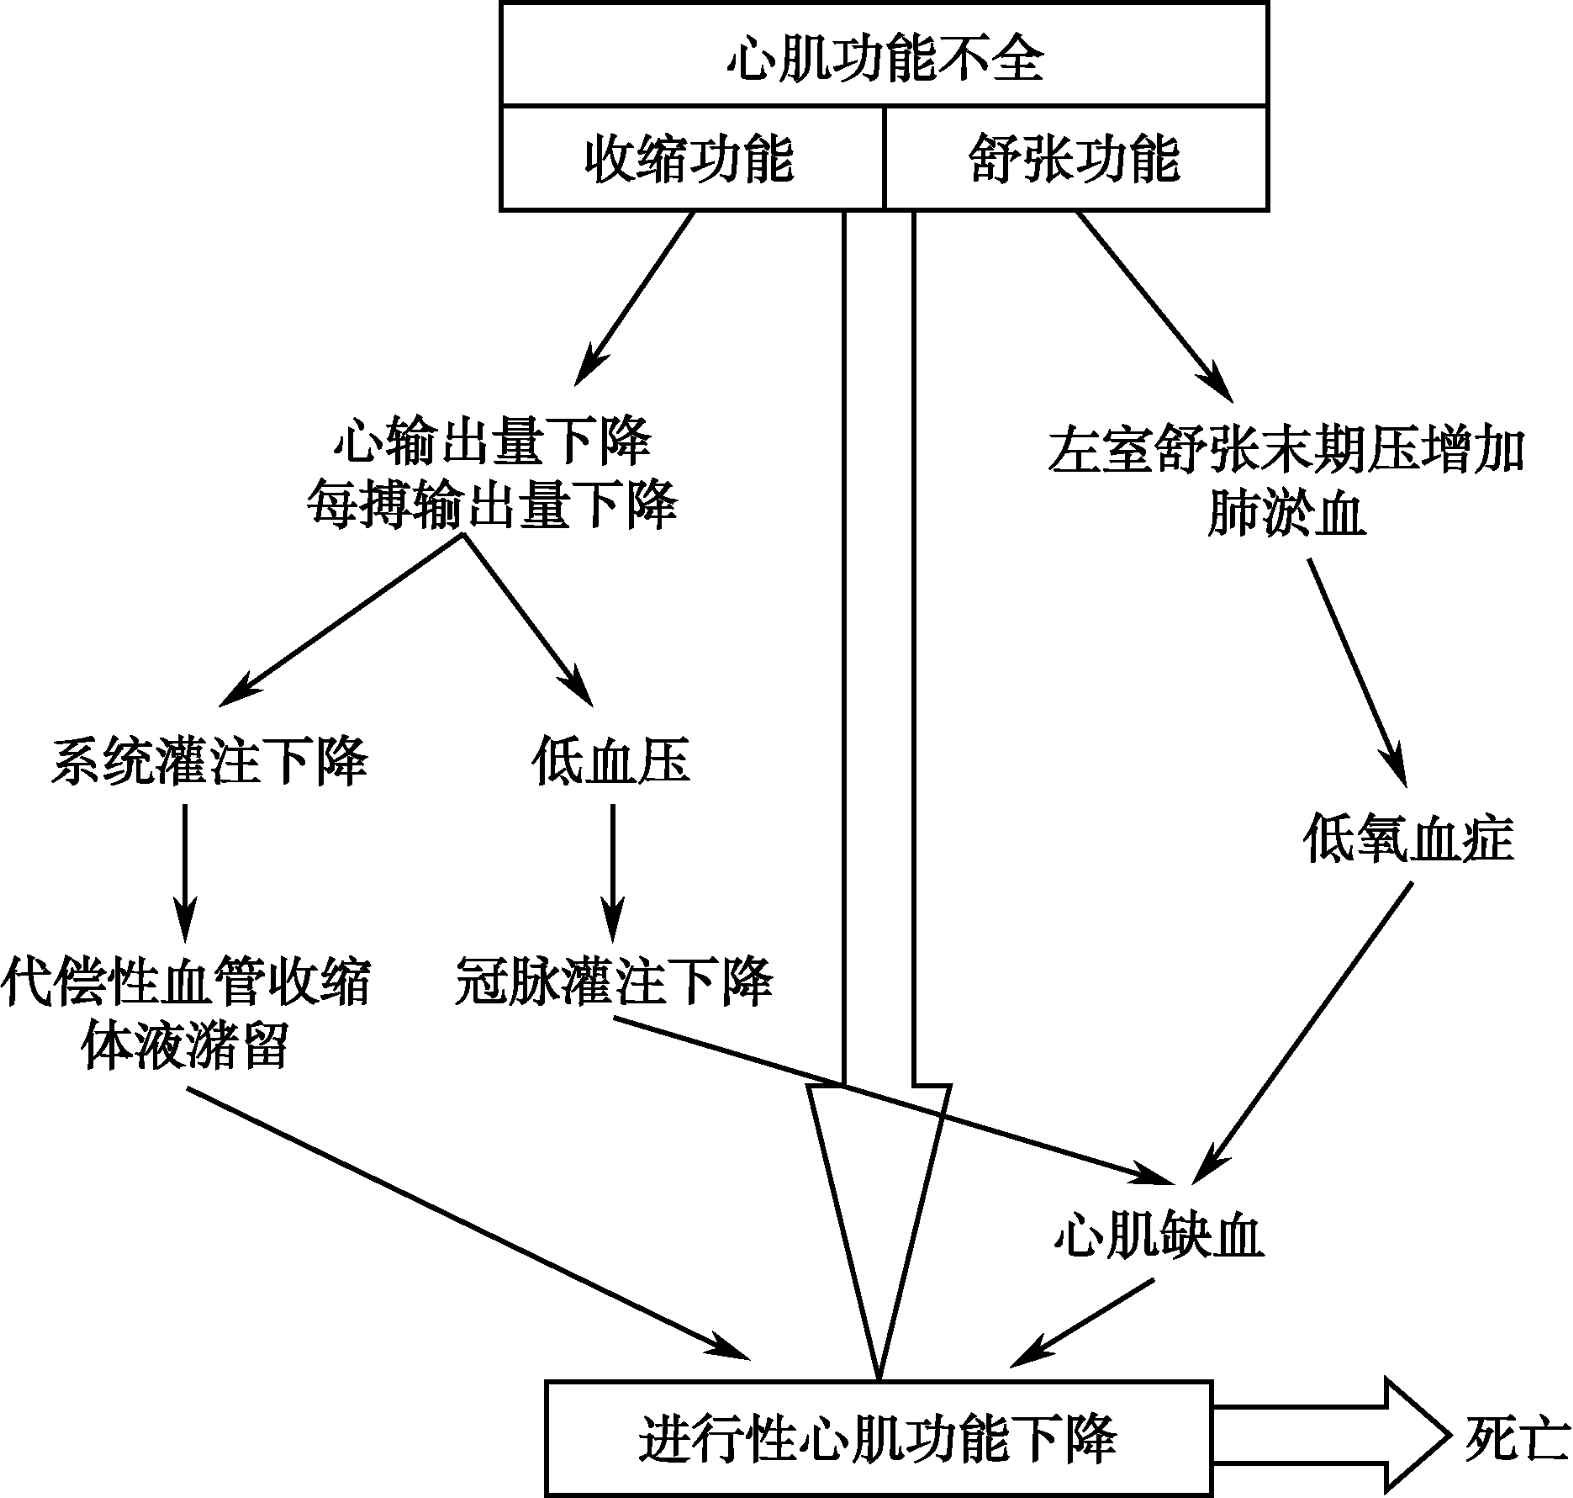
\includegraphics[width=3.11458in,height=2.96875in]{./images/Image00088.jpg}
 \captionsetup{justification=centering}
 \caption{心源性休克的发病机制}
 \label{fig21-1}
  \end{figure} 

另外
,在心肌梗死时大量的非梗死细胞出现可逆性功能丧失是患者在心肌梗死后出现心源性休克的重要因素,而这些细胞的可逆性功能丧失可以归为两类:心肌顿抑及心肌冬眠。心肌顿抑,是指心肌缺血后再灌注但心肌功能未能及时恢复,但最终这部分心肌功能可以完全恢复。心肌缺血后氧自由基损伤、钙离子失衡、肌纤维对钙离子反应性下降等可能参与了心肌顿抑的发生。此外循环中心肌顿抑因子也参与了心肌顿抑时的心肌收缩力下降。心肌顿抑的程度与再灌注前心肌缺血的程度有关。

心肌冬眠则是指在冠脉血流严重下降时心肌细胞功能静息,改善冠脉供血将令冬眠心肌细胞的功能恢复正常。心肌冬眠可以被认为是低灌注的心肌为了恢复血流灌注与心肌功能之间的平衡而降低心肌收缩力,是心肌的一种适应性反应,从而避免心肌缺血及坏死。心肌顿抑及心肌冬眠尽管在概念上及病理生理上截然不同,然而在临床上两者难以完全分开,往往合并存在。通过重建冠脉的血流,恢复心肌供血有助于改善心肌冬眠,而尽早恢复心肌供血及恢复心肌细胞离子平衡也有助于改善心肌顿抑。对于心源性休克患者,血流动力学支持以及尽可能降低心肌细胞坏死是极为重要的治疗措施。

\paragraph{心肌病理}

心源性休克时同时存在收缩与舒张功能不全,对心源性休克患者的临床与病理研究均发现有心肌细胞的进行性坏死。部分患者在入院后出现休克,可能是由于特定梗死血管的再梗阻所导致的梗死扩展、冠脉内栓子的扩散或心肌细胞需氧量增加及冠脉灌注下降等所导致。在梗死灶边缘的心肌细胞对缺血因素更为敏感,有进一步发生坏死的危险,而远离梗死灶的心肌细胞也由于缺血而导致收缩功能下降。

在心源性休克患者,往往观察到多支血管病变,冠脉的储备及自我调节功能下降,低血压及代谢产物堆积将影响非梗死的心肌细胞的收缩功能。心肌缺血时心肌顺应性下降,舒张末期容量负荷增加导致左室舒张末期压增加,而为了维持每搏输出量,左室内血容量代偿性增加,进一步令左室舒张末期压增加,继而导致肺淤血及低氧血症的发生。

瓣膜功能异常也参与了肺淤血的发生过程。由于心肌缺血所致的乳头肌功能不全导致二尖瓣关闭不全,继而导致左房压力负荷增加及肺淤血发生,后负荷降低可以减轻二尖瓣反流水平。乳头肌的完全性破裂将在短时间内迅速导致肺淤血及心源性休克的发生。

\paragraph{细胞病理}

组织低灌注及继发的细胞缺氧将导致葡萄糖无氧酵解,ATP生成减少,细胞内能量储备下降,而糖的无氧酵解又会导致乳酸堆积及细胞性酸中毒,能量不足导致细胞各种能量依赖性的离子通道功能丧失,继而导致跨膜电位的改变,细胞内钠、钙离子堆积,细胞水肿,细胞缺血及钙离子堆积将激活细胞内蛋白酶。严重而持续的心肌缺血将令心肌细胞损伤不可逆转,继而发生一系列改变,如线粒体的水肿、破裂,蛋白变性,染色体破坏,溶酶体破裂等,表现为典型的心肌细胞坏死。

细胞凋亡目前被认为参与了心肌梗死时的心肌细胞数量减少过程。在梗死灶以细胞坏死为主,而在梗死灶边缘区甚至远离梗死灶的心肌,由于缺血及低灌注等因素,可发现心肌细胞凋亡的表现,炎症因子暴发性释放、氧自由基损伤及心肌细胞的机械性拉伸等被认为是心肌梗死时凋亡通路启动的主要启动因素。就细胞凋亡对心肌梗死所起的作用,目前尚未完全明确,但在心肌缺血后再灌注的动物模型中进行抗凋亡治疗能减轻心肌细胞损伤。

除外细胞凋亡过程,目前发现心肌细胞胀亡(oncosis)也是心肌梗死及心肌缺血后再灌注损伤过程中导致梗死灶及邻近细胞迅速坏死的重要机制之一,细胞胀亡往往有外部刺激因素所触发,不同于以细胞缩小为主的凋亡过程。细胞胀亡时,胀亡的细胞胞体肿胀,胞膜通透性增加、完整性破坏,胞浆空泡化,内质网储钙能力下降,线粒体肿胀、嵴结构破坏、呼吸链受阻、ATP缺乏或胞核内染色质聚集成块,然而目前针对细胞胀亡的分子机制尚不明确,线粒体的损伤可能触发细胞发生胀亡,因为细胞凋亡过程需要线粒体产生相应所需的ATP方可完成,而在线粒体损伤的情况下ATP生成不足则相应地触发细胞胀亡;而且由于ATP不足会导致内质网过度释放钙离子,这也是导致细胞胀亡的重要机制之一;ATP的耗竭又会进一步导致细胞膜各种离子泵如Na\textsuperscript{+}
-K\textsuperscript{+}
-ATP酶等的功能丧失,同时细胞膜磷脂发生水解破坏,也进一步加剧细胞损伤及死亡。研究发现在发生缺血坏死的区域,供血供氧相对足够的部分常以凋亡为主,而在缺血缺氧较严重的部分则以胀亡居多;研究指出在ATP耗竭超过80\%~85\%时细胞胀亡就可能发生。

\paragraph{炎症反应机制}

患者发生心源性休克时伴随着更严重的炎症反应。THEROUX等研究观察发现白介素-6
(IL-6)和肿瘤坏死因子-α(TNF-α)异常增高的急性心肌梗死患者,入院时Killip分级为Ⅰ级,数日后发展为心源性休克。IL-6和TNF-α均有抑制心肌收缩力的作用。TNF-α还有损伤血管内皮功能的作用,使冠状动脉血流更趋减少。

\subsection{诊断}

\subsubsection{临床表现特点}

\paragraph{原发病的症状和体征}

如胸闷、胸痛、气促,心脏扩大、心前区抬举感,心律失常、心音遥远、出现第三和(或)第四心音、心脏杂音,颈静脉充盈或怒张,肺部细湿啰音,急性心肌梗死患者有典型的心电图及心肌酶学改变。

\paragraph{血压}

动脉收缩压≤80mmHg,舒张压<
60mmHg,原为高血压患者的收缩压≤90mmHg,或由原水平降低30\%以上。

\paragraph{循环不良体征}

皮肤苍白、发绀或出现花斑,皮肤湿冷,手、足背静脉塌陷,脉搏细速,胸骨部位皮肤指压恢复时间大于2秒等。

\paragraph{意识精神状态改变}

烦躁不安、焦虑、反应迟钝,昏睡甚至昏迷。

\paragraph{其他}

呼吸深快、心动过速(并发缓慢型心律失常者除外)、尿量减少。

\subsubsection{临床评估及辅助检查}

心源性休克是临床急症,需要在休克状态导致不可逆的重要器官损伤前迅速进行评估并尽早开始治疗,准确而迅速的病史采集和体格检查有助于了解、诊断原发病。注意排除低血容量、出血、脓毒血症、肺动脉栓塞、主动脉夹层等。对患者的神志情况、尿量、皮肤状况、肺部啰音等的监测有助于监测病情。

\paragraph{心电图}

心电图检查应该及时进行,可以确立心肌梗死的部位、范围,同时应进行心电监护,评估心率、心律,及时发现各种心律失常。

\paragraph{连续性血压检测}

包括床边无创连续性血压监测及动脉内插管测压,血压监测有助于对病情严重性、预后及治疗效果进行评估。由于休克状态下血管收缩以及各种血管活性药物的使用,无创测压测值往往低于实际值,因此采用动脉内插管测压较准确,多作桡动脉内插管测压。

\paragraph{超声心动图}

超声心电图检查有助于确诊心源性休克并排除其他原因所致的休克,能够反映总体及局部心肌的收缩功能,可以发现乳头肌断裂、急性二尖瓣反流、室间隔破裂或室壁瘤的破裂、心包填塞等。

\paragraph{侵入性血流动力学监测}

侵入性血流动力学监测能够排除血容量不足等情况,对治疗方法的选择、疗效及预后的判断有重要作用。常用指标有:

(1) CVP:CVP < 2cmH\textsubscript{2} O时提示存在血容量不足,CVP
>15cmH\textsubscript{2}
O提示右心功能不全,多数心源性休克患者CVP升高,二尖瓣反流、肺动脉栓塞、慢性阻塞性肺部疾病(COPD)、血容量过高时CVP也会升高。

(2)
LVEDP:LVEDP升高提示左室射血功能障碍及心室顺应性下降,LVEDP越高,提示心源性休克越严重,测定LVEDP可能诱发严重的室性心律失常,常采用测定PCWP来间接反映LVEDP。

(3)
PCWP:心源性休克时PCWP常高于15mmHg,PCWP在18~20mmHg时提示存在轻度肺淤血,21~25mmHg时提示中度肺淤血,26~30mmHg时提示重度肺淤血,31~35mmHg提示出现肺水肿,超过36mmHg提示重度肺水肿。对个别患者,由于左室舒张功能下降,为维持最佳的心室充盈压,PCWP可高于15mmHg。

(4)
RAP:心源性休克患者PCWP升高,但RAP一般仅稍升高或正常,合并右心功能不全或心包填塞时RAP明显升高。

(5) CI、CO、SVR:CI < 2.2L(/min•m\textsuperscript{2}
)提示存在心源性休克,CI < 1.8L(/min•m\textsuperscript{2}
)提示严重的心源性休克,动态观察CI、CO、SVR可以了解心脏收缩功能及体循环血管阻力。

(6)
其他指标:通过右心内导管监测血氧饱和度,在室间隔破裂时由于动静脉血混合右心内血氧饱和度升高;出现巨大的V波提示存在严重的二尖瓣反流;右室心肌梗死时右室充盈压明显升高但PCWP正常甚至下降。

\paragraph{冠脉造影}

进行急诊冠脉造影可以发现致梗死的罪犯血管,有助于判断预后,左前降支或多支病变患者发生心源性休克可能性更大,预后更差,在造影同时进行PTCA或支架植入的重建冠脉血流对治疗有重要作用。

\paragraph{其他指标}

血常规、电解质、心肌酶学、凝血功能等应即时进行检测及动态监测,有助于监测病情,了解心肌梗死程度并指导治疗方案。动脉血气分析可以提示是否存在呼吸功能衰竭。血乳酸水平检测可以反映休克持续的时间及循环障碍的程度。胸部X线拍片可以发现肺水肿等情况。

\subsubsection{诊断标准与病因判断}

\paragraph{休克诊断标准}

1982年2月全国急性“三衰”会议制订的休克诊断试行标准为:①有诱发休克的病因;②意识异常;③脉细速,超过100次/分或不能触及;④四肢湿冷,胸骨部位皮肤指压阳性(指压后再充盈时间>
2秒),皮肤花纹、黏膜苍白或发绀,尿量< 30ml/h或无尿;⑤收缩压<
80mmHg;⑥脉压< 20mmHg;⑦原有高血压者收缩压较原水平下降30\%以上。

凡符合以上①,以及②、③、④中的两项,和⑤、⑥、⑦中的一项者,可诊断为休克。

\paragraph{心肌损伤所致心源性休克的诊断}

CS为心室泵衰竭导致心输出量锐减,出现靶器官的低灌注状态,其核心为心室泵衰竭诱发的血流动力学紊乱伴有组织灌注不足。表现为持续性(超过30分钟)低血压(如收缩压<
80~90mmHg或者平均动脉压低于基线水平30mmHg,或者需要药物或机械支持使血压维持在90mmHg左右)伴有心脏指数(cardiac
index,CI)严重降低{[}无器械支持时< 1.8L/ (min•m\textsuperscript{2}
),或器械支持时< 2.0~2.2L/(min•m\textsuperscript{2}
){]}、心室充盈压升高(左心室舒张末压> 18mmHg或右心室舒张末压>
10~15mmHg)。临床上出现心率增快、肢端湿冷、尿少、呼吸困难和神志的改变,短期预后直接与血流动力学紊乱程度相关。肺动脉漂浮导管和(或)多普勒超声心动图检查有助于CS诊断的确立。

\hypertarget{text00059.htmlux5cux23CHP2-3-2-3-2-1}{}
(1) 急性心肌梗死并发心源性休克:

同时具备心肌梗死及休克的临床表现,血流动力学监测提示PCWP≥15mmHg,CI <
2.2L/(min•m\textsuperscript{2}
),右室心肌梗死并发心源性休克的血流动力学指标:SBP < 80mmHg,MAP <
70mmHg,RAP≥6.5mmHg,RAP >
PADP,PCWP≤15mmHg,CI≤1.8L/(min•m\textsuperscript{2} )。

\hypertarget{text00059.htmlux5cux23CHP2-3-2-3-2-2}{}
(2) 急性弥漫性心肌炎并发心源性休克:

好发于儿童及青壮年,常有病毒感染史,常伴有心律失常、晕厥等,体格检查发现有心动过速、心律失常、心脏扩大、心音遥远等,心电图有ST-T改变,心肌酶升高,肌钙蛋白T升高,但无急性心肌梗死的动态改变,病毒学检测阳性,心肌活检发现心肌炎性改变及检测出病毒RNA/DNA片段。

\hypertarget{text00059.htmlux5cux23CHP2-3-2-3-2-3}{}
(3) 心脏直视手术后低心排综合征:

心脏直视手术后出现CI下降、SVR升高。补充血容量、应用正性肌力药物及行IABP有效。

\paragraph{其他原因所致心源性休克的诊断}

\hypertarget{text00059.htmlux5cux23CHP2-3-2-3-3-1}{}
(1) 重度二尖瓣狭窄:

有风湿性心脏病、心房内黏液瘤、巨大血栓堵塞二尖瓣开口等病史,体格检查发现有二尖瓣狭窄的体征,无心肌梗死的心肌酶学改变及心电图改变,超声心动图发现二尖瓣狭窄表现。

\hypertarget{text00059.htmlux5cux23CHP2-3-2-3-3-2}{}
(2) 严重心律失常:

多见于持续快速性室性心律失常,有相应的临床表现及心电图表现,无心肌梗死的心肌酶学改变及心电图改变,复律后休克随之纠正。

\hypertarget{text00059.htmlux5cux23CHP2-3-2-3-3-3}{}
(3) 心包填塞:

突然发生,可由于主动脉夹层破入心包,Marfan综合征主动脉瘤破入心包、心脏介入手术损伤心包等造成,表现为急性心包填塞,超声心动图、X线检查有助于诊断,心包穿刺具有诊断及治疗作用。

\hypertarget{text00059.htmlux5cux23CHP2-3-2-3-3-4}{}
(4) 大面积肺梗死:

突发胸痛、气促、发绀、咯血、右心功能不全,有长期卧床、手术创伤等病史及外周血管内血栓形成的证据如下肢深静脉血栓形成,胸部X线拍片检查、高分辨率CT、核素扫描及肺动脉造影有助于确诊。

\subsubsection{鉴别诊断}

\paragraph{与其他类型休克的鉴别}

\hypertarget{text00059.htmlux5cux23CHP2-3-2-4-1-1}{}
(1) 脓毒性休克:

有畏寒、发热等感染征象,常合并其他器官损伤的表现,心脏损害可出现心功能不全、心肌酶学及心电图改变,无心肌梗死的心肌酶学改变及心电图改变,血常规白细胞总数及中性粒细胞水平增加,血培养提示血道性病原体感染。

\hypertarget{text00059.htmlux5cux23CHP2-3-2-4-1-2}{}
(2) 低血容量性休克:

有大量失血或体液丢失病史,血常规发现血细胞比容增加或血红蛋白水平显著下降,血流动力学检测提示CVP、CI、PCWP等都降低,SVR升高,补充血容量治疗有效。

\hypertarget{text00059.htmlux5cux23CHP2-3-2-4-1-3}{}
(3) 过敏性休克:

有过敏史或致敏原接触史,起病急,迅速出现喉头水肿、心肺受损等表现,大剂量激素、肾上腺素能受体激动剂、抗过敏治疗有效。

\hypertarget{text00059.htmlux5cux23CHP2-3-2-4-1-4}{}
(4) 神经源性休克:

有脑、脊髓受损史或腰麻平面过高史,查体发现有神经系统定位体征。

\paragraph{其他疾病}

\hypertarget{text00059.htmlux5cux23CHP2-3-2-4-2-1}{}
(1) 急性重症胰腺炎:

可于病初数小时内发生休克,既往有胰腺炎或胆道疾病史,发作时有明显的胃肠道症状及腹膜刺激征,心电图可发现一过性Q波和ST-T改变,但无典型的急性心肌梗死的心电图动态改变,心肌酶变化不大而淀粉酶显著升高。

\hypertarget{text00059.htmlux5cux23CHP2-3-2-4-2-2}{}
(2) 肾上腺危象:

严重乏力、低血压甚至休克,常伴有恶心、呕吐、腹痛、腹泻等消化道症状,实验室检查提示低血糖及电解质紊乱,常规抗休克治疗效果欠佳,予大剂量激素治疗有效。

\hypertarget{text00059.htmlux5cux23CHP2-3-2-4-2-3}{}
(3) 糖尿病酮症酸中毒:

糖尿病病史,伴有感染、脱水、停用胰岛素等诱因,除血压降低外伴有呼吸深快,带酮味,血糖显著升高,血及尿酮体阳性,血气分析提示酸中毒,大量补液及小剂量胰岛素治疗有效。

\subsection{治疗}

心源性休克的治疗包括对病因的治疗以及对休克的纠正。有可导致心源性休克可能的原发病应及时对因治疗。如针对心肌梗死及时进行溶栓治疗或其他冠脉血流重建治疗;心律失常者及时进行抗心律失常治疗,争取迅速复律;心包填塞时及时进行心包穿刺或其他手术治疗等。

\subsubsection{基本治疗}

\paragraph{补充血容量}

在心源性休克患者,除非合并肺水肿,否则应进行液体复苏,但由于心脏泵功能衰竭,应在血流动力学监测各种指标(表\ref{tab21-1})的指导下严格控制补液。尽快建立静脉通道包括中心静脉置管、漂浮导管置入等,监测CVP、PCWP,CVP及PCWP较低时提示血容量不足,可予适当补充晶体液或胶体液,CVP及PCWP在正常范围时补液应谨慎,必要时采用补液试验(10分钟内试验性静脉给予100ml液体观察血流动力学指标、循环状况、尿量等)指导补液,如CVP≥18cmH\textsubscript{2}
O、PCWP≥18mmHg时则提示血容量过高或肺淤血,应停止补液并使用血管活性药、利尿剂等。右室、下壁心肌梗死时出现低血压,应增加补液恢复血压,PCWP稍高于18mmHg可以接受,不作为停止补液的指征。

\paragraph{纠正电解质紊乱及酸碱失衡}

低钾低镁会增加发生室性心律失常的危险,酸中毒会影响心肌收缩力,需要及时纠正。

\paragraph{维持气道通畅及氧合}

常规予鼻导管或面罩吸氧,必要时进行气管插管及呼吸机辅助呼吸。

\paragraph{镇痛镇静}

常用吗啡,如收缩压较低可选用芬太尼,可减轻交感神经兴奋、降低氧需求量、降低前后负荷等。

\paragraph{心律失常}

心律失常所致心源性休克通过抗心律失常治疗可纠正休克状态,其他病因所致心源性休克如出现心律失常时应及时纠正,包括抗心律失常药的应用、电复律或安装临时起搏器。

\begin{table}[htbp]
\centering
\caption{Killip泵功能分级的处理}
\label{tab21-1}
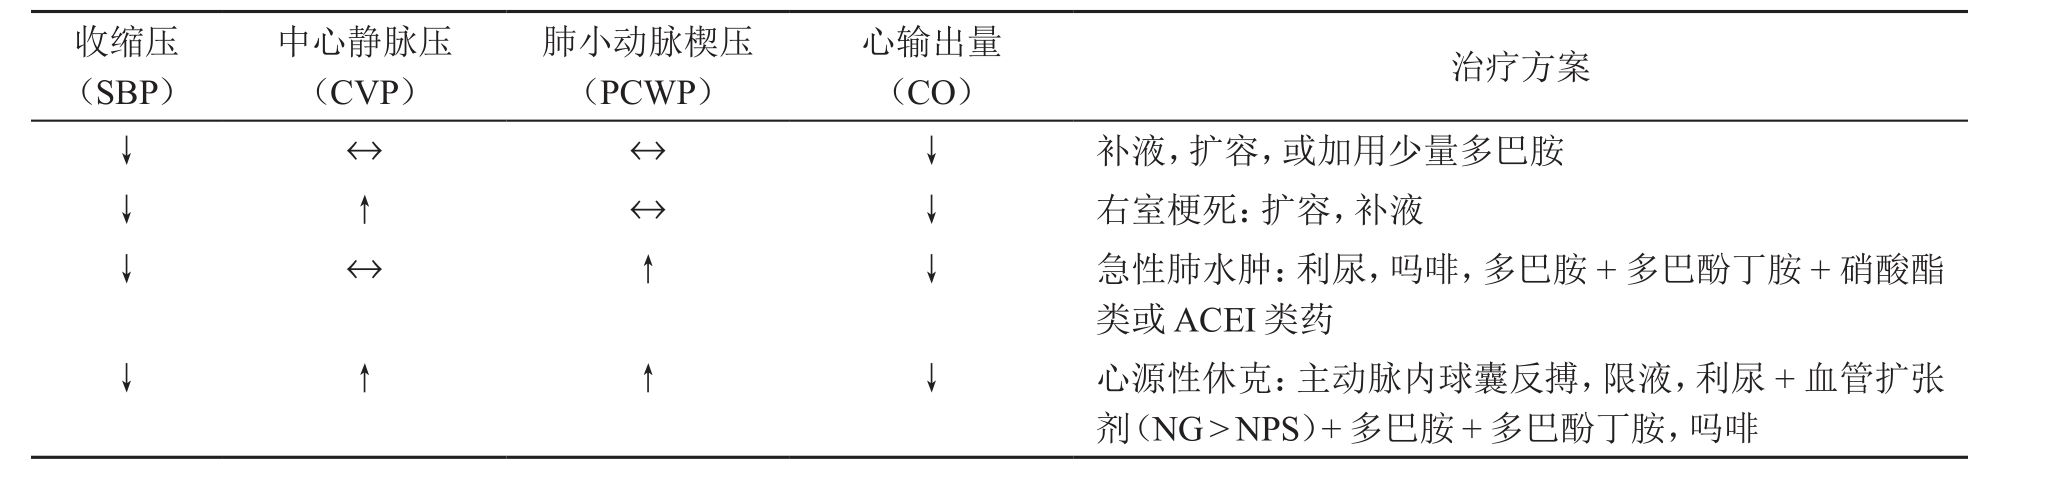
\includegraphics[width=6.8125in,height=1.65625in]{./images/Image00089.jpg}
\end{table}

\paragraph{药物}

硝酸酯类、β受体阻断剂、ACEI等药物有助于改善心肌梗死预后,但在心源性休克时可加重低血压,故以上药物在患者病情稳定前应暂停使用。为控制静脉补液量,应尽量进行微泵静脉给药。

\subsubsection{改善心脏功能及外周循环状况}

心源性休克患者存在泵衰竭及外周循环衰竭,除一般抗休克治疗外,应针对以上情况进行治疗。如患者血容量足够仍出现组织低灌注,则应予正性肌力药物加强心肌收缩力治疗及血管活性药物支持治疗。

\paragraph{正性肌力药物}

原则上应选用增加心肌收缩力而不会大幅增加心肌耗氧、维持血压而不加快心率甚至导致心律失常的药物。

\hypertarget{text00059.htmlux5cux23CHP2-3-3-2-1-1}{}
(1) 多巴酚丁胺:

为选择性β\textsubscript{1}
-肾上腺素能受体激动剂,可以在不显著增加心率及外周血管阻力的情况下增加心肌收缩力及心输出量,较少增加心肌耗氧,同时降低LVEDP,在急性心肌梗死、肺梗死等所致心源性休克患者可作为首选正性肌力药,常用剂量5~15μg/(kg•min),逐渐调整给药速度至血流动力学指标改善,但连用72小时以上会出现受体耗竭导致药效下降。

\hypertarget{text00059.htmlux5cux23CHP2-3-3-2-1-2}{}
(2) 强心苷:

有可靠的正性肌力作用,但由于心源性休克时缺血和正常心肌在交感神经兴奋及儿茶酚胺释放等影响下心电活动不稳定性增加,合并氧合不足及低钾低镁时则更不稳定,可诱发严重心律失常,而且损伤心肌对药物反应下降,对洋地黄类毒性增加,故在心源性休克时强心苷应用有所限制,仅在其他药物效果欠佳及合并快速性室上性心律失常时使用,应用时剂量减少,并应选用短效制剂如毛花苷丙等。

\hypertarget{text00059.htmlux5cux23CHP2-3-3-2-1-3}{}
(3) 磷酸二酯酶抑制剂:

通过抑制磷酸二酯酶Ⅲ的活性从而减少cAMP降解,cAMP增加活化胞膜通道令钙离子动员增加,心肌细胞内钙离子浓度增加而令其收缩功能增强,对血管特别是肺循环血管有一定的扩张作用,半衰期长,其正性时相作用及致心律失常作用较小。常用药物有氨力农及米力农,后者效果更强,应用时首先予以负荷量随后继续静脉维持,氨力农负荷量0.5~0.75mg/kg静脉注射(大于10分钟),继以5~10μg/(kg•min)静脉滴注,每日总剂量不超过10mg/kg;米力农负荷量25~50μg/kg静脉注射(大于10分钟),继以0.25~0.50μg/(kg•min)静脉滴注。此类药物不宜长期维持。常见不良反应有低血压和心律失常。

\hypertarget{text00059.htmlux5cux23CHP2-3-3-2-1-4}{}
(4) 钙离子通道增敏剂:

左西孟旦(levosimendan)是一种钙增敏剂,通过结合于心肌细胞上的肌钙蛋白C促进心肌收缩,还通过介导ATP敏感的钾通道而发挥血管舒张作用和轻度抑制磷酸二酯酶的效应。其正性肌力作用独立于β肾上腺素能刺激,可用于正接受β受体阻滞剂治疗的患者。临床研究表明,急性心衰患者应用本药静脉滴注可明显增加CO和每搏量,降低PCWP、全身血管阻力和肺血管阻力;冠心病患者不会增加病死率。用法:首剂12~24μg/kg静脉注射(大于10分钟),继以0.1μg/(kg•min)静脉滴注,可酌情减半或加倍。对于收缩压<
100mmHg的患者,不需要负荷剂量,可直接用维持剂量,以防止发生低血压。

\hypertarget{text00059.htmlux5cux23CHP2-3-3-2-1-5}{}
(5) 重组人B型利钠肽(recombinate human B-type natriuretic
peptide,rhBNP):

急性失代偿性心力衰竭患者BNP血药浓度增高,心衰越重,BNP含量越高。机体内源性分泌BNP增多是一种代偿性的自救机制,当房内压高时分泌,以拮抗醛固酮。不仅可拮抗醛固酮的水钠潴留和心脏的重构,还能均衡地扩张动、静脉,拮抗肾素-血管紧张素系统、交感神经系统、内皮素系统和血管加压素系统在心力衰竭时过度代偿带来的循环系统效率降低。代偿不足,且患者存在对BNP的抵抗。故需要外源性补充BNP。

rhBNP近几年刚应用于临床,属内源性激素物质,与人体内产生的BNP完全相同。国内制剂商品名为新活素,国外同类药名为奈西立肽(nesiritide)。其主要药理作用是扩张静脉和动脉(包括冠状动脉),从而降低前、后负荷,在无直接正性肌力作用情况下增加CO,故将其归类为血管扩张剂。实际该药并非单纯的血管扩张剂,而是一种兼具多重作用的治疗药物;可以促进钠的排泄,有一定的利尿作用;还可抑制RAAS和较高神经系统,阻滞急性心衰演变中的恶性循环。该药临床试验的结果尚不一致。晚近的两项研究(VMAC和PROACTION)表明,该药的应用可以带来临床和血流动力学的改善,推荐应用于急性失代偿心衰。国内一项Ⅱ期临床研究提示,rhBNP较硝酸甘油静脉制剂能够显著降低PCWP,缓解患者的呼吸困难。应用方法:先给予负荷剂量1.5μg/kg,静脉缓慢推注,继以0.0075~0.0150μg/(kg•min)静脉滴注;也可不用负荷剂量而直接静脉滴注。疗程一般3天,不超过7天。

\paragraph{血管活性药物}

包括拟交感神经药、血管扩张药等。

\hypertarget{text00059.htmlux5cux23CHP2-3-3-2-2-1}{}
(1) 拟交感神经药:

以多巴胺、多巴酚丁胺为主的升压药和正性肌力药物是药物支持的中心环节,但以增加心肌氧耗和能量消耗为代价而改善血流动力学,临床上应尽可能小剂量使用以维持冠状动脉和重要脏器的灌注直至IABP置入或休克缓解。大剂量的升压药已被证实降低存活率,可能与其潜在的血流动力学恶化和直接的心脏毒性作用有关。ACC/AHA推荐去甲肾上腺素用于更加严重的低血压患者(≤70mmHg)。NOS抑制剂可竞争性抑制NO的合成,目前临床上试用的甲基-L-精氨酸(L-NMMA)使CS患者平均动脉压明显升高、尿量增加,静脉注射10分钟后即可起效;使持续性CS患者30天病死率由67\%降至27\%。

多巴胺曾是心源性休克时首选的血管活性药,同时兼有正性肌力作用。小剂量{[}≤2.5μg/(kg•min){]}兴奋DA\textsubscript{1}
受体,改善肾、脑、冠脉血流,同时兴奋突触前膜上的DA\textsubscript{2}
受体,减少内源性去甲肾上腺素释放;中剂量(2.5~10μg/
kg•min)兴奋β\textsubscript{1}
受体,令肾血流增加同时又令心肌收缩力增加,心率加快心输出量增加,外周血管阻力变化不一;大剂量{[}>
10μg/(kg•min){]}兴奋外周多数血管α受体,致血管收缩,血压升高。在心源性休克时多采用中剂量,达到大剂量时仍然不能使血压升高,则可加入间羟胺一同使用,多巴胺由于会增加心率及外周血管阻力,可能会加重心肌缺血。间羟胺与去甲肾上腺素作用类似,但较之弱而持久,对α、β受体都有作用,可用于协同多巴胺升高血压。无效时和严重低血压时可用去甲肾上腺素0.5~1.0mg加入5\%葡萄糖液100ml内以2~8μg/min静脉滴注。

\hypertarget{text00059.htmlux5cux23CHP2-3-3-2-2-2}{}
(2) 血管扩张药:

单独使用血管扩张剂可使心输出量增加和左室充盈压下降,但由于冠状动脉灌注压也明显降低,血管扩张剂会导致心肌灌注进一步恶化,加重循环恶化。因此只有在各种升压措施处理后血压仍不升,而PCWP增高(PCWP
> 18mmHg),心排血量低{[}CI < 2.2L/(min•m\textsuperscript{2}
){]}或周围血管显著收缩致四肢厥冷并有发绀时使用。血管扩张剂应与正性肌力药物联合应用。硝普钠从15μg/min开始,每5分钟逐渐增加至PCWP降至15~18mmHg;硝酸甘油从10~20μg/min开始,每隔5~10分钟增加5~10μg/min,直至左室充盈压下降。对有心动过缓或房室传导阻滞的CS,可用胆碱能受体阻滞剂如山莨菪碱静滴。一般情况下血管扩张剂与正性肌力药和主动脉内气囊反搏术联合应用,能增加心输出量,维持或增加冠状动脉灌注压。

\paragraph{利尿剂}

主要用于控制肺淤血、肺水肿,同时有助于改善氧合,但可能对血压产生影响。

\subsubsection{机械循环支持}

\paragraph{主动脉内球囊反搏(intra-aortic balloon pump,IABP)}

是对CS患者机械支持治疗的主要手段,是维持血流动力学稳定的有效措施,主要通过舒张期球囊充气以改善冠状动脉和外周血流灌注,收缩期球囊放气使后负荷明显减轻从而提高左心室功能。IABP适应证:①血流动力学不稳定,患者需要循环支持以做心导管检查,冠状动脉造影以发现可能存在的外科手术可纠正的病变,或是为冠状动脉旁路移植术(GABG)或经皮冠状动脉介入治疗(PCI);②对内科治疗无效的;③患者有持续性心肌缺血性疼痛,对100\%氧吸入、β受体阻滞剂和硝酸酯治疗无效的患者。SHOCK登记研究显示接受IABP的患者病死率明显下降,尤其是对于接受溶栓治疗的患者。因此,只要条件允许,应尽快在血运重建前置入IABP。ACC/AHA和ESC指南均将置入IABP列为药物治疗无效CS的Ⅰ类适应证。但并非所有患者均对IABP有血流动力学反应,也并非所有患者均能从IABP中获益,如高度狭窄的冠状动脉并未显示血流灌注增加。但有反应者提示预后良好。既往IABP并发症高达10\%~30\%,现已明显降低,尤其是在IABP置入量高的中心。大样本人群研究显示,总并发症和严重并发症的发生率为7.2\%和2.8\%。主要包括肢端缺血、主动脉夹层、股动脉破裂、感染、溶血、血栓形成及栓塞等。出现该并发症的主要危险因素为女性、身材小和外周血管疾病;禁忌证包括主动脉瓣反流、主动脉夹层和外周血管疾病。

\paragraph{左心室辅助设备}

(left ventricular assist device,LVAD)
LVAD借助外置的机械设备,暂时的、部分的代替心脏的功能,有助于组织的灌注,等待心功能的恢复,并打断心源性休克时的恶性循环,是心源性休克的重要治疗措施。左心室辅助设备以外科手术方法或导管方法从机体取血。常用的取血部位为左心室和左心房,将血以一定的压力回到升主动脉。左心室辅助设备常可作为心脏移植的过渡,对何种患者需果断使用左心室辅助设备尚需进一步研究。传统的左室辅助装置的安置需体外循环下手术经胸植入,近年来经皮左室辅助装置开始(percutaneous
left ventricular assist
device,PLVAD)逐渐应用于临床。目前临床运用比较成熟的PLVAD有两种,一种经股静脉、股动脉途径建立左房股动脉引流途径,另一种经股动脉植入微型轴流泵,直接建立左室-升主动脉引流途径。研究随机比较了PLVAD和IABP在急性心梗并发心源性休克中的疗效,PLVAD治疗组初级终点心脏指数及肾功能明显改善,血清乳酸水平降低,改善左室功能,但30天死亡率无明显差别。基础研究结果显示LVAD应用后可逆转心肌重构过程,并可改善心肌细胞β肾上腺素能受体信号功能,这些基础研究的发现均提示LVAD可能改善心衰及心源性休克患者的预后。

\subsubsection{血流重建治疗}

心源性休克最主要的病因是急性心肌梗死,重建冠脉血流对于恢复心肌供血及心肌功能有关键性的意义。

\paragraph{溶栓治疗}

对于急性心肌梗死,溶栓治疗已经被确认有助于降低急性心肌梗死的病死率,然而溶栓治疗在心源性休克中的地位尚未完全明确,早期溶栓治疗有助于降低心源性休克的发生率,但对于已经发生心源性休克的患者,多个临床试验未能证明溶栓治疗可以降低病死率。这个结果与患者的冠脉再灌注率有关,多数心源性休克患者冠脉再灌注失败,而在少数再灌注成功的患者,可以观察到病死率的下降。目前认为,血流动力学、机械因素以及代谢因素影响了溶栓治疗在心源性休克患者治疗中的作用,当心源性休克时由于动脉压力下降,溶栓药物较少到达栓子,梗死灶内血管在低血压时发生塌陷也影响了溶栓药物的作用,酸中毒则影响了纤维蛋白酶原向纤维蛋白原的转化。部分临床试验支持同时采用血管活性药物可以改善溶栓效果。

\paragraph{血管重建}

包括直接血管重建以及冠状动脉旁路手术。直接血管重建,包括经皮穿刺冠状动脉成形术(PTCA)及支架植入等,PTCA可以令80\%~90\%急性心肌梗死患者的狭窄血管达到TIMI
3级的血管通畅度,高于溶栓治疗的成功率(50\%~60\%),部分临床试验更指出,在高危患者(年龄>
70岁,大面积心肌梗死,心率>
100次/分)PTCA较溶栓治疗能更多地减低病死率。因此,对心源性休克患者进行急诊直接血管重建可能有益,除了改善梗死灶处心肌活动,梗死灶远端的心肌收缩力也有改善。而在进行PTCA同时植入支架,又能改善不能成功完成PTCA患者的存活率。血管重建后的抗血小板治疗对维持冠脉通畅有意义,血小板糖蛋白Ⅱb/Ⅲa受体拮抗剂应用可以改善近期内血管重建术的预后。冠状动脉旁路手术(CABG)同样被多项临床试验支持对心源性休克患者有益,然而手术进行需时而且手术有较高的机会出现各种并发症,令CABG应用受到限制。

\subsubsection{特殊情况的心源性休克治疗}

\paragraph{右室心肌梗死}

约30\%的下壁心肌梗死患者合并右室心肌梗死,患者表现为低血压、颈静脉充盈怒张、肺野清晰,右胸导联的心电图检查可发现典型的ST-T改变,右心内导管检查可发现RAP及RVEDP升高及PCWP正常或下降,CO下降,超声心动图提示右室心肌收缩力下降。右室心肌梗死患者发生心源性休克其预后稍好。通过补液维持右室前负荷,然而补液可能在增高PCWP后而不能令CO增加,右室过度充盈会导致心肌耗氧增加,降低右冠状动脉的灌注压,加重右心心肌缺血,也会影响左心室的充盈及CO。多巴酚丁胺治疗可有助于改善CO。血流动力学持续不稳定的患者采用IABP可能有益。恢复右心冠脉血流对改善预后有重要作用。

\paragraph{急性二尖瓣反流}

下壁心肌梗死、乳头肌缺血或梗死都可能导致急性二尖瓣反流,多发生于心肌梗死后2~7天,发生急性二尖瓣反流时会在短时间内出现肺水肿、低血压及心源性休克,当乳头肌断裂时心脏杂音仅在收缩早期可闻而且往往柔和甚至听不到,主要是因为左房左室内的压力差迅速消失。超声心动图可以迅速诊断,血流动力学监测有一定帮助,治疗上可用硝普钠降低后负荷,IABP有助于暂时控制病情,正性肌力药及血管活性药有助于维持CO及血压,手术修补或更换受损瓣膜是唯一彻底的治疗方法并且应尽早进行。

\paragraph{室间隔破裂}

患者表现为严重心功能衰竭及心源性休克,可闻及全收缩期杂音及触及心前区震颤,血流动力学监测发现左向右分流表现(右室内血氧饱和度升高),超声心动图有助于确诊。早期行IABP及药物支持,争取尽快进行手术治疗,一般建议是在发生破裂后的48小时内。

\paragraph{室壁破裂}

多发生于急性心肌梗死后第1周内,常见于老年女性伴高血压患者,早期溶栓治疗可以降低发生率。患者表现为急性心包填塞,应尽早认识到病情并行紧急心包穿刺抽液,减轻心包填塞,尽早行手术治疗。

\protect\hypertarget{text00060.html}{}{}

\hypertarget{text00060.htmlux5cux23CHP2-3-4}{}
参 考 文 献

1. Reynolds HR,Hochman JS. Cardiogenic shock:current concepts and
improving outcomes. Circulation,2008,117:86-697

2. 刘品明
.急性心肌梗死伴心源性休克.中华心血管病杂志,2009,37(10):956-960

3. Trost JC,Hillis LD. Intra-aortic balloon counterpulsation. Am J
Cardiol,2006,97(9):1391-1398

4. Buja LM. Myocardial ischemia and reperfusion injury. Cardiovasc
Pathol,2005,14(4):170-175

5. Bedi MS,Alvarez RJ,Jr.,Kubota T,et al. Myocardial Fas and
cytokine expression in end-stage heart failure:impact of LVAD support.
Clin Transl Sci,2008,1(3):245-248

\protect\hypertarget{text00061.html}{}{}

\chapter{失血性休克}

失血性休克(hemorrhagic
shock)是各种创伤和疾病引起的急性失血所导致循环血容量短期内丢失超过机体应急代偿能力而出现的有效循环血量与心排血量减少,继而引起组织灌注不足、细胞代谢紊乱和功能受损的一系列病理生理过程。是休克最常见的一种类型,系最具有代表性的低血容量性休克(hypovolemic
shock)。失血性休克的主要病理生理改变是有效循环血容量急剧减少,导致组织低灌注、无氧代谢增加、乳酸性酸中毒、再灌注损伤以及内毒素易位,最终导致的多器官功能障碍综合征(MODS)。其主要死因是组织低灌注以及大出血、感染和再灌注损伤等原因导致的MODS。

\subsection{病因与发病机制}

失血性休克的常见病因有:严重创伤、骨折、挤压伤等所致的外出血和内脏(如肝脾)破裂引起内出血;各种原因如消化性溃疡、急性胃黏膜病变、食管胃底静脉曲张破裂等所致的消化道出血;呼吸道出血引起的咯血;泌尿道出血引起的血尿;女性生殖道出血引起的阴道流血;腹腔、腹膜后、纵隔等出血、动脉瘤破裂出血等内出血。其中,创伤是急性失血性休克的最常见原因。

上述各种原因所致的内出血或外出血,都造成有效循环血容量丧失。有效循环血容量丢失触发机体各系统器官产生一系列病理生理反应,以保存体液,维持灌注压,保证心、脑等重要器官的血液灌流。

低血容量导致交感神经-肾上腺轴兴奋,儿茶酚胺类激素释放增加并选择性地收缩皮肤、肌肉及内脏血管。其中动脉系统收缩使外周血管总阻力升高以提升血压;毛细血管前括约肌收缩导致毛细血管内静水压降低,从而促进组织间液回流;静脉系统收缩使血液驱向中心循环,增加回心血量。儿茶酚胺类激素使心肌收缩力加强,心率增快,心排血量增加。

低血容量兴奋肾素-血管紧张素Ⅱ-醛固酮系统,使醛固酮分泌增加,同时刺激压力感受器促使垂体后叶分泌抗利尿激素,从而加强肾小管对钠和水的重吸收,减少尿液,保存体液。

上述代偿反应在维持循环系统功能相对稳定,保证心、脑等重要生命器官的血液灌注的同时,也具有潜在的风险。这些潜在的风险是指代偿机制使血压下降在休克病程中表现相对迟钝和不敏感,导致若以血压下降作为判定休克的标准,必然贻误对休克时组织灌注状态不良的早期认识和救治;同时,代偿机制对心、脑血供的保护是以牺牲其他脏器血供为代价的,持续的肾脏缺血可以导致急性肾功能损害,胃肠道黏膜缺血可以诱发细菌、毒素易位。内毒素血症与缺血-再灌注损伤可以诱发大量炎性介质释放入血,促使休克向不可逆发展。

机体对低血容量休克的反应还涉及代谢、免疫、凝血等系统,同样也存在对后续病程的不利影响。肾上腺皮质激素和前列腺素分泌增加与泌乳素分泌减少可以造成免疫功能抑制,患者易于受到感染侵袭。缺血缺氧、再灌注损伤等病理过程导致凝血功能紊乱并有可能发展为弥漫性血管内凝血。

组织细胞缺氧是休克的本质。休克时微循环严重障碍,组织低灌注和细胞缺氧,糖的有氧氧化受阻,无氧酵解增强,三磷酸腺苷(ATP)生成显著减少,乳酸生成显著增多并组织蓄积,导致乳酸性酸中毒,进而造成组织细胞和重要生命器官发生不可逆性损伤,直至发生MODS。

\subsection{诊断}

\subsubsection{临床表现特点}

对于因胃肠道、呼吸道、泌尿道、生殖道等发生大量出血所致的休克,由于出血一般均排出体外,诊断较易;但消化道出血有时在出现呕血和便血之前即有休克,如未注意,可延误诊断。

腹腔内出血常见者为脾破裂、异位妊娠破裂出血。脾破裂患者常有腹部外伤史,但有时可自发破裂,此时脾脏常因有充血或感染而肿大,故易于破裂,患者常先有左上腹疼痛,以后转为全腹部,且伴有腹部压痛和移动性浊音,诊断性腹腔穿刺可以确诊。异位妊娠破裂出血的患者常有短期(一般6~7周)闭经史,继而有阴道流血和腹痛。腹痛剧烈,首先位于下腹部,且有腹部移动性浊音。妇科检查有少量阴道出血,宫口闭,宫体可扩大,但不及应有孕期的大小。宫体的一侧可有清楚块质,且有压痛,阴道后穹隆膨出,经后穹隆穿刺可得血液而确诊。

胸腔出血可由外伤、肿瘤、胸膜粘连带的撕裂以及主动脉夹层等引起。患者常先有一侧胸痛,随呼吸而加剧,叩诊变浊,呼吸音降低。出血如在500ml以上,胸部X线可发现胸腔积液。确诊在于胸腔穿刺抽到血液。

因骨折而出血有时亦可引起休克,尤其是骨盆、股骨等骨折,出血迅速而量大,可在1000ml以上而外观可不明显,休克较易发生。例如:脊柱、盆腔骨折可因腰部静脉撕破而致腹膜后大量出血,血液能积存于组织间隙高达2000ml以上;股骨骨折时血液可储存于大腿的软组织中,虽积血达1000~1500ml也常不发生令人注目的急性肿胀。诊断时应特别重视。

此外,流行性出血热、肝破裂、肾破裂、腹主动脉瘤破裂、肿瘤(如肝癌结节破裂)、各种出血性疾病、应用抗凝剂等也可引起腹腔内或腹膜后大出血而发生休克,应予以足够的警惕。

失血量的临床估计方法可参考表\ref{tab22-1}。

\begin{table}[htbp]
\centering
\caption{失血量的临床估计方法}
\label{tab22-1}
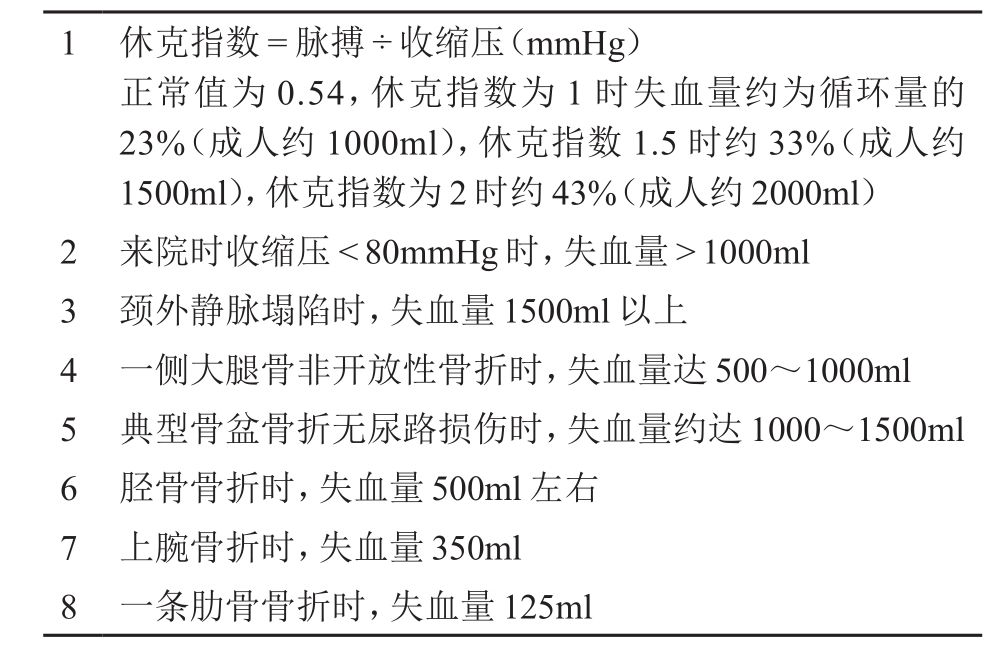
\includegraphics[width=3.33333in,height=2.17708in]{./images/Image00090.jpg}
\end{table}

不论失血的病因如何,失血性休克多表现为冷型休克(低排高阻型休克),突出的表现特点是“5P”:皮肤苍白(pallor)、冷汗(prespiration)、虚脱(prostration)、脉搏细弱(pulselessness)、呼吸困难(pulmonary
dificiency)。最初反应为交感神经兴奋,表现为精神紧张、烦躁、皮肤苍白、出冷汗、四肢末端发凉、脉细速,血压可正常但脉压小;若出血量大或在较晚期血压常下降,并有呼吸困难。

\subsubsection{诊断注意事项}

失血性休克的早期诊断对预后至关重要。传统的诊断主要依据为病史、症状、体征,包括精神状态改变、皮肤湿冷、收缩压下降(<
90mmHg或较基础血压下降> 40mmHg)或脉压减少(< 20mmHg)、尿量<
0.5ml/(kg•h)、心率>100次/分、中心静脉压(CVP)<
5mmHg或肺动脉楔压(PAWP)<
8mmHg等指标。对于多发创伤和以躯干损伤为主的失血性休克患者,床边超声可以早期明确出血部位从而早期提示手术的指征;CT检查比床边超声有更好的特异性和敏感性。氧代谢与组织灌注指标对失血性休克早期诊断有更重要参考价值。

\subsubsection{失血性休克的分级}

临床上,根据失血量等指标可将失血性休克分成四级(以体重70kg的成年男性为例):

Ⅰ级(早期):失血量< 750ml,占血容量比例<
15\%,心率(HR)≤100次/分,血压正常或稍增高;

Ⅱ级(代偿期):失血量750~1500ml,占血容量比例15\%~30\%,HR >
100次/分,呼吸增快(20~30次/分),血压下降,皮肤苍白、发凉,毛细血管充盈延迟,轻~中度焦虑,尿量减少(20~30ml/h);

Ⅲ级(进展期):失血量1500~2000ml,占血容量比例30\%~40\%,HR >
120次/分,呼吸急促(30~40次/分),血压明显下降,神志改变如萎靡或躁动不安,尿量明显减少(5~20ml/h);

Ⅳ级(难治期):失血量> 2000ml,占血容量比例> 40\%,HR >
140次/分,脉搏细弱,呼吸窘迫(>
40次/分),血压显著下降,皮肤发绀、湿冷,意识障碍,无尿。

大量失血定义为24小时内失血超过患者的估计血容量或3小时内失血量超过估计血容量的一半。

\subsubsection{失血性休克的监测}

\paragraph{一般临床监测}

包括皮温与色泽、心率、血压、尿量和精神状态等监测指标。尿量是反映肾灌注较好的指标,可以间接反映循环状态。当尿量<
0.5ml/(kg•h)时,应继续进行液体复苏。需注意临床上患者出现休克而无少尿的情况,如高血糖和造影剂等有渗透活性的物质造成的渗透性利尿。血压的变化需要严密地动态监测。休克初期由于代偿性血管收缩,血压可能保持或接近正常。对未控制出血的失血性休克维持“允许性低血压”(permissive
hypotention),即维持平均动脉压(MAP)在60~80mmHg。

\paragraph{有创血流动力学监测}

包括:①MAP监测:有创动脉血压(IBP)较无创动脉血压(NIBP)高5~20mmHg。持续低血压状态时,NIBP测压难以准确反映实际大动脉压力,而IBP测压较为可靠,可保证连续观察血压和即时变化。②CVP和PAWP监测:CVP和PAWP监测有助于对已知或怀疑存在心功能不全的休克患者的液体治疗,防止输液过多导致的前负荷过度。③心排量(CO)和每搏量(SV)监测:连续监测CO与SV,有助于动态判断容量复苏的临床效果与心功能状态。

\paragraph{氧代谢监测}

传统临床监测指标往往不能对组织氧合的改变具有敏感反应,此外,经过治疗干预后的心率、血压等临床指标的变化也可在组织灌注与氧合未改善前趋于稳定。因此,同时监测和评估一些全身灌注指标如氧输送(oxygen
delivery,DO\textsubscript{2} )、氧消耗(oxygen
consumption,VO\textsubscript{2}
)、血乳酸、混合静脉血氧饱和度(saturation of mixed venous blood
oxygen,SvO\textsubscript{2} )或中心静脉血氧饱和度(saturation of
central venous blood oxygen,ScvO\textsubscript{2}
)等以及局部组织灌注指标如胃黏膜内pH(pHi)与胃黏膜CO\textsubscript{2}
张力(PaCO\textsubscript{2} of gastric mucosa,PgCO\textsubscript{2}
)等具有较大的临床意义。其中,动脉血乳酸浓度是反映组织缺氧的高度敏感的指标之一,动脉血乳酸增高常较其他休克征象先出现。持续动态的动脉血乳酸以及乳酸清除率监测对休克的早期诊断、判定组织缺氧情况、指导液体复苏及预后评估具有重要意义。碱缺失(base
deficit,BD)可间接反映血乳酸的水平。当休克导致组织供血不足时碱缺失下降,提示乳酸血症的存在。碱缺失可分为:轻度(−2~−5mmol/L),中度(<
−5~≥−15mmol/L),重度(<
−15mmol/L)。碱缺失与血乳酸结合是判断休克组织灌注较好的方法。

\paragraph{实验室监测}

包括:①血常规监测:动态观察红细胞计数、血红蛋白(Hb)及血细胞比容(Hct)的数值变化,对失血性休克的诊断和判断是否存在继续失血有参考价值。②电解质监测与肾功能监测:对了解病情变化和指导治疗十分重要。③凝血功能监测:常规凝血功能监测包括血小板计数、凝血酶原时间(PT)、活化部分凝血活酶时间(APTT)、国际标准化比值(international
normalized
ratio,INR)和D-二聚体等。若PT和(或)APTT延长至正常值的1.5倍,即应考虑凝血功能障碍。

\subsection{治疗}

包括原发病治疗(止血)和纠正休克(补充血容量)两个方面。原发病的有效治疗是失血性休克抢救成功的基础。创伤后引起大出血,尤其是难以控制的大出血,多在伤后1~2小时内死亡,因此伤后的“黄金1小时”内应以挽救生命为主。而“黄金1小时”的前10分钟尤为重要,多因血容量急剧减少而诱发心脏骤停,被称为“白金10分钟”。因此,对于急性失血性休克的最初阶段,应以适当扩充血容量以避免心脏骤停为主要目标;同时处理失血原因及相关并发症是赢取救治时间的关键。

\subsubsection{原发病治疗(止血)}

原发病的有效治疗是失血性休克抢救成功的基础。对于出血部位明确、存在活动性出血的休克患者,应尽快进行手术或介入止血。不去设法制止出血,只顾用输血来补充血量以纠正休克状态,是无效和错误的,治疗出血的首要任务是止血。在补充血容量的同时,应尽快进行止血,否则,在不断出血的情况下,尽管积极补液、输血,血容量仍不会恢复,休克也不会得到纠正。原则上是先采用暂时止血措施,待休克初步纠正后,再进行根本的止血措施;但是在难以用暂时止血的措施止血时,即应一面补充血容量,一面施行根本的止血措施。

采用何种止血方法,应根据出血来源而定:①四肢、头颅或身体表浅部位的较大出血,可先采用填塞、加压包扎暂时止血,待休克基本纠正后,再作手术处理。②内脏脏器如肝、脾破裂、宫外孕破裂等出血,则应尽早进行手术。③各种原因的上消化道出血、咯血,一般宜行内科保守治疗,必要时可考虑手术。

\subsubsection{补充血容量(液体复苏)}

液体复苏的目的是维持机体血流动力学的稳定,纠正代谢紊乱,恢复组织器官的正常灌注。

\hypertarget{text00061.htmlux5cux23CHP2-4-3-2-1}{}
(一) 液体复苏的发展

\paragraph{立即液体复苏}

经典的失血性休克液体复苏方法始于20世纪60年代,并被美国外科医师学院规范在创伤生命支持高级训练课程(ATLS)中,其主要内容是:一旦确认发生失血性休克,便立即和迅速地给予大容量输液,要求维持血压在正常范围内,直至出血被制止,这个过程被描述为“stay
and treat”(停下来抢救)。

\paragraph{延迟液体复苏}

近十多年的研究结果对上述经典的失血性休克液体复苏方法提出强力挑战。Bickell与Turner等的研究结果显示“早期不进行液体复苏比进行液体复苏的预后要好”。这种与经典的失血性休克液体复苏方法预料相悖的结果,其原因除了早期复苏可能延误决定性治疗(如外科手术)外,最主要原因是,在出血未被有效控制的情况下,大容量液体复苏和提升血压可以导致持续出血、血液稀释和体温下降,进而造成氧输送不足、凝血功能障碍和低体温,构成所谓“死亡三角”。对此,一些学者提出,在出血未被有效制止前,应该尽快将伤员转送到有手术条件的医院,复苏只在即将手术前才开始进行,这个策略被称作“scoop
and run”(卷起就跑)。

\paragraph{限制性液体复苏}

多数学者研究认为,对失血性休克是否需要早期复苏取决于失血的情况和伤员状态,为避免伤员在短期内死亡,对大出血和严重休克患者给予液体复苏是必要的,但同时也应该避免因快速和大量液体复苏所引发的问题。这样,提出了一个主张低度干预的复苏策略------“treat
and
run”(边治边走):要求用尽可能少的液体将血压维持在能够勉强保持组织灌注的较低水平,即“可允许性低血压”(permissive
hypotension)(收缩压80~90mmHg或MAP
60~80mmHg)。这种输液量因患者而宜,有活动性出血的休克患者,出血未控制之前不主张早期快速给予大量的液体进行复苏,在到达手术室彻底止血前,给予一定量的液体维持机体的基本需要,在相应的手术处理后再进行常规液体复苏,此即限制性液体复苏。研究证实:限制性液体复苏策略可降低病死率、减少再出血率及并发症。

限制性液体复苏策略已经开始向临床推荐。2003年美国和加拿大创伤学会提出了战场条件下休克的液体复苏方案:①评估是否需要复苏主要依据伤员的意识和脉搏状态;②如伤员意识清楚、桡动脉有力,不需给予任何输液;③对脉搏微弱和意识水平降低者应给予输液;④复苏应使收缩压维持在80~85mmHg;⑤复苏应给予小剂量的高渗晶体或人工胶体液。

但早期限制性液体复苏是否适合各类失血性休克,需维持多高的血压,可持续多长时间尚未有明确的结论。对于颅脑损伤患者,合适的灌注压是保证中枢神经组织氧供的关键。颅脑损伤后颅内压增高,此时若机体血压降低,则会因脑血流灌注不足而继发脑组织缺血性损害,进一步加重颅脑损伤。因此,一般认为对于合并颅脑损伤的严重失血性休克患者,宜早期输液以维持血压,必要时合用血管活性药物,将收缩压维持在正常水平,以保证脑灌注压,而不宜延迟复苏。允许性低血压在老年患者应谨慎使用,在有高血压病史的患者也应视为禁忌。

\hypertarget{text00061.htmlux5cux23CHP2-4-3-2-2}{}
(二) 液体复苏常用的液体种类

\paragraph{晶体溶液}

常用有生理盐水、复方氯化钠注射液(林格液)、乳酸钠林格注射液(平衡盐溶液,简称平衡液)、高渗盐溶液等。生理盐水含钠、氯浓度均为154mmol/L,电解质浓度308mmol/L;复方氯化钠注射液含钠、钾、钙、氯浓度分别为146mmol/L、4mmol/L、2.5mmol/L、155mmol/L,电解质浓度307.5mmol/L;乳酸钠林格注射液含钠、钾、钙、氯浓度分别为130mmol/L、4mmol/L、1.5mmol/L、109mmol/L,电解质浓度272.5mmol/L。乳酸钠林格注射液是液体治疗或复苏时最常用的晶体液。高渗盐溶液有7.5\%氯化钠注射液和3\%氯化钠注射液。高渗晶胶溶液有7.5\%氯化钠注射液+
6\%右旋糖酐溶液(HSD)和4.2\%氯化钠注射液+羟乙基淀粉(霍姆)等制剂。

失血性休克时有明显的细胞外液减少和细胞内液增加。生理盐水、复方氯化钠注射液、乳酸钠林格注射液主要分布于细胞外液,输注的晶体液约有25\%存留在血管内,而其余75\%则分布于血管外间隙。临床上输注1L等张晶体液后,血管内容量可增加100~200ml。复方氯化钠注射液中所含的乳酸在复苏过程中可以迅速代谢,不会影响动脉血乳酸测定。等渗电解质液无携氧功能,改善血流动力学效果差和时间短,用其单独纠正严重休克时其用量需为失液量的3~4倍才能维持循环,而且往往在输液结束后即有70\%~80\%漏到了血管外,大量输入等渗液有可能会进一步增加细胞与组织的水肿。

高渗盐溶液治疗机制是高渗和提高循环渗透压作用使细胞与组织脱水,细胞内和组织中的水分至血管中起到自体输液的作用,达到扩张有效循环血量的作用,使组织灌注好转及尿量增加,使血流动力学及全身情况获得明显改善。7.5\%氯化钠注射液4ml/kg输入休克机体后,扩充血浆容量约8ml/kg,等量的高渗晶胶溶液增加的血浆容量约14ml/kg,增加的血浆容量维持时间可达2小时。与等渗电解质液相比,其好处是用量小,能产生明显的血流动力学效果和改善组织水肿。对存在颅脑损伤的患者,由于可以很快升高MAP而不加剧脑水肿,因此高渗盐溶液可能有很好的前景。

休克患者应不给含糖液体,尤其是伴有中枢神经系统损伤的患者应禁止补充含糖液体,尽管补充含糖液体也可提升血压,但输注含糖液体后可引起和加重再灌注损伤。

\paragraph{胶体溶液}

临床上可供使用的有:

\hypertarget{text00061.htmlux5cux23CHP2-4-3-2-2-2-1}{}
(1) 右旋糖酐:

包括右旋糖酐40(低分子右旋糖酐)和右旋糖酐70(中分子右旋糖酐)。前者扩容效果较差,且持续时间短暂,有渗透性利尿作用,静脉滴注每次250~500ml,每日不超过20ml/kg;后者扩容效果与血浆相似,每克可结合水25ml左右,扩容效果可维持12小时,静脉滴注每次500ml,每日最大量不超过1000~1500ml。

\hypertarget{text00061.htmlux5cux23CHP2-4-3-2-2-2-2}{}
(2) 琥珀酰明胶(血定安,佳乐施):

为胶体性代血浆,扩容效能类似于4\%白蛋白。可增加血浆容量,使静脉回流及心输出量增加,改善微循环,增加血液的运氧能力;也能减轻组织水肿,有利于组织对氧的利用。其渗透性利尿作用有助于维持休克患者的肾功能。静脉输入的剂量和速度取决于患者的实际情况,严重急性失血时可在5~10分钟内输入500ml,直至低血容量症状缓解。大量输入时应确保维持Hct不低于0.25。

\hypertarget{text00061.htmlux5cux23CHP2-4-3-2-2-2-3}{}
(3) 羟乙基淀粉(淀粉代血浆,706代血浆):

输注1L能使循环容量增加700~800ml,至24小时后仍可维持40\%的最大扩容效果。静脉滴注500~1000ml。

\hypertarget{text00061.htmlux5cux23CHP2-4-3-2-2-2-4}{}
(4) 中分子羟乙基淀粉200/0.5(贺斯,haesteril):

为血容量扩充药。本品较低分子羟乙基淀粉有较高的分子量、独特的取代程度(克分子取代级MS
= 0.5)和取代方式(以C\textsubscript{2} 位置为主,C\textsubscript{2}
/C\textsubscript{6} =
5∶1),故有较强的容量扩充效应和较长的维持时间。用于预防和治疗各种原因引起的血容量不足和休克,如手术、创伤、感染、烧伤等。还有防止和堵塞毛细血管漏的作用,在毛细血管通透性增加的情况下使用本品,可减少白蛋白渗漏,减轻组织水肿,减少炎症介质产生,对危重患者更有利。有两种制剂,6\%中分子羟乙基淀粉200/0.5最大日剂量为33ml/kg,每小时最大滴速为20ml/kg;10\%中分子羟乙基淀粉200/0.5最大日剂量为20ml/kg,每小时最大滴速为20ml/kg。

\hypertarget{text00061.htmlux5cux23CHP2-4-3-2-2-2-5}{}
(5) 中分子羟乙基淀粉130/0.4(万汶,Voluven):

作用与中分子羟乙基淀粉200/0.5相似,但本品在此基础上作了进一步改良处理:适当减少分子量;降低取代级,下降约20\%(MS
= 0.4);改变了取代方式(C\textsubscript{2} /C\textsubscript{6} =
9∶1);分子量分布更加集中(减少了对血液流变学和凝血有不利影响的大分子比例,也减少了分子量低于肾阈值而快速排出小分子的比例)。这些改进使其安全性、耐受性、提高胶体渗透压的作用均有所增加。最大日剂量可用至33~50ml/kg。据患者需要可持续使用数日。中分子羟乙基淀粉130/0.4(万汶)是人血白蛋白最好的替代物,也是目前所有人工胶体溶液中最安全的药物。

\hypertarget{text00061.htmlux5cux23CHP2-4-3-2-2-2-6}{}
(6) 聚明胶肽(血代,海脉素):

扩容效能类似于琥珀酰明胶。一般500ml约在1小时内输入,急救时可在5~15分钟内输入500ml。一日最大剂量为2000ml。因钙离子浓度高达6.2mmol/L,对高钙血症、正在使用洋地黄治疗的患者禁用。

\hypertarget{text00061.htmlux5cux23CHP2-4-3-2-2-2-7}{}
(7) 白蛋白:

白蛋白是一种天然的血浆蛋白质,在正常人构成了血浆胶体渗透压的75\%~80\%。正常血浓度为35~50g/L。规格有5\%、10\%、15\%、20\%的注射液和5g、10g的冻干粉。5\%人血白蛋白溶液250ml的胶体渗透压为18~20mmHg/L,而25\%人血白蛋白溶液50ml的胶体渗透压为100mmHg/L。在复苏治疗初期,输注5\%人血白蛋白溶液1L血浆溶液增加500~1000ml。输注25\%人血白蛋白溶液100ml,如果体液能够从组织间隙进入血管内,1小时后可使血管内容量增加400~500ml。

白蛋白、新鲜或冻干血浆是液体复苏治疗时常用的胶体溶液,但其价格较昂贵,具有传播多种血道传染病的潜在危险,输入白蛋白后会发生毛细血管渗漏,将弥散至组织间质中,且不能自由地回至血管内,导致组织间质渗透压升高,组织水肿。

\hypertarget{text00061.htmlux5cux23CHP2-4-3-2-2-2-8}{}
(8) 高渗羟乙基淀粉200/0.5氯化钠注射液(贺苏):

本品为高渗胶体溶液,含7.2\%氯化钠与6\%羟乙基淀粉。由于本品的高渗作用(2464mOsm/L),液体可快速由组织间隙向血管内转移,血流动力学指标如血压、心输出量快速上升,并与输注量及输注速度有关。规格:250ml/袋。本品仅用于单次快速静脉输注或加压输注(推荐在2~5分钟内输完),用量约为4ml/kg体重(相当于体重60~70kg的患者使用250ml)。输注本品后,扩容维持时间较短,必须立即给予足够的液体治疗,以稳定血流动力学。

\hypertarget{text00061.htmlux5cux23CHP2-4-3-2-3}{}
(三) 复苏液体的选择

目前尚无足够的证据表明晶体液与胶体溶液用于低血容量休克液体复苏的疗效与安全性方面有明显差异。合理的液体选择方式是:晶体液为开始复苏的首选及主要选择(Ⅱ类证据);胶体溶液可在对晶体液复苏反应满意时加用(Ⅲ类证据);从经济方面考虑,应优先使用非蛋白类胶体溶液(Ⅱ类证据)。液体复苏时晶体液与胶体溶液比例通常为3∶1。无论用晶体液或胶体溶液,也无论用量多少,必须维持Hct在0.25以上。

\subsubsection{输血与防治凝血功能障碍}

失血性休克时,在输注晶体液和代血浆的同时,常应用新鲜冰冻血浆(FFP)、冷沉淀、浓缩血小板悬液,以改善凝血功能。

\paragraph{浓缩红细胞}

当Hb降至70g/L时应考虑输血。对于有活动性出血的患者,老年人以及有心肌梗死风险者,Hb保持在较高水平更为合理。无活动性出血的患者每输注1单位(200ml全血)的红细胞其Hb升高约10g/L,Hct升高约3\%。24小时内输血>
10单位为大量输血。但大量输注红细胞时易导致凝血紊乱,应及时补充血小板和凝血因子等特殊成分。Holcomb等报道以1∶1∶1的比例输注血浆、血小板、红细胞对预后有利。与成分输血相比,新鲜全血含有更多的凝血因子、血小板、红细胞,能更有效地纠正贫血和改善凝血功能。

\paragraph{血小板}

血小板输注主要适用于血小板数量减少或功能异常伴有出血倾向的患者。急性失血患者的血小板应维持在50
× 10\textsuperscript{9}
/L以上;严重创伤和中枢神经系统损伤的患者,应在100 ×
10\textsuperscript{9}
/L以上。对大量输血后并发凝血异常的患者联合输注血小板和冷沉淀可显著改善止血效果。

\paragraph{新鲜冰冻血浆(FFP)}

输注FFP的目的是为了补充凝血因子的不足。FFP不仅可以迅速改善凝血功能,还可起到扩容,改善微循环的作用。PT或APTT大于正常值的1.5倍时,应输入FFP纠正凝血紊乱,FFP输入量10~15ml/kg。

\paragraph{冷沉淀}

内含凝血因子Ⅴ、Ⅷ、Ⅻ、纤维蛋白原等,适用于特定凝血因子缺乏所引起的疾病、肝移植围术期以及肝硬化食管静脉曲张等出血。还可用于预防大量输血后的出血倾向。要求凝血因子活性至少在正常值的20\%~30\%,<
20\%易发生出血。

\subsubsection{血管活性药与正性肌力药}

临床通常仅对于足够的液体复苏后仍存在低血压或者输液还未开始的严重低血压患者.才考虑应用血管活性药与正性肌力药。可选用多巴胺、间羟胺、多巴酚丁胺等。

\subsubsection{纠正代谢性酸中毒}

代谢性酸中毒的处理应着眼于病因处理、容量复苏等干预治疗,在组织灌注恢复过程中酸中毒状态可逐步纠正,过度的血液碱化使氧解离曲线左移,不利于组织供氧。因此,在失血性休克的治疗中,碳酸氢盐的治疗只用于紧急情况或pH
< 7.20时,不主张常规使用。

\subsubsection{早期恰当使用止血药物}

严重出血无疑会导致凝血功能的异常,这就为抗纤溶药物的使用提供了可能。最近一项高质量的临床试验揭示创伤后使用抗纤溶药物氨甲环酸可有效减少出血并改善预后,而血管栓塞事件并不高于安慰剂组。所以,对于各种原因所致严重出血,建议早期使用氨甲环酸负荷量1g静脉注射,10分钟后再予氨甲环酸1g持续静滴8小时。

重组Ⅶ因子(rFⅦa)是一个很有前景的药物。当创伤患者有难以控制的出血,其纤维蛋白原≤0.5g/L,血小板≤50
× 10\textsuperscript{9} /L,pH≤7.2时,可以考虑使用rFⅦa。

\subsubsection{注意体温监测、防治低体温}

低体温(<
35℃)可影响血小板的功能、降低凝血因子的活性、影响纤维蛋白的形成。因此,要从现场复苏开始就给予重视,其中控制和减少出血是关键。要去除患者身上潮湿的衣物,减少非损伤部位的暴露,使用毛毯、加热毯或睡袋包裹伤员,转送与救治途中(急诊室、手术室与ICU)保温,液体或血液制品使用前进行加热等,以维持患者体温正常。但是,对入院时GCS评分4~7分的失血性休克合并颅脑损伤患者能从控制性降温中获益,应在外伤后尽早开始实施,并予以维持。

\subsubsection{复苏终点与预后评估指标}

对于低血容量休克的复苏治疗,人们常把神志改善、心率减慢、血压升高和尿量增加等传统临床指标作为复苏目标。然而,在机体应激反应和药物作用下,这些指标往往不能真实地反映休克时组织灌注的有效改善。有报道高达50\%~85\%的低血容量休克患者达到上述指标后,仍然存在组织低灌注,而这种状态的持续存在最终可能导致病死率增高;因此,目前不主张把这些传统指标的正常化作为复苏的终点。

血乳酸的水平、持续时间与低血容量休克患者的预后密切相关,持续高水平的血乳酸(>
4mmol/L)预示患者的预后不佳。血乳酸清除率比单纯的血乳酸值能更好地反映患者的预后。以乳酸清除率正常化作为复苏终点优于MAP和尿量,也优于以DO\textsubscript{2}
、VO\textsubscript{2}
和CI。以达到血乳酸浓度正常(≤2mmol/L)为标准,复苏的第一个24小时血乳酸浓度恢复正常(≤2mmol/L)极为关键,在此时间内血乳酸降至正常的患者,在病因消除的情况下,患者的存活率明显增加。因此,目前认为:动脉血乳酸恢复正常的时间和血乳酸清除率与低血容量休克患者的预后密切相关,复苏效果的评估应参考这两项指标。

碱缺失可反映全身组织酸中毒的程度。碱缺失可分为:轻度(−2~−5mmol/L),中度(<
−5~≥−15mmol/L),重度(<
−15mmol/L)。碱缺失水平与创伤后第一个24小时晶体液和血液补充量相关,碱缺失加重与进行性出血大多有关。对于碱缺失增加而似乎病情平稳的患者须细心检查有否进行性出血。多项研究表明,碱缺失水平与患者的预后密切相关,复苏时应动态监测碱缺失水平。

\protect\hypertarget{text00062.html}{}{}

\hypertarget{text00062.htmlux5cux23CHP2-4-4}{}
参 考 文 献

1. Anjaria DJ,Mohr AM,Deitch EA. Haemorrhagic shock therapy. Expert
Opin. Pharmacother,2008,9(6):901-911

2. Angele MK,Schneider CP,Chaudry IH. Bench-to-bedside review:Latest
results in hemorrhagic shock. Critical Care,2008,12(4):218-231

3.
中华医学会重症医学分会.低血容量休克复苏指南(2007).中国实用外科杂志,2007,27(5):581-587

4. Spaniol JR,Knight AR,Zebley JL,et al. Fluid resuscitation therapy
for hemorrhagic shock. Journal of Trauma Nursing,2007,14(3):152-160

5. 马俊勋
,赵茂,赵晓东.失血创伤性休克限制性液体复苏的最新进展.中华急诊医学杂志,2009,18(4):445-446

6. Lienhart HG,Lindner KH,Wenzel V. Developing alternative strategies
for the treatment of traumatic haemorrhagic shock. Curr Opin Crit
Care,2008,14:247-253

7. 张文武
,黄子通.失血性休克的处理策略.中华实用诊断与治疗杂志,2010,24(1):6

\protect\hypertarget{text00063.html}{}{}

\chapter{过敏性休克}

过敏性休克(anaphylactic
shock,anaphylaxis)是由于一般对人体无害的特异性变应原作用于过敏患者,导致以急性周围循环灌注不足为主的全身性速发变态反应。除引起休克的表现外,常伴有喉头水肿、气管痉挛、肺水肿等征象。低血压和喉头水肿是致死的主要原因。如不紧急处理,常导致死亡。

\subsection{病因与发病机制}

\paragraph{病因}

引起过敏性休克的病因或诱因变化多端,以药物与生物制品常见。

\hypertarget{text00063.htmlux5cux23CHP2-5-1-1-1}{}
(1) 异种(性)蛋白:

内分泌激素(胰岛素、加压素)、酶(糜蛋白酶、青霉素酶)、花粉浸液(豚草、树)、食物(蛋清、牛奶、坚果、海产品、巧克力)、抗血清、职业性接触的蛋白质(橡胶产品)、蜂类毒素等。

\hypertarget{text00063.htmlux5cux23CHP2-5-1-1-2}{}
(2) 常用药物:

如抗生素(青霉素、头孢菌素、两性霉素B)、局部麻醉药(普鲁卡因、利多卡因)、诊断性制剂(碘化X线造影剂)、职业性接触的化学制剂(乙烯氧化物)等。其中最常见者为青霉素过敏。青霉素不论肌肉注射、皮下注射、皮内注射、划痕试验、滴眼(耳、鼻)、阴道子宫颈上药、牙龈黏膜注射以及婴幼儿注射青霉素后的眼泪或尿液污染母体皮肤等均可发生过敏性休克。

\hypertarget{text00063.htmlux5cux23CHP2-5-1-1-3}{}
(3) 其他:

昆虫螫伤(蚂蚁、蜜蜂、大胡蜂、黄蜂等)、吸入物及接触物等。个别患者由某些非常特殊的因素造成,如对蟑螂的粪便、飞蛾的鳞毛、动物的皮屑、喷涂油漆等。

\paragraph{发病机制}

绝大多数过敏性休克是典型的Ⅰ型变态反应在全身多器官、尤其是循环系统的表现。

上述变应原进入机体,刺激机体淋巴细胞或浆细胞产生对变应原具有特异性的IgE抗体,吸附于组织的肥大细胞和血液中的嗜碱性粒细胞上,此时机体即已对变应原处于致敏状态。当患者再次接触变应原时,变应原的抗原决定簇迅速与相应抗体结合,使肥大细胞和嗜碱性粒细胞脱颗粒,释放大量的过敏性物质如组胺、5-羟色胺、慢反应物质(SRS-A)、缓激肽、血小板活化因子(PAF)、嗜酸性粒细胞趋化因子(ECFA)、乙酰胆碱等,使血管舒缩功能发生紊乱,毛细血管扩张通透性增加,血浆外渗,循环血量减少,致多系统脏器的循环灌注不足而引起休克;平滑肌收缩与腺体分泌增加,导致呼吸道、消化道症状,加重休克。有些药物之间有交叉反应可能,例如对青霉素过敏的患者,对链霉素也可发生过敏。少数患者初次应用抗生素或其他药物也会发生过敏性休克,此可能与真菌感染、空气或食物中含有过敏物质有关。

在输血、血浆或免疫球蛋白的过程中,偶然也可见到速发型的过敏性休克,它们的病因有三:①供血者的特异性IgE与受者正在接受治疗的药物(如青霉素G)起反应。②选择性IgA缺乏者多次输注含IgA血制品后,可产生抗IgA的IgG类抗体。当再次注射含IgA的制品时,有可能发生IgA-抗IgA抗体免疫复合物,发生Ⅲ型变态反应引起的过敏性休克。③用于静脉滴注的丙种球蛋白(丙球)制剂中含有高分子量的丙球聚合物,可激活补体,产生C3a、C4a、C5a等过敏毒素;继而活化肥大细胞,产生过敏性休克。少数患者在应用药物如鸦片酊、右旋糖酐、电离度高的X线造影剂或抗生素(如多黏菌素B)后,主要通过致肥大细胞脱颗粒作用,也会发生过敏性休克的临床表现。人们将不存在变应原与抗体反应的,仅通过非免疫机制而发生的过敏性休克称之为过敏样反应(anaphylactoid
reaction)。但其治疗是相似的。

\subsection{诊断}

\hypertarget{text00063.htmlux5cux23CHP2-5-2-1}{}
(一) 临床表现特点

患者接触变应原后迅速发病
。按症状出现距变应原进入的时间不同,可分为两型:①急发型过敏性休克:休克出现于变应原接触后0.5小时之内,约占80\%~90\%,多见于药物注射、昆虫螫伤或抗原吸入等途径。此型往往病情紧急,来势凶猛,预后较差。如青霉素过敏性休克常呈闪电样发作,出现在给药后即刻或5分钟内。②缓发型过敏性休克:休克出现于变应原接触后0.5小时以上,长者可达24小时以上,约占10\%~20\%。多见于服药过敏、食物或接触物过敏。此型病情相对较轻,预后亦较好。

过敏性休克有两大特点,一是有休克表现即血压急剧下降到80/50mmHg以下,患者出现意识障碍;二是在休克出现之前或同时,常有一些与过敏相关的症状。主要表现有:①由喉头或支气管水肿与痉挛引起的呼吸道阻塞症状:是本症最多见的表现,也是最重要的死因。患者出现喉头堵塞感、胸闷、气急、呼吸困难、窒息感、发绀等;②循环衰竭症状:如心悸、苍白、出汗、脉速而弱、四肢厥冷、血压下降与休克等。有冠心病背景者在发生本症时由于血浆的浓缩和血压的下降,常易伴发心肌梗死;③神经系统症状:如头晕、乏力、眼花、神志淡漠或烦躁不安、大小便失禁、抽搐、昏迷等;④消化道症状:如恶心、呕吐、食管梗阻感、腹胀、肠鸣、腹绞痛或腹泻等;⑤皮肤黏膜症状:往往是过敏性休克最早且最常出现的征兆,包括一过性的皮肤潮红、周围皮痒,口唇、舌部及四肢末梢麻木感,继之出现各种皮疹,重者可发生血管神经性水肿。还可出现喷嚏、水样鼻涕、刺激性咳嗽、声音嘶哑等。

\hypertarget{text00063.htmlux5cux23CHP2-5-2-2}{}
(二) 辅助检查

过敏性休克的诊断与治疗一般不需影像学检查等辅助检查。除常规心电图检查外,辅助检查主要用于评估反应的严重程度或在诊断不详时用于支持诊断或鉴别诊断。

1.血常规检查。

2.血液生化指标
测定血电解质(电解质异常可导致休克或由休克引起)、肝肾功能、淀粉酶、心肌酶谱、凝血功能、血乳酸等。

3.氧合情况
动脉血气或混合静脉血气分析(测量氧合、通气、酸碱状态),血氧饱和度监测等。

4.尿液分析与监测。

5.其他检查 床边X线检查、床边B超和超声心动图等检查。

\hypertarget{text00063.htmlux5cux23CHP2-5-2-3}{}
(三) 诊断注意事项

1.本病发生很快
,必须及时做出诊断。凡在接受(尤其是注射)抗原性物质或某种药物,或蜂类叮咬后立即发生全身反应,而又难以药品本身的药理作用解释时,就应马上考虑到本病的可能。

2.过敏性休克的诊断不依赖于实验室检查和特殊检查
,根据病情有明确用药史或接触变应原史,迅速发生上述的特征性临床表现,即可作出过敏性休克的诊断。但在诊断时应注意除外以下情况:

(1) 迷走血管性昏厥(或称迷走血管性虚脱,vasovagal
collapse):多发生在注射后,尤其患者有发热、失水或低血糖倾向时。患者常呈面色苍白、恶心、出冷汗,继而可昏厥,很易被误诊为过敏性休克。但此症无瘙痒或皮疹,昏厥经平卧后立即好转,血压虽低但脉搏缓慢,这些与过敏性休克不同。迷走血管性昏厥可用阿托品类药物治疗。

(2) 遗传性血管性水肿(hereditary
angioedema):这是一种由常染色体遗传的缺乏补体C\textsubscript{1}
酯酶抑制物的疾病。患者可在一些非特异性因素(例如感染、创伤等)刺激下突然发病,表现为皮肤和呼吸道黏膜的血管性水肿。由于气道的堵塞,患者也常有喘鸣、气急和极度呼吸困难等,与过敏性休克颇为相似。但本症起病较慢,不少患者有家族史或自幼发作史,发病时通常无血压下降,也无荨麻疹等,据此可与过敏性休克相鉴别。如果有药,血管性水肿可用C\textsubscript{1}
酯酶抑制因子替代治疗,否则,可用新鲜冰冻血浆治疗。

\subsection{治疗}

一旦出现过敏性休克,应立即就地抢救。

\hypertarget{text00063.htmlux5cux23CHP2-5-3-1}{}
(一) 一般处理

1.立即脱离或停止进入可疑的过敏物质
。如过敏性休克发生于药物注射之中,应立即停止注射,并可在药物注射部位之近心端扎止血带,视病情需要每15~20分钟放松止血带一次防止组织缺血性坏死。如属其他变应原所致,应将患者撤离致敏环境或移去可疑变应原。

2.即刻使患者取平卧位,松解领裤等扣带。如患者有呼吸困难,上半身可适当抬高;如意识丧失,应将头部置于侧位,抬起下颌,以防舌根后坠堵塞气道;清除口、鼻、咽、气管分泌物,畅通气道,面罩或鼻导管吸氧(高流量)。严重喉头水肿有时需行气管切开术;严重而又未能缓解的气管痉挛,有时需气管插管和辅助呼吸。对进行性声音嘶哑、舌水肿、喘鸣、口咽肿胀的患者推荐早期选择性插管。

3.对神志 、血压、呼吸、心率和经皮血氧饱和度等生命体征进行密切监测。

\hypertarget{text00063.htmlux5cux23CHP2-5-3-2}{}
(二) 药物治疗

1.肾上腺素
立即肌内注射0.1\%肾上腺素0.3~0.5ml,小儿每次0.02~0.025ml/kg。由药物引起者最好在原来注射药物的部位注射,以减缓药物吸收。如需要,可每隔15~20分钟重复1次。皮下注射的吸收和达到最大血浆浓度的时间均很长,并且因休克的存在而明显延缓,故抢救过敏性休克时,主张肌肉注射肾上腺素。如第一次注射后即时未见好转,或严重病例,可用肌注量的1/2~2/3稀释于50\%葡萄糖液40ml中静脉注射。肾上腺素能通过α受体效应使外周小血管收缩,恢复血管的张力和有效血容量;同时还能通过β受体效应缓解支气管痉挛,阻断肥大细胞和嗜碱性粒细胞炎性介质释放,是救治本症的首选药物。如呼吸、心跳停止,立即行心肺复苏术。一般经过1~2次肾上腺素注射,多数患者休克症状在0.5小时内均可逐渐恢复。

对链霉素引起的过敏性休克,有学者认为应首选钙剂,可用10\%葡萄糖酸钙或5\%溴化钙10~20ml稀释于25\%~50\%葡萄糖液20~40ml中缓慢静注;0.5小时后如症状未完全缓解,可再给药1次。

2.立即为患者建立静脉通道(最好两条),用地塞米松10~20mg或氢化可的松300~500mg或甲泼尼龙120~240mg加入5\%~10\%葡萄糖液500ml中静滴,或先用地塞米松5~10mg静注后,继以静滴。糖皮质激素对速发相反应无明显的治疗效果,但可以阻止迟发相过敏反应的发生。因严重支气管痉挛致呼吸困难者,可用氨茶碱0.25g稀释入25\%葡萄糖液20~40ml中缓慢静注。

3.补充血容量
过敏性休克中的低血压常是血管扩张和毛细血管液体渗漏所致。对此,除使用肾上腺素等缩血管药物外,必需补充血容量以维持组织灌注。宜选用平衡盐液,一般先输入500~1000ml,以后酌情补液。注意输液速度不宜过快、过多,以免诱发肺水肿。

4.应用升压药
经上述处理后,血压仍低者,应给予升压药。常用多巴胺20~40mg静注或肌注,或用较大剂量加入液体中静滴;或用去甲肾上腺素1~2mg加入生理盐水250ml中静脉滴注。

5.加用抗组胺药物
如异丙嗪25~50mg肌注或静滴,或苯海拉明20~40mg肌注,或H\textsubscript{2}
受体阻滞剂(如西咪替丁300mg口服、肌注或静滴)等。

6.吸入 β肾上腺素能药
如有明显支气管痉挛,可以喷雾吸入0.5\%沙丁胺醇溶液0.5ml,以缓解喘息症状。吸入沙丁胺醇对由于使用β受体阻滞剂所致的支气管痉挛特别有效。注意:一些发生濒死哮喘的过敏反应患者,应该接受重复剂量的支气管扩张剂而不是肾上腺素。

7.胰高血糖素的使用
胰高血糖素有不依赖于β受体的变力性、变时性和血管效应。胰高血糖素也可引起内源性儿茶酚胺的释放。用β受体阻断剂的患者在治疗过敏性休克心血管效应时肾上腺素和其他肾上腺素能药物的效果可能较差,这些患者胰高血糖素可能有效。此时,除使用较大剂量肾上腺素外,还应使用胰高血糖素,1~10mg静脉或肌肉注射(代表性用法是1~2mg,每5分钟一次)。患者过量使用β受体阻断剂时建议使用较大剂量。

\hypertarget{text00063.htmlux5cux23CHP2-5-3-3}{}
(三) 防治并发症

过敏性休克可并发肺水肿
、脑水肿、心跳骤停或代谢性酸中毒等,应予以积极治疗。参见有关章节。

休克改善后,如血压仍有波动者,可口服麻黄碱25mg,每日3次;如患者有血管神经性水肿、风团或其他皮肤损害者,可口服泼尼松20~30mg/d,抗组胺类药物如氯苯那敏(扑尔敏,4mg,每天3次)、阿司咪唑(息斯敏,10mg,每天1次)等。同时对患者应密切观察24小时,以防过敏性休克再次发生。

\hypertarget{text00063.htmlux5cux23CHP2-5-3-4}{}
(四) 病因治疗

过敏性休克往往可以预防
,最好的病因治疗是周密的预防,杜绝过敏性休克的发生。因此,过敏性休克的特异性病因诊断对本症的防治具有重要意义,进行变应原测验应该:①在休克解除后;②在停用抗休克及抗过敏药物后;③如作皮肤试验,最好先由斑贴、挑刺等试验开始,严格控制剂量,并准备好必要的抗休克药物。应注意:少数皮试阴性患者仍有发生本症的可能。曾对叮咬、刺螫、食物或其他不可避免的因素产生严重过敏反应的患者有使用肾上腺素自动注射器的指征,它可以做成包括口服抗组胺药的抗过敏急救盒。

\protect\hypertarget{text00064.html}{}{}

\hypertarget{text00064.htmlux5cux23CHP2-5-4}{}
参 考 文 献

1. 陈灏珠 ,林果为.实用内科学.第13版.北京:人民卫生出版社,2009

2. 徐腾达,于学忠.现代急症诊断治疗学.北京:中国协和医科大学出版社,2007

3. Simon GA,Brown MBBS. The pathophysiology of shock in anaphylaxis.
Immunol Allergy Clin N Am,2007,27:165-175

\protect\hypertarget{text00065.html}{}{}

\chapter{神经源性休克}

神经源性休克(neurogenic
shock)是指由于强烈的神经刺激,如创伤、剧烈疼痛等引起某些血管活性物质如缓激肽、5-羟色胺等释放增加,导致周围血管扩张,大量血液淤滞于扩张的血管中,有效循环血量突然减少而引起的休克。

\subsection{病因与发病机制}

\paragraph{病因}

①严重创伤、剧烈疼痛刺激:如胸腹腔或心包穿刺时,周围血管扩张,大量血液淤积于扩张的微循环血管内,反射性的血管舒缩中枢被抑制,导致有效血容量突然减少而引起休克。②药物:许多药物可破坏循环反射功能而引起低血压休克如氯丙嗪、降血压药物(神经节阻滞剂、肾上腺素能神经元阻滞剂和肾上腺受体拮抗剂)以及麻醉药物(包括全麻、腰麻、硬膜外麻醉),均可阻断自主神经,使周围血管扩张,血液淤积,发生低血压休克。尤其当患者已有循环功能不足因素存在时,应用上述药物更易出现低血压。

\paragraph{发病机制}

强烈的神经刺激,如创伤、剧烈疼痛等引起某些血管活性物质如缓激肽、5-羟色胺等释放增加,导致周围血管扩张,大量血液淤滞于扩张的血管中,有效循环血量突然减少而引起的休克。此类休克也常发生在脑损伤或缺血、深度麻醉、脊髓高位麻醉或脊髓损伤交感神经传出通路被阻断时。在正常情况下,血管运动中枢不断发出冲动,传出的交感缩血管纤维到达全身小血管,维持血管一定的张力。当血管运动中枢发生抑制或传出的缩血管纤维被阻断时,小血管张力丧失,血管扩张,外周阻力降低,大量血液聚集在血管床,回心血量减少,血压下降,出现休克。这种休克发生常极为迅速,具有很快逆转的倾向,大多数情况下不发生危及生命的、持续严重的组织灌流不足。

\subsection{诊断}

\paragraph{临床表现特点}

在正常状态下,周围血管接受神经系统血管舒缩中枢的调节,维持一定的紧张度,而保证全身的血液供应。在强烈的神经刺激,如创伤、剧烈疼痛等时,可引起反射性血管舒缩中枢抑制,导致周围血管扩张,血液大量淤积于扩张的微循环血管内,有效循环血容量突然减少而引起休克。临床主要表现有:①循环衰竭症状:如心悸、面色苍白、出汗、脉速而弱、四肢厥冷、血压下降与休克等。②神经系统症状:如头晕、乏力、眼花、神志淡漠或烦躁不安、大小便失禁、抽搐、昏迷等。其他症状如恶心、呕吐、四肢湿冷、黏膜苍白或发绀等。

\paragraph{辅助检查}

同过敏性休克一样,神经源性休克的诊断一般不需影像学检查等辅助检查。除常规心电图检查外,辅助检查主要用于评估反应的严重程度或在诊断不详时用于支持诊断或鉴别诊断。

\paragraph{诊断注意事项}

(1)
正如上述,神经源性休克常发生于强烈的神经刺激时。因此,在临床上存在强烈的神经刺激如剧痛、各种穿刺操作时,出现上述的临床表现,又难以用原发病解释时,就应马上考虑到本病的可能。

(2)
神经源性休克的诊断主要依赖于两点:①病史:有引起神经源性休克的病因,如剧烈疼痛与精神创伤、药物(麻醉药、安眠药)、麻醉(脊髓、腰麻、硬膜外麻)、穿刺(脑室、胸腔、心包、腹腔)等。②有休克的临床表现。

(3)
神经源性休克在诊断时应注意与两种情况相鉴别:①迷走血管性昏厥:多发生在注射后,尤其患者有发热、失水或低血糖倾向时。患者常呈面色苍白、恶心、出冷汗,继而可昏厥,有时被误诊为神经源性休克。迷走血管性昏厥经平卧后立即好转,血压虽低但脉搏缓慢。迷走血管性昏厥可用阿托品类药物治疗。②过敏性休克:与神经源性休克的区别主要有两点:①有接触或使用变应原病史;②存在与过敏相关的伴发表现:全身或局部荨麻疹或其他皮疹,伴喉头水肿并出现吸气性呼吸困难。

\subsection{治疗}

\paragraph{一般处理}

(1)
体位:患者应保持安静,取平卧位,除去枕头,下肢抬高15°~30°,使其处于头低脚高的休克体位,以增加回心血量,增加脑部血供。如有意识丧失,应将头部置于侧位,抬起下颏,以防舌根后坠堵塞气道。

(2)
吸氧:畅通呼吸道,充分供氧。应用鼻塞或面罩吸氧,保证患者各脏器充分的氧供。

(3) 对神志、血压、呼吸、心率和经皮血氧饱和度等生命体征进行密切监测。

\paragraph{药物治疗}

\hypertarget{text00065.htmlux5cux23CHP2-6-3-2-1}{}
(1) 肾上腺素:

是首选药物。立即肌内注射0.1\%肾上腺素0.3~0.5ml,小儿每次0.02~0.025ml/kg。严重病例可以将肾上腺素稀释于50\%葡萄糖液40ml中静注,也可用1~2mg加入5\%葡萄糖液100~200ml中静滴。

\hypertarget{text00065.htmlux5cux23CHP2-6-3-2-2}{}
(2) 补充血容量:

迅速建立静脉通道,补充血容量,常用的晶体液为生理盐水、平衡盐液、5\%葡萄糖氯化钠溶液等。一般先快速静滴500
~1000ml,以后根据血压情况再给。

\hypertarget{text00065.htmlux5cux23CHP2-6-3-2-3}{}
(3) 应用镇痛、镇静药物:

由于剧烈疼痛引起的休克需要应用镇痛药物,可用吗啡5~10mg静脉入壶或肌注,哌替啶(度冷丁)50~100mg肌注;情绪紧张患者应给予镇静药物如地西泮(安定)10mg肌注,或苯巴比妥钠0.1~0.2g肌注。

\hypertarget{text00065.htmlux5cux23CHP2-6-3-2-4}{}
(4) 糖皮质激素:

该药能改善微循环,提高机体的应激能力。可给予地塞米松5~10mg静脉入壶或氢化可的松200~300mg溶于5\%葡萄糖液500ml中静滴。因严重支气管痉挛致呼吸困难者,可用氨茶碱0.25g稀释入25\%葡萄糖液20~40ml中缓慢静注。

\hypertarget{text00065.htmlux5cux23CHP2-6-3-2-5}{}
(5) 应用升压药:

经上述处理后血压仍低者,应给予缩血管药。一般常用多巴胺或间羟胺20~60mg加入100~
200ml溶液中静滴,待休克好转后,逐渐减量以至停用。

\paragraph{对因治疗}

根据导致患者神经源性休克的不同病因进行相应处理。例如,由胸腔、腹腔或心包穿刺引起者立即停止穿刺。

\paragraph{防治并发症}

神经源性休克可并发脑水肿、心跳骤停或代谢性酸中毒等,应予以积极治疗。参见有关章节。

\protect\hypertarget{text00066.html}{}{}

\hypertarget{text00066.htmlux5cux23CHP2-6-4}{}
参 考 文 献

1. 陈灏珠 ,林果为.实用内科学.第13版.北京:人民卫生出版社,2009

2.
徐腾达,于学忠.现代急症诊断治疗学.北京:中国协和医科大学出版社,2007:175

3. 孟庆义.急诊内科诊疗精要.北京:军事医学科学出版社,

2006:139

\protect\hypertarget{text00067.html}{}{}

